%===================================== CHAP 4 =================================

\chapter{Experiments and results}\label{chpt:experiments}

This chapter structures experiments into sub-sections, which also contain a discussion of the specific experiment results. While remaining central in this chapter, the research questions are addressed, along with a more general abstract discussion, in the next chapter, \ref{chpt:discussion}.
Beginning with a fairly thorough analysis of the hippocampal module, this chapter is continued by an analysis of the neocortical module, as well as a short section on hetero-associative training patterns, as auto-associative training patterns is the main training set which is used throughout the experiments. Details on why this type of training pattern is chosen is found in sections \ref{sect:relaxed-criterion} and \ref{sect:hetero-associative}. 

In the hippocampal model experiments several variables are chosen as free variables, for which traditional experiments testing the variables (schemes and configurations) are run. Novel aspects are proposed and implemented according to the attained results, and even further experiments are proposed, performed and analysed.
Roughly speaking, the free variables which are tested in these experiments are initially asynchronous and synchronous updating of the CA3-layer within the hippocampal model, followed by introducing a synaptic connection weighting between the dentate gyrus (DG) and the CA3-layers which is held as a free variable in the experiment. Furthermore, two different neuronal turnover modes, and the neuronal turnover rating itself are instantiated as free variables, resulting in data on different variable values along the aforementioned axes. Lastly, the convergence criterion during learning and recall is reformulated into a slightly less stringent, and more consistent criterion, being training or recalling for a static number of iterations, which results in a basis for further analysis.

Following the analysis on the hippocampal module, is an analysis on memory consolidation to the neocortical network for several of the hippocampal model schemes. I.e. learning by the chaotically recalled and extracted patterns, and by using hippocampal pseudopatterns.
In this section I begin with demonstrating some of the network's properties, including catastrophic interference when training sequentially on the training sets using subsets, such as 2x5, or 5x5. Thereafter, experiments on memory consolidation based upon the previously attained chaotic patterns and pseudopatterns, are presented. These form the basis for further experiments and results, in which I propose and implement a novel memory consolidation scheme. Shortly put; using the patterns extracted by chaotic recall to span over the neocortical network, in order to reduce catastrophic interference. These experiments also form the basis for a discussion of the entire dual-network memory model and architecture.


\section{Setup and data set}

When it comes to the initial model setup, the initial parameters are set in accordance with the findings of the literature study, and mainly based on the parametrization used in \citep{Hattori2010, Hattori2014, Wakagi2008}. See tables \ref{table:number_of_neurons}, \ref{table:firing_rates}, and \ref{table:initial_weight_distributions}.

\begin{table}
\centering
\caption{Lists the number of neurons in each layer within the hippocampal module.}
\label{table:number_of_neurons}
\begin{tabular}{l|l|l|l|l|l|}
\cline{2-6}
                              & Input & EC  & DG   & CA3 & Output \\ \hline
\multicolumn{1}{|l|}{Neurons} & 49    & 240 & 1600 & 480 & 49     \\ \hline
\end{tabular}
\end{table}

\begin{table}
\centering
\caption{Displaying the firing rates for the different layers, and the resulting values $k$ for k-Winners-Takes-All.}
\label{table:firing_rates}
\begin{tabular}{l|l|l|l|}
\cline{2-4}
                                  & EC   & DG   & CA3  \\ \hline
\multicolumn{1}{|l|}{Firing rate} & 0.10 & 0.01 & 0.04 \\ \hline
\multicolumn{1}{|l|}{Resulting $k$} & 24 & 16 & 19 \\ \hline
\end{tabular}
\end{table}

% initial weight distribution - Gaussians
\begin{table}[]
\centering
\caption{Displaying the parameters for $\mu$ and $\sigma^2$, with which the weights are normally distributed. Note that the parameters found in the table correspond to the tuple $(\mu, \sigma^2)$.}
\label{table:initial_weight_distributions}
\begin{tabular}{l|l|l|l|}
\cline{2-4}
                          & DG        & CA3       & Out      \\ \hline
\multicolumn{1}{|l|}{EC}  & (0.5, 0.25) & (0.5, 0.25) & n/a      \\ \hline
\multicolumn{1}{|l|}{DG}  & n/a       & (0.9, 0.01) & n/a      \\ \hline
\multicolumn{1}{|l|}{CA3} & n/a       & (0.5, 0.25) & (0.0, 0.5) \\ \hline
\end{tabular}
\end{table}

Furthermore, the DG-weighting is set to either $1$ or $25$, and the neuronal turnover rate to either $0.50$ or $0.04$. The former initial setups being chosen in order to test the configurations of both models on which my implemented model is based, while the latter values are chosen due to the attained success using the first turnover rate, and the second because it is close to the values observed within the biological brain \citep{Rolls1998chpt6}.
The potential impact of increasing the DG-weighting on model performance and pattern separation, as well as varying the neuronal turnover rate under two different turnover schemes, is studied in the experiments, section \ref{section:hpc-experiments}.

\begin{table}
\centering
\caption{Initial model variable constant settings. Neuronal turnover was calibrated through initial experiments along with the CA3 neuronal updating scheme, as well as the DG-weighting.}
\label{table:initial_settings}
\begin{tabular}{|l|l|l|l|l|l|l|l|l|l|}
\cline{1-8}
Parameter: & Gamma & Epsilon & Nu   & k\_m & k\_r & a\_i & alpha \\ \hline
Value:     & 0.70  & 100.0   & 0.10 & 0.10 & 0.95 & 0.80 & 2.00 \\ \hline
\end{tabular}
\end{table}

% \subsection{Data set}
As previously mentioned, the input and output layers consist of 49 neurons each. 
% (I MIGHT perform some experiments for 200 I/O with correlated patterns for some config.s later on, in that case: Refactor then). 
% I/O
When it comes to the data that is used, classical experiments of sequentially learning pattern associations, meant to highlight retroactive interference, are adapted. These correspond roughly to the experiments of \citep{McCloskey1989}, as adapted by \citep{French1997, Hattori2010, Hattori2014}.

In this thesis, two sets of 25 distinct patterns are used, namely the first 25 letters of the alphabet, in uppercase for the first set, and in lower case for the second. Each letter is compressed to a 7x7 image of binary pixel values (black or white), corresponding to bipolar input or output values. I.e. bipolar vectors of length 49, where -1 corresponds to black, and 1 to white. Note that the input and output space is reduced by constraining the vectors to bipolar values. However, catastrophic interference is observed in the neocortical module when training on the subsets of the original training patterns, and the memory is digested in the hippocampal module if training on the entire training set at once, or for most model schemes even in when training on the larger subsets. Thus, the particular dimensionality and data set size is regarded as of the sufficient complexity needed to study the desired model properties. That is, to in order to study an attempt to reduce or eliminate catastrophic interference, as well as to improve the memory span of the models.
Unless stated otherwise, 20 trials are used per set size and model configuration in order to calculate the average values. In other words, 20 trials are used per distinct experimental scheme.

\begin{figure}\label{fig:sample_letters}
    \centering
    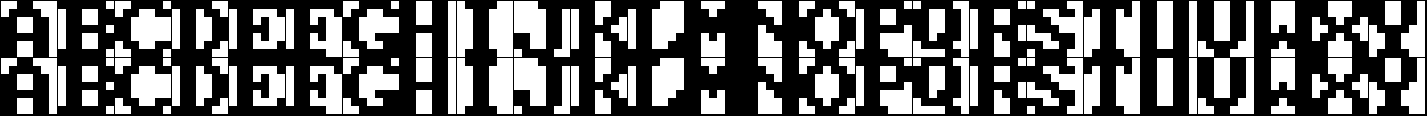
\includegraphics[width=12cm]{fig/im_both.png}
    \caption{Illustrating \textbf{the auto-associative training set} as 7x7 images, the first row being the input and the second the corresponding output of the patterns.}
\end{figure}

Lastly, I would like to clarify the following: While the reader may interpret 'perfect recall rate', and 'extraction rate' as two different measures, these are in fact considered to be the same, adapting the same conventions and notation as in the literature study, in chapter \ref{chpt:background}. The perfect recall rate, or extraction rate, denotes the number of extracted output patterns relative to the total number of output patterns in the training set, where extracted means a one to one correlation of the output patterns. Thus, perfectly recalled becomes equivalent to extracted, as a correlation of <1.0 is defined as a spuriously recalled pattern. As we will see, patterns tend to in fact be a lot more spurious, or be perfectly recalled, due to the hippocampal model's pattern completion qualities.
Furthermore, the spurious recall rate is always included either in the same graph, or in the next figure within the section, such that the reader may easily compare the perfect extraction rate with the spurious recall rate, as well as the convergence rate. This will hopefully make it easy to infer the quality of the extraction relative to some criteria, while making the original measures readily available. For instance, the perfect recall rate relative to the sum of all recalled patterns may be $1.0$, although the extraction rate is only $50 \%$, such as for some of the attained model schemes.

% ========================== EXPERIMENTS ============================          
\section{Hippocampal module experiments}\label{section:hpc-experiments}

Before I introduce the experiments, I would like to briefly introduce the hippocampal model functionality, by demonstrating model activity in a single experiment at a more detailed level. The intention of this is to create a more complete and sound picture of the model elements, as well as to provide the reader with a more thorough understanding of the representations that are used as input and output data. 
This is followed by experiments designed to test specific aspects of the hippocampal model, presenting aggregate results such as graphs of mean convergence ratios along with corresponding analyses.

% ============== subsection ================
\subsection{Low-level demonstration}

Following is a demonstration of hippocampal model learning, using two distinct model schemes for two different examples, with figures of model output after each learning iteration for chaotic recall and normal recall, i.e. pattern association. The first two subsets of auto-associative patterns, that is \{A$\rightarrow$A, B$\rightarrow$B\}, and \{C$\rightarrow$C, D$\rightarrow$D\}, are used as training sets in this example.
Furthermore, the hippocampal module is instantiated with the parametrization described above in tables \ref{table:initial_settings} and \ref{table:firing_rates}, and with a neuronal turnover rate $\tau = 0.04$ and a DG-weighting of $1$ in the first example, and $\tau=0.50$ and DG-weighting$=25$ in the second example. Neuronal turnover is performed between every learnt training set - that is, only once after learning the \{A$\rightarrow$A, B$\rightarrow$B\} associations, before commencing learning of the next input-output pair. Here the convergence criteria is set to a static number of training iterations, equal to $15$.
In further experiments, results are generated and analysed for both a dynamic convergence criterion for learning and stability during recall, as well as for two configurations of $i$ training iterations as the learning and stable recall criterion. Furthermore, the weight matrices are instantiated according to their respective firing rates, with weights being randomly assigned according to Gaussian distributions using the parameters presented in table \ref{table:initial_weight_distributions}, for the number of neurons corresponding to the layers' firing rates, respectively (as outlined in table \ref{table:firing_rates}).

Instantiating the hippocampal model using the parametrization as outlined above, images are generated of the network output for pattern recall (i.e. association), and chaotic recall for every training iteration. These are generated for both examples, i.e. synchronous and asynchronous updating of the CA3-layer in the model.

\begin{figure}
    \centering
    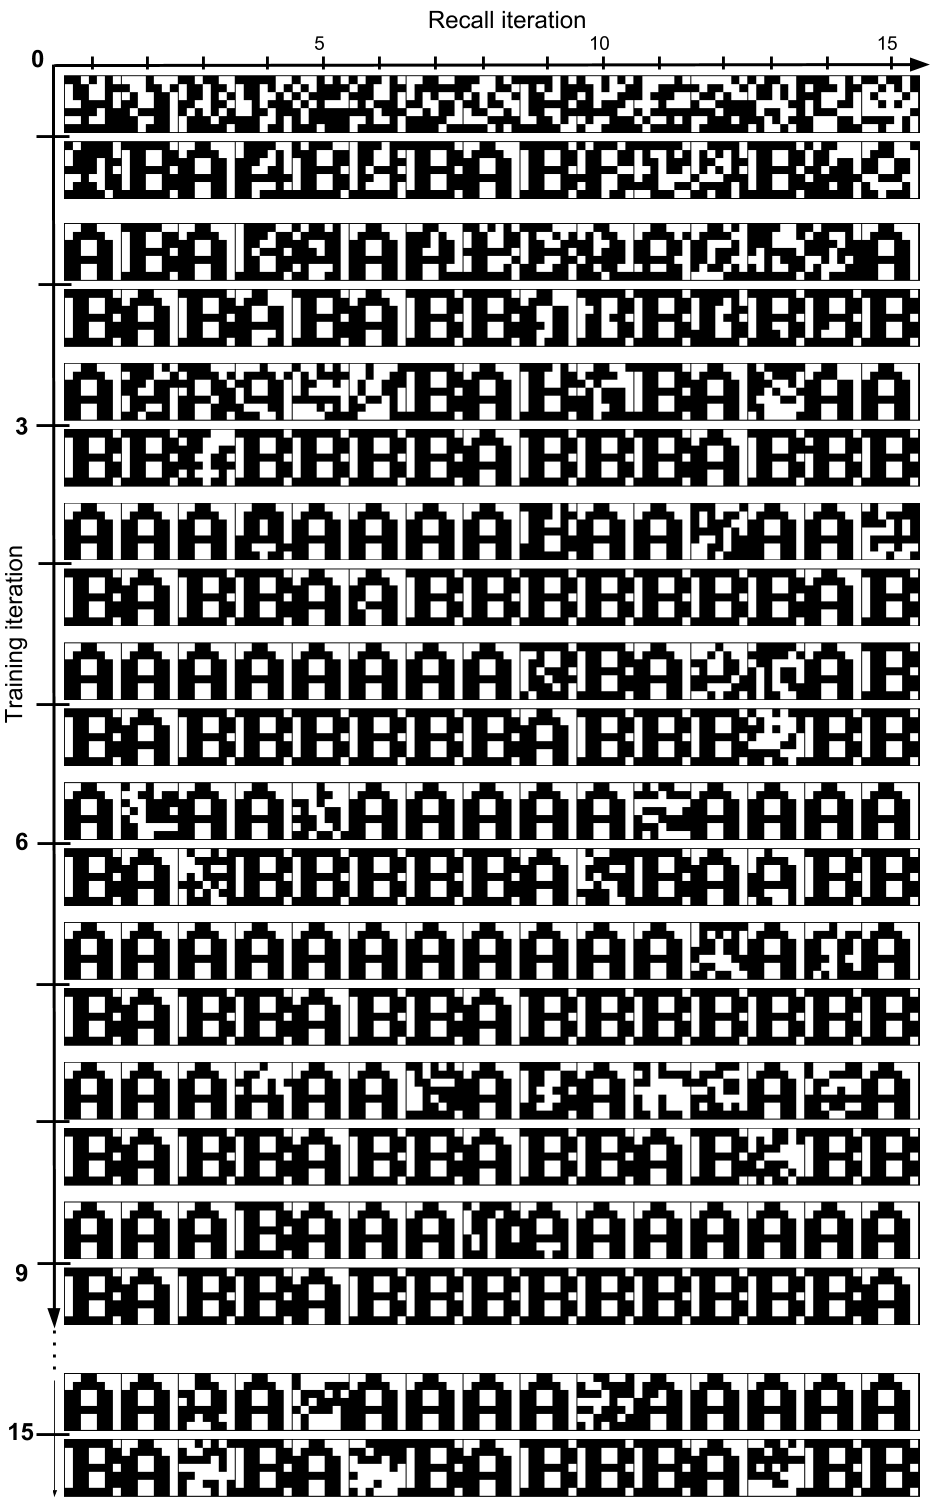
\includegraphics[width=10cm]{fig/AB-pattern-associations-sync-tm0-dgw25}
    \caption{Displaying the \textbf{neural network recall for the training inputs after each training iteration}. Note that the origin is now in the upper left corner, time flowing downward along the y-axis. Furthermore, the first axis denotes the model recall iterations. Note that for each training iteration, there are two rows of recalled output, displayed for two corresponding inputs, namely the two inputs of the current training subset. In this figure, these are the patterns 'A', and 'B', for the upper and lower rows, respectively. The model configuration is using synchronous CA3-updating, turnover only after the set is learnt, and a DG-weighting of 25.}
    \label{fig:pattern_associations_sync}
\end{figure}

\begin{figure}
    \centering
    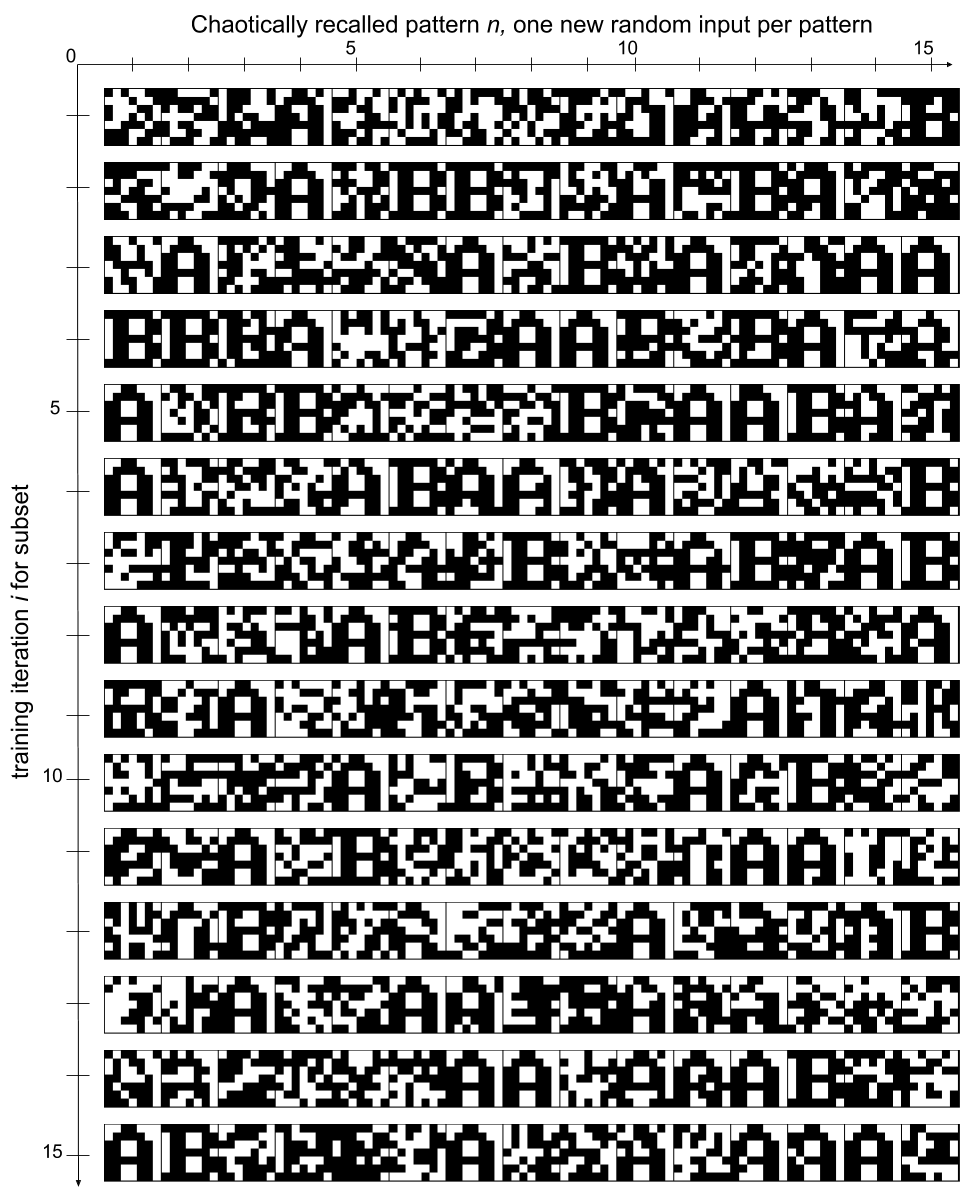
\includegraphics[width=11cm]{fig/AB-chaotic-recall-sync-tm0-dgw25}
    \caption{Displaying the \textbf{patterns recalled by chaotic recall} - that is, for each training iteration over the subset {A, B}, a random input is set as the input, for which the attained output after each recall iteration is displayed, for 15 iterations.}
    \label{fig:chaotic_recall_sync}
\end{figure}

When studying the two figures (\ref{fig:pattern_associations_sync}, \ref{fig:chaotic_recall_sync}) that display the recalled patterns during and after learning pattern-associations for patterns A$\rightarrow$A, and B$\rightarrow$B, note that pattern separation seems fairly successful, as the associated output for the aforementioned letters is fairly stable. However, some spurious patterns appear, even in the case of having the actual, non-distorted input of the pattern as the model's input. This may indicate weak model convergence, which may be due to incorrect model calibration, such as too heavy DG-weighting. Because the connections from the DG-layer are both instantiated as normally distributed with rather high weight values ($\mu=0.9, \sigma=0.01$), and weighted 25 times stronger than the connections from the EC- and CA3-layer, this may possibly disrupt the strength of the attained basins of attraction, or prolong the training period needed in order for the model to converge for its (EC-CA3, CA3-CA3, and thus CA3-output) connections, and thus for the CA3-layer to extract non-overlapping pattern-associations. The latter resulting in unstable behaviour within the auto-associative CA3-layer. 

Note that one run is not sufficient to determine whether this is the case. Therefore, these are parameters that will be tested in further experiments, where 20, or at least 10 trials per training set size, per configuration, are used in order to statistically determine patterns of the emergent model behaviour. I.e. At least 40-80 experiments per model configuration.

Lastly, it is worth noting that although model convergence and recall is fairly good in the case of having a non-distorted training pattern input as the network's input, a great number of spurious patterns are recalled in the chaotic recall scheme. Thus, the number spurious patterns extracted from chaotic recall is one of the measures that will be used in further analyses. Particularly with regards to successful pattern separation and the establishing of basins of attraction. I.e. the perfect recall rate may be erroneously observed as close to 100 \% of the number of training patterns - however, when the number of spurious patterns extracted by chaotic recall exceeds this number (possibly by a great deal), the quality of the model performance may still be considered poor. Note, however, that it might be interesting to also consider memory consolidation in such a scheme to the neocortical module. It might be that a functional mapping is contained within the recalled spurious patterns, as random inputs and outputs may still reflect parts of the functional mapping. 
Note that in the case of attaining a spurious pattern output for an input from the \textit{training set}, the functional mapping is most likely not present, and will only disrupt the convergence in the network which attempts to learn the pattern-associations. 
When it comes to the measures of model performance, another measure which will be used in terms of pattern consolidation is the goodness of fit measure, defined in the previous chapter (\ref{chpt:methods}).

% Furthermore, this instability, or oscillation between the model's basins of attraction, is further demonstrated in the figure of chaotically recalled patterns, which barely recalls the letters A and B, and mostly only spurious patterns that do not resemble the original input nor output patterns. Pattern separation is one of the aspects that are evaluated in this thesis. It is evaluated through successful convergence in the first configurations where the convergence criteria is defined as the output being stable for three iterations of recall. Furthermore, it is analysed in terms of all the configurations by considering the perfect recall rates, as well as spurious pattern recall rates.

In order to demonstrate another hippocampal model configuration, low level results are presented for the case of asynchronous updating of the CA3-layer in figures \ref{fig:pattern_associations_async} and \ref{fig:chaotic_recall_async}. Neuronal turnover is still only performed between the two learning sets, which may be argued to be biologically unrealistic (some recoding of weights, i.e. topological synaptic modification) may be argued to be continuously present, at a low rate, however. The latter is something that will be addressed in later experiments. 
Nonetheless, this constructed low level example introduces randomness in its training and recall by asynchronously updating the neurons of its CA3-layer for each training and recall iteration. This may be considered to be somewhat more biologically realistic, although still implausible in terms of only one neuron is updated at a time algorithmically in the implemented model. In a more biologically realistic model, all neurons should be updated simultaneously, where hard-ware level parallelism could potentially determine a pseudo-random order of neuronal updates, making sub-sets of neurons fire and wire simultaneously. 
However, as aggregate activity on the population level is what is studied in this thesis, I consider the attained results to yield valid results and associated suggestions at the neural network level.

\begin{figure}
    \centering
    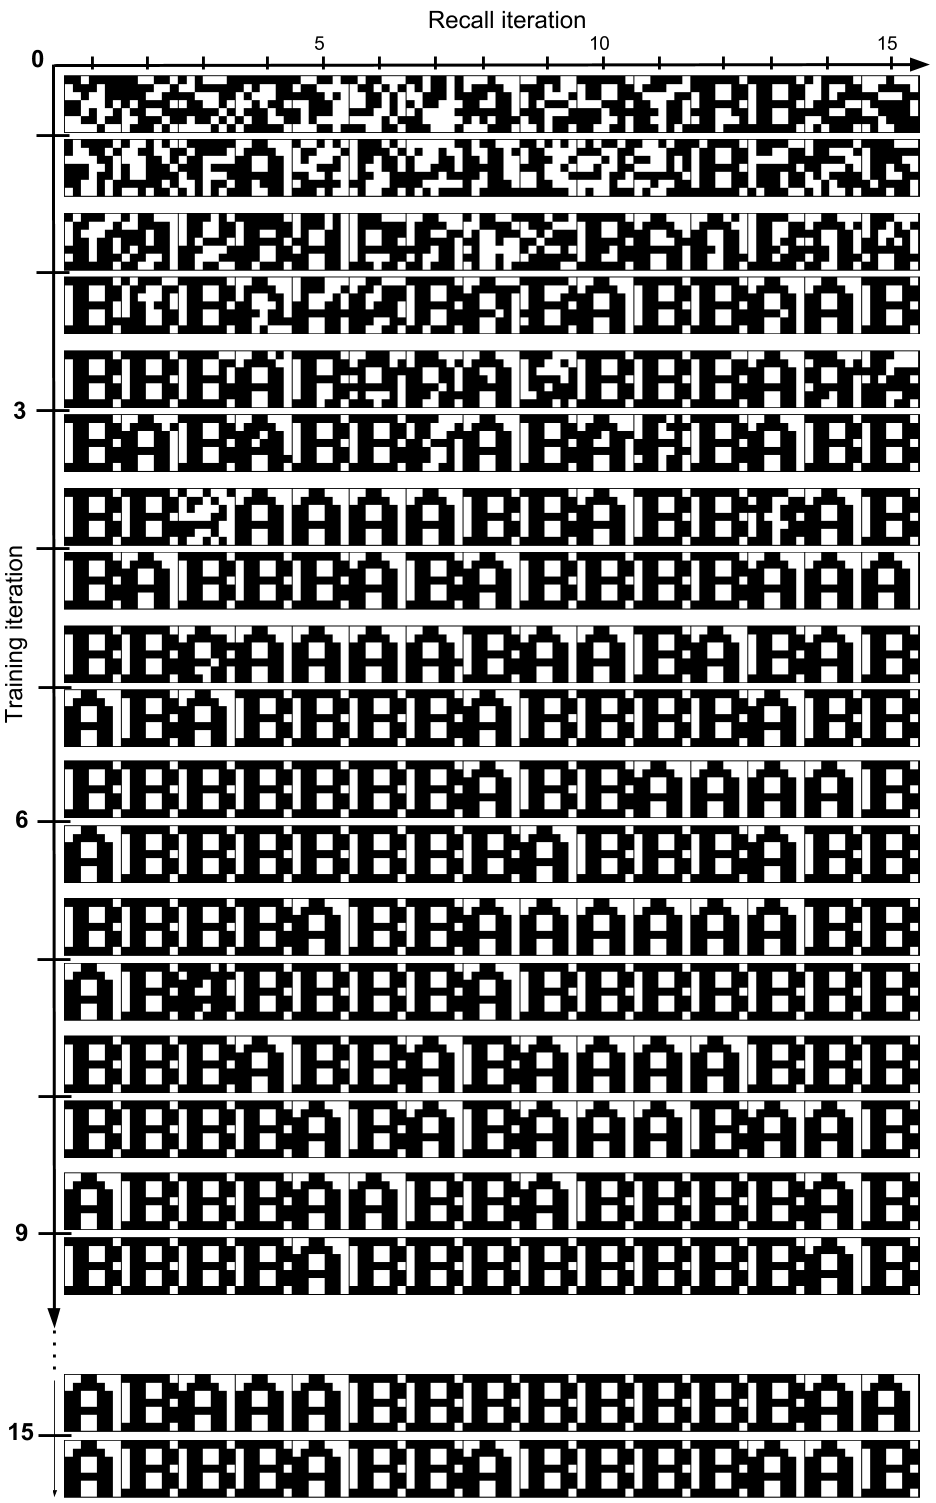
\includegraphics[width=10cm]{fig/AB-pattern-associations-async-tm0-dgw1-tau050}
    \caption{Showing the \textbf{recalled outputs for the training inputs of the subset}, after each subset training iteration, similar to in figure \ref{fig:pattern_associations_sync}. However, the model configuration used here is asynchronous CA3 udpating, neuronal turnover between every learnt set, a DG-weighting of 1, and $\tau=0.50$.}
    \label{fig:pattern_associations_async}
\end{figure}

\begin{figure}
    \centering
    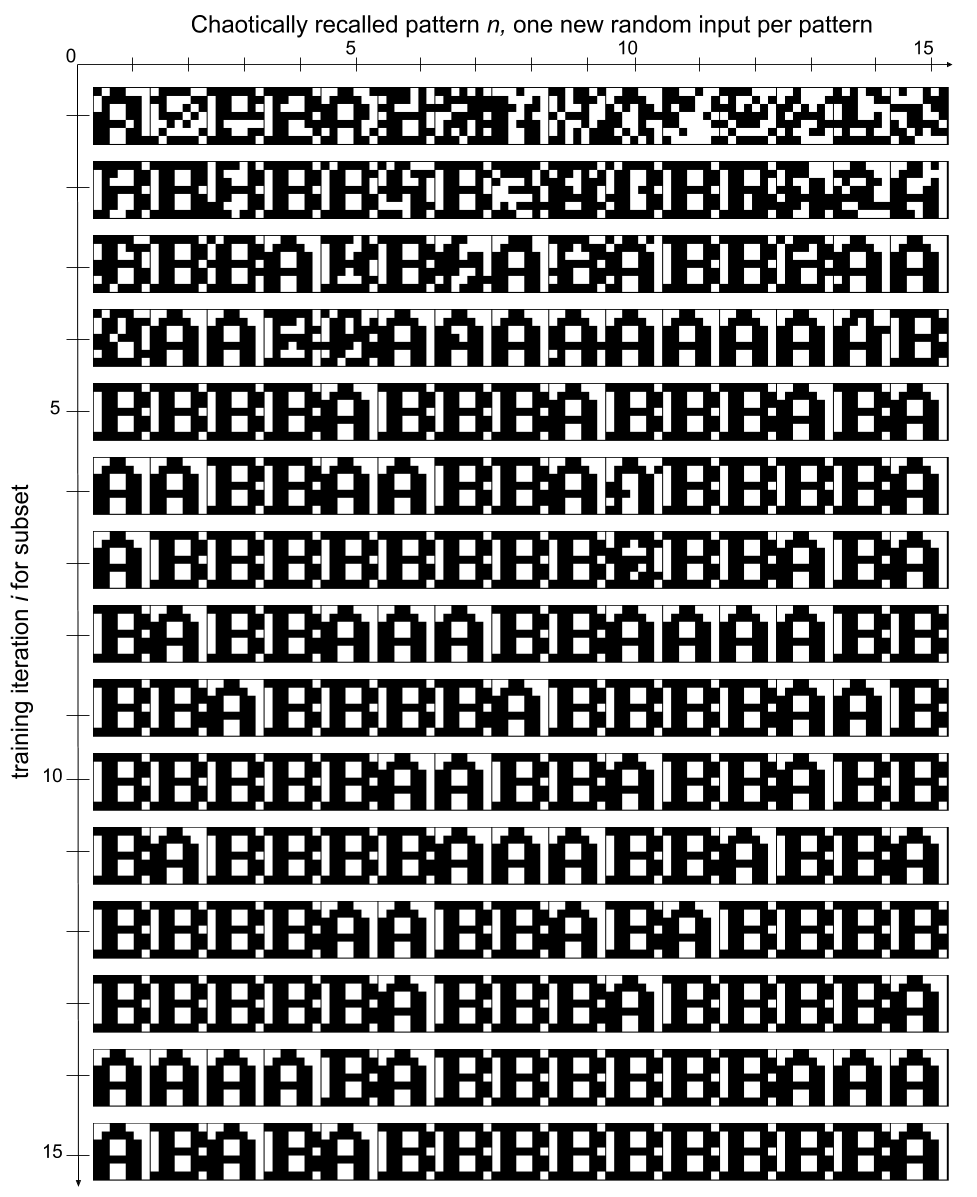
\includegraphics[width=11cm]{fig/AB-chaotic-recall-async-tm0-dgw1-tau050}
    \caption{Displaying the \textbf{chaotically recalled patterns} for the same model configuration and results as displayed in figure \ref{fig:pattern_associations_async} (asynchronous CA3-updating, a DG-weighting of 1, $\tau=0.50$, turnover between learnt sets). Note that spurious patterns diminishes very quickly, and only learnt patterns are chaotically recalled after very few iterations. This configuration seems to be capable of one-shot learning.}
    \label{fig:chaotic_recall_async}
\end{figure}

Note that while the quality of chaotic recall appears to be better in figures \ref{fig:pattern_associations_async}, and \ref{fig:chaotic_recall_async}, the scheme is less stable for the output for a learnt pattern association's input. This is expected, as more randomness is introduced in the random sequence of updating the neurons of the CA3-layer, which will tend to have the model find the other basin of attraction more easily. Because these results were attained from only one run, the generalizability is very constrained. Nevertheless, the results do suggest a trend towards a more specific extraction capability at the cost of less stability. It is worth keeping this in mind when considering further experiments and results. If the reader wishes to see the figures presenting the attained output for the next training set, i.e. subset of the training patterns, please refer to appendix D, in which they are contained.

% ============== subsection ================
% \subsection{Experiment 1: Schemes for updating the CA3-layer and performing neuronal turnover}
\subsection{Experiment: CA3-updating and neuronal turnover schemes}

In order to evaluate the impact of synchronous action potential propagation and synaptic weight modification, four different model schemes are used. These consist of combining two types of CA3-layer neuronal activation and weight modification with two types of neuronal turnover. More specifically; updating the CA3 neuronal activation values synchronously or asynchronously, and performing neuronal turnover between every learned training subset, or for every training iteration. Synchronous CA3-layer updating effectively results in reducing the propagation of values from one layer of neurons to another to a set of vector and matrix operations, whereas the asynchronous scheme requires updating each neuron independently. In the simplest case of synchronous updating, i.e. for all non-chaotic layers, the synchronous propagation scheme is simply reduced to a vector of activation values multiplied by a weight matrix, which is adjusted through the activation function. For each of these schemes; synchronous or asynchronous updating, two turnover modes are tested. Firstly, turnover is performed only once before every new training subset, i.e. between learnt training sets. Secondly, turnover is performed between every training set iteration - that is, for every iteration over the current subset.

In this experiment, 20 trials are performed for every full auto-associative training set (that is 2x5, 3x5, 4x5, and 5x5), for every configuration. In other words, for 20 trials $20 * 4 = 80$ experiments are run for each model configuration. In these experiments the model attempts to learn to associate the $n$ first capital letters auto-associatively, where $n$ corresponds to e.g. 2x5 $= 10$, 3x5$=15$, 4x5$=20$, or 5x5$=25$, the x denoting that the training set consists of 5 subsets that are used to train the model, sequentially. 
Furthermore, the convergence criterion is defined as the following: For each training pattern in the current training set, if the model output is the correct pattern output for the undistorted pattern-input for three recall iterations, the pattern is considered to be successfully learnt. If this is the case for every pattern in the current training subset, convergence is considered to be attained, and chaotic recall is performed. Furthermore, when generating figures, the model is considered to have successfully learned the current training set if converging in less than 50 training iterations. Chaotic recall is performed similarly to the procedure in \citep{Hattori2010, Hattori2014}. That is, during chaotic recall, when the output remains unchanged for three recall iterations, the pattern is considered to be learnt, or successfully extracted in the case of chaotic recall. Chaotic recall is always performed for 300 time-steps, with the input to the network being a new non-changing random input for every extracted pattern.


\begin{figure}
    \centering
    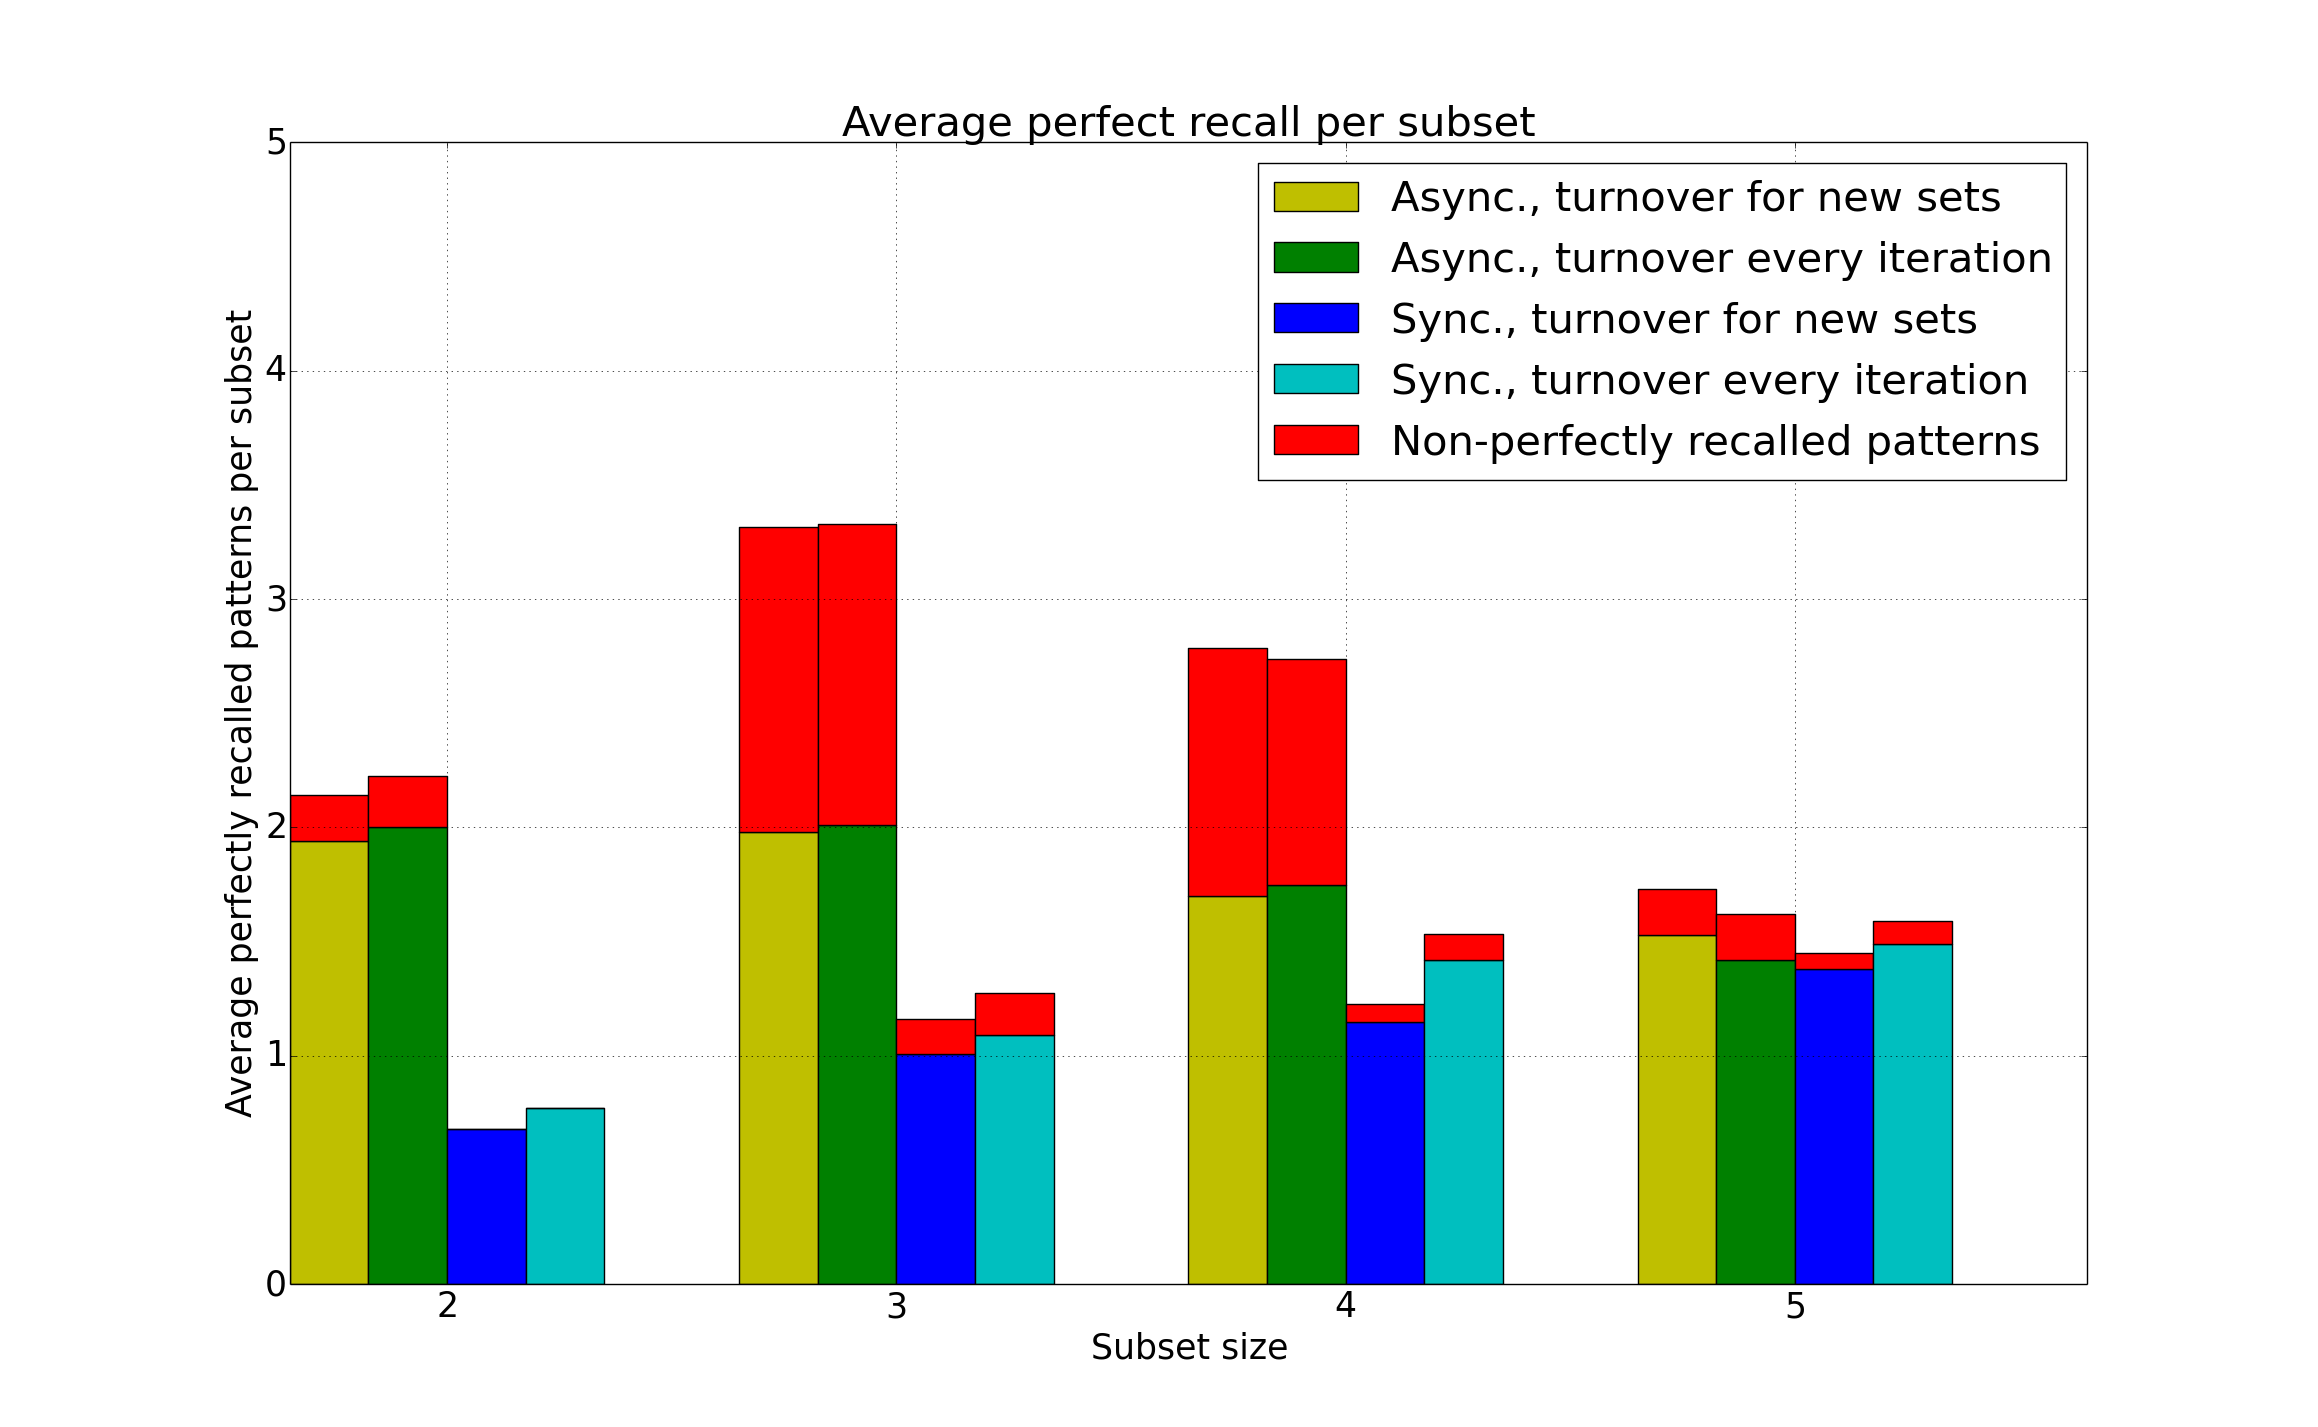
\includegraphics[width=14cm]{fig/average_perfect_recall_rates_by_set_size_with_spurious_bars}
    \caption{Displaying the average number of perfectly recalled patterns for each model configuration, along with the average number of spuriously recalled patterns for each configuration. Note that the dentate gyrus weighting is set to 25, and the turnover rate to $0.50$ in all of the configurations, which might impact particularly the turnover mode in which turnover is performed between every training iteration.}
    \label{fig:avg_perfect_recall_rates_with_spurious_bars}
\end{figure}

Note that spurious is defined as any distinct non-perfectly recalled pattern in figure \ref{fig:avg_perfect_recall_rates_with_spurious_bars}. Non-perfect is used as a term rather than imperfect to signify that the pattern may be either nearly perfect, or in fact completely random, i.e. spurious. Note that in contrast to the introductory examples where the convergence criterion was defined as training or recalling for a fixed number of iterations \textit{i}, (\textit{i} $=15$ in the introductory low-level examples), having a stricter convergence criterion naturally resulted in no spurious patterns being recalled in the synchronous updating schemes, which may be expected when considering figure \ref{fig:chaotic_recall_sync}. However, it remains unclear whether model convergence is attained successful in terms of pattern separation. In order to possibly elucidate this, the convergence rate is also considered, and presented in figure \ref{fig:convergence_rates_async_sync} for asynchronous CA3 updating.

\begin{figure}
    \centering
    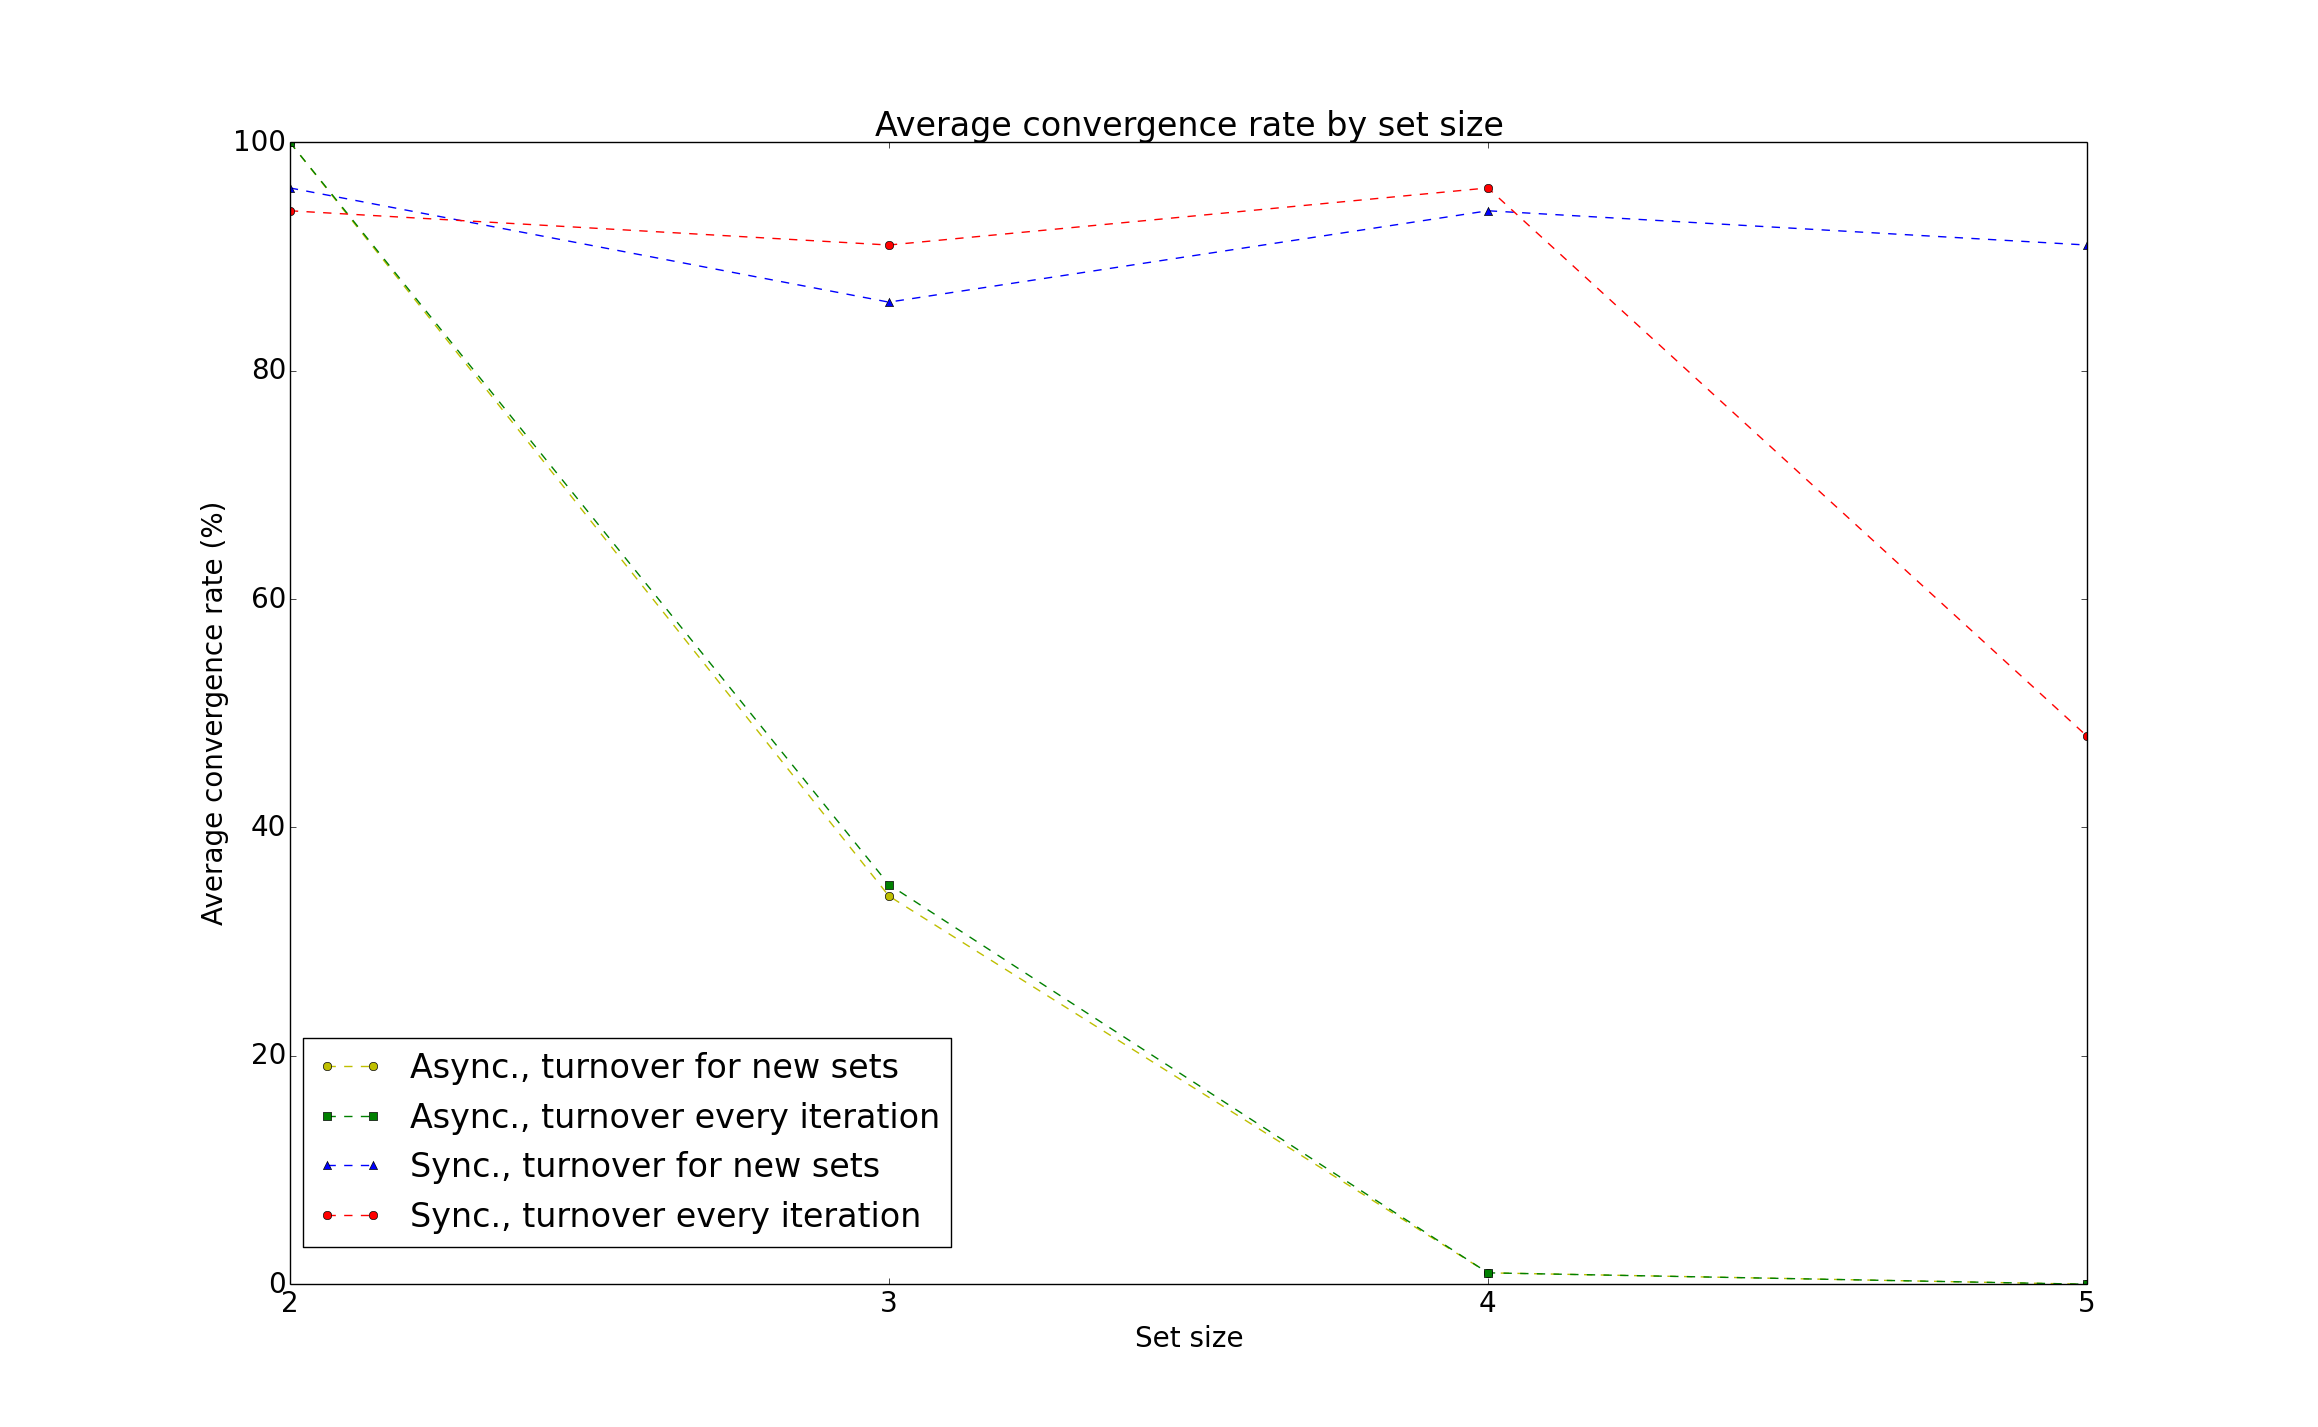
\includegraphics[width=14cm]{fig/avg_convergence_rate}
    \caption{Presenting the average convergence rate in the four experiment-schemes, using the strict convergence criterion. Learning and convergence is considered successful if attained within 50 training iterations. Note that the synchronous updating schemes seem to converge significantly better than the asynchronous. Furthermore, when employing neuronal turnover for every training iteration, the convergence rate does not seem to fall as the set size increases.}
    \label{fig:convergence_rates_async_sync}
\end{figure}

Although extraction of all patterns using chaotic recall is unsuccessful in nearly all of the current experiment schemes, one of the synchronous schemes, using turnover for every training iteration, converges well for all set sizes. However, it remains the scheme which performs the worst in terms of the perfect recall rate.
Furthermore, this scheme recalls nearly no other than 1-2 of the patterns from each training subset, which it recalls perfectly. 
This may suggest that while the scheme is likely to successfully be able to separate patterns during training, it might not be able to separate them well enough to be able to chaotically recall them. Or even more likely; it might be that the chaotic recall criterion, being the same as the convergence criterion during training, is too stringent. I.e. a stability criterion of having the same output for three training iterations may be sensible when the correct pattern input is given to the network. However, when a random input is provided, it is expected that the network will oscillate more, and thus be less stable in its basins of attraction. Therefore, a relaxed convergence criterion might be more sensible during recall.

% Some hypotheses on why training is successful in nearly all cases, but not extraction by chaotic recall, include the following:
% - It may simply be that the model adjusts its weights too heavily towards the present firing patterns. However, this hypothesis remains implausible as the convergence criterion ensures that the model is fairly stable for every pattern in the training subset, i.e. the output remains correct for three recall iterations when the corresponding input of the pattern is presented to the network. This is the case in nearly 100 \% of the training cases, unaffected by set size.
Because every neuron of the CA3-layer is updated synchronously, it may also be that the model lacks a certain 'jiggle' during recall, making it prone to being stuck in a subset of its basins of attraction. This view is further strengthened by considering that the DG-layer is not used during recall, as it performs expansion encoding, which along with its sparsity may recode and separate similar, but distinct, inputs into separate patterns for the CA3-layer to then be able to auto-associatively learn. Because convergence is attained during training, but not recall, this suggests that the DG-layer may in fact give rise to these emergent qualities, but that the CA3-layer possibly favours a subset of the learnt patterns too strongly, resulting in pattern completion for only this subset of patterns.
% - Another view, which of course may very possibly be intertwined with the former is that

Note that due to the quick learning capability of the hippocampal module, it is unlikely that the EC to CA3 connections, as well as the CA3-CA3 connections have not been able to converge towards the solutions and extracted pattern correlations. However, if the recoding does not settle into a steady pattern, changing the input to the CA3-layer significantly for every training iteration, it may of course be the case that the weights do not converge. This theoretical scenario, however, is very unlikely to occur, as k-WTA will strengthen the connection weights to the first k winners, thus tending to favor the initial winners for the same input, only changing the output which it projects to the CA3-layer very little, if at all. 
This is exactly the reason for why neuronal turnover is performed in the first case - to recode the weight configuration such that the resulting k winners will vary slightly more, thus furthering its recoding abilities, potentially improving pattern separation and model performance. Note that it is the expansion encoding and sparsity in the DG-layer that recodes and separate similar, but distinct patterns. Together with the input of the EC-layer, the current values of the CA3-layer results in updating of weights for the recurrent connection to the layer itself, as well as backwards through the DG- and EC-layer, which again are adjusted according to the 'observed' input for the current pattern. In other words, a desired model configuration is when the model dynamically separates patterns due to its recoding qualities, and yet is able to recall them without the use of the pathways which expand, recode and project its values which separates the patterns.
% refactor:
It may be argued that completely omitting the DG-layer during recall is somewhat unrealistic. 
However, according to physiological findings, the DG-CA3 pathway is used very little during recall \citep{Wakagi2008}, justifying the omission during recall. 
Furthermore, due to the auto-associative nature of the CA3-layer, if this layer has successfully converged for patterns with little overlap, it is likely to fall into a basin of attraction, performing pattern completion for partial pattern input. Now, one may think that the EC-layer will not necessarily project a partial, recoded pattern to the CA3-layer, as this recoding is performed in synergy with the DG-layer. However, as the observant reader may have noticed, it is exactly that; in \textit{synergy} with the DG-layer, and as recoding has already been performed, this recoding is propagated to all layers of the network model by the Hebbian learning. In other words, the synaptic weight modification between the EC-layer and CA3 will reflect the recoded pattern. Furthermore, if only partially reflecting it, the CA3-layer may perform pattern completion.

Lastly, the nature of the CA3-neurons, i.e. chaotic neurons, may also impact the chaotic recall capabilities of the model. While it appears evident that the zeta- and eta-equations do not limit successful training of patterns, it may be that they impact the next activation values of the CA3-layer too heavily during recall. This may be argued by considering that in the current implementation, the next eta- and thus zeta-values are based on the former eta- and zeta-values along with the sum of the raw input sum, i.e. the sum of the dot products between the anteceding layers' activation value vectors and their corresponding weight matrices, without computing the values' transfer function values. 
However, as damping factors are used, the former values will be disregarded at an exponential pace. Leaving only the possibility that the sum of the former values along with the new input sum enhances the gravity of the current basin of attraction. This is unlikely, as the model attains successful convergence for an additional term in the input equation during training, namely the dot product from the DG-layer. Furthermore, this product may be multiplied by a factor up to 25. If anything, this may suggest that the eta- and zeta-functions are not at all excited about the DG-layer's absence, possibly resulting in its stable mood.


% ========================== DGWs ===============================
\subsection{Experiment: Dentate Gyrus Weighting}

In \citeauthor{Wakagi2008}'s \citeyear{Wakagi2008} hippocampal model, upon which \citeauthor{Hattori2010}'s \citeyear{Hattori2010, Hattori2014} models are based, the DG-layer, performing separation of similar, yet distinct patterns, has the ability to influence the activity of the CA3 strongly during learning. The idea that the DG is able to strongly influence the activity of CA3 during learning, is also confirmed by physiological findings \citep{Rolls1998chpt6}, and employed in work such as \citep{Norman2003}.

When it comes to this thesis' model; as synaptic connections from DG to CA3 are used solely during learning, this may in fact be what is needed in order to encompass and attain the desired emergence of successful pattern separation. Note also that the DG-CA3 weight matrix is initialized with rather high weight values ($\mu=0.9, \sigma=0.01$), and a low deviation from those values for the neurons whose synaptic connections become instantiated. This may result in the layer being able to highly influence preceding neurons through its connections. However, this does not necessarily hold, as weights from EC-CA3 may grow towards 1 as well. In either way, I decided to model the potential impact of adjusting the DG-weighting by implementing a DG-CA3 weight matrix \textit{coefficient}, also referred to as the DG-weighting. For each DG-weighting variable value from 0 to 29, 40 experiments are performed - i.e. 10 experiments per set size. Furthermore, these experiments are performed for four different hippocampal model configurations, namely:

%list
\begin{enumerate}  
\item Asynchronous updating of the CA3-layer values and weights, turnover for every training iteration, using a turnover rate $\tau=0.04$.
\item Asynchronous updating of the CA3-layer, with neuronal turnover between learnt training subsets, $\tau=0.50$.
\item Synchronous updating of the CA3-layer and its associated values and weights, turnover for every new training subset, $\tau=0.50$.
\item Synchronous updating of the CA3-layer and its associated values and weights, turnover for every training iteration, $\tau=0.04$.
\end{enumerate}

Note that the model configuration now employs a turnover rate, denoted by $\tau$, of $\tau=0.04$ in the neuronal turnover schemes where turnover is performed for every training iteration. This is due to the fact that performing turnover for  $50 \%$ of the neurons between learnt training subsets, does in fact result in less neurons being re-initialized than when performing turnover for every training iteration, when the number of iterations $i$ are above $12$ before reaching convergence. Furthermore, $\tau=0.04$ is, albeit performing turnover implausibly frequently, a more biologically realistic rate in itself. 
Nevertheless, employing the different rates does algorithmically test slightly different model parametrization and computation aspects. Even though turnover for every training set iteration may be unrealistic, the may provide a basis for further analysis on the topic of randomness in the DG-layer, as well as whether the model may be linked to some hippocampal functional aspects that operate at a larger time-scale.

% results

\begin{figure}
    \centering
    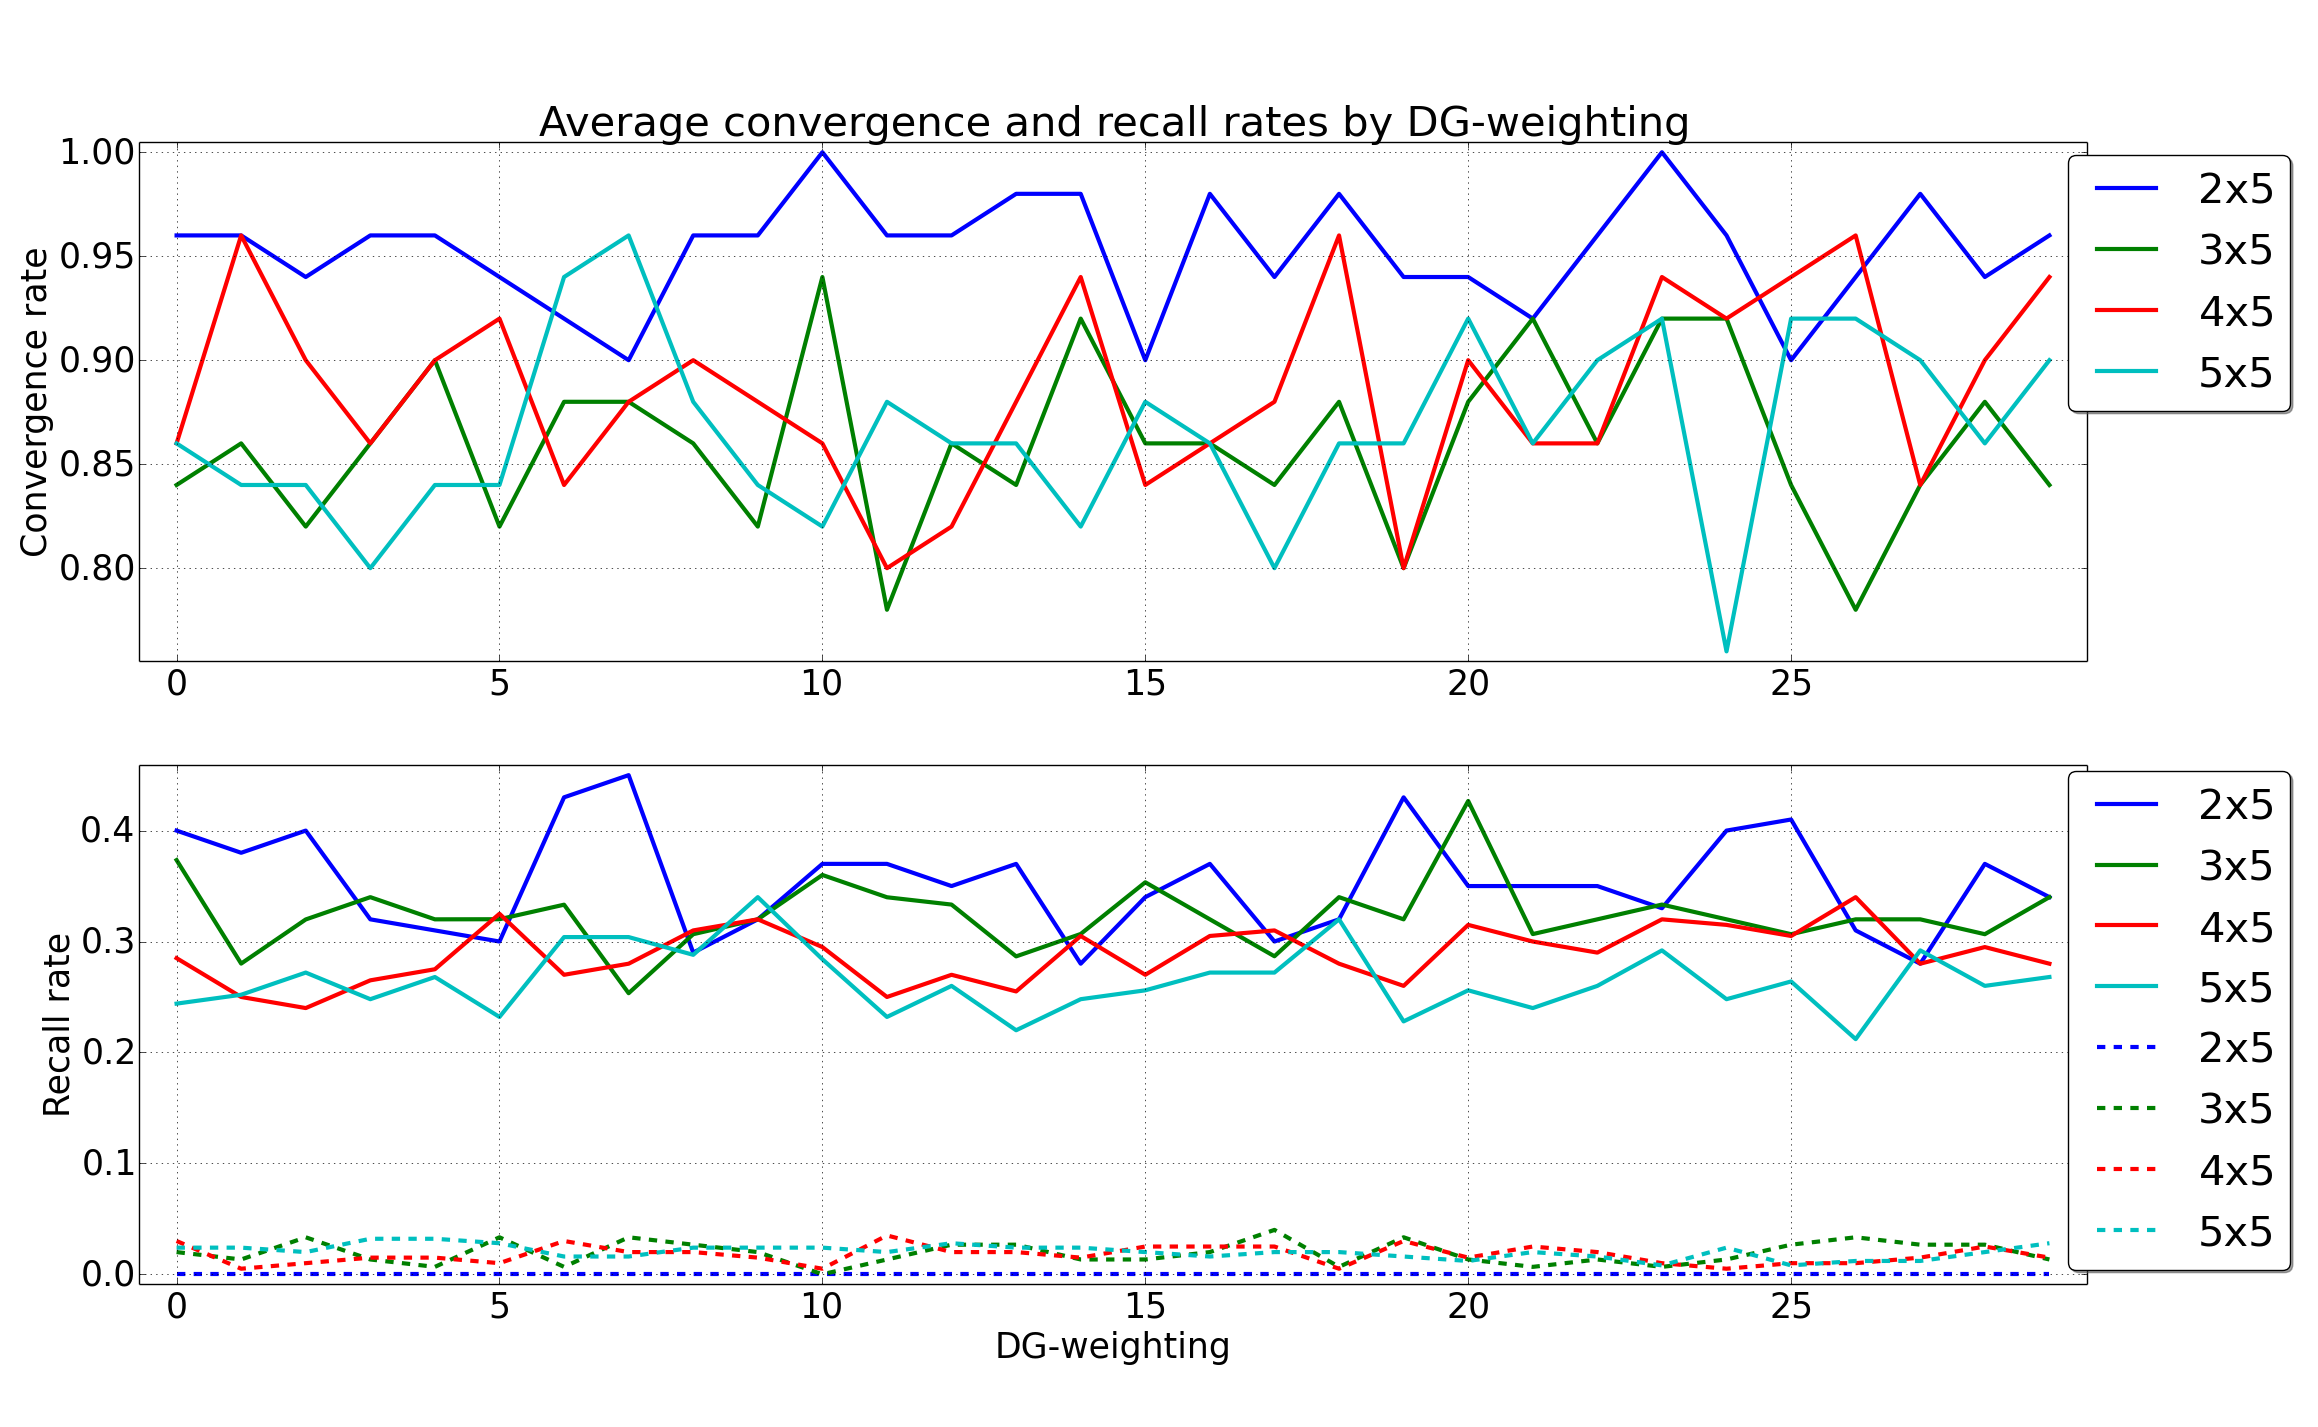
\includegraphics[width=13cm]{fig/DGWs/sync_tm0_50}
    \caption{Displaying the \textbf{convergence rate (upper subplot) and recall rates (lower subplot) by DG-weighting} for the scheme of synchronous CA3-layer neuronal updates, using a turnover rate $\tau=0.50$, and neuronal turnover between learnt subsets. Note that the dashed lines in the lower subplot denote the spurious recall rates, whereas the continuous lines indicate the perfect recall rates of the corresponding set sizes. It seems that using the DG-layer altogether does not impact the extraction rate of the model with the current parametrization. Furthermore, the extraction rate relative to the pattern size of perfectly recalled patterns remains fairly uniform across all training set sizes.}
    \label{fig:sync_tm0_50}
\end{figure}

\begin{figure}
    \centering
    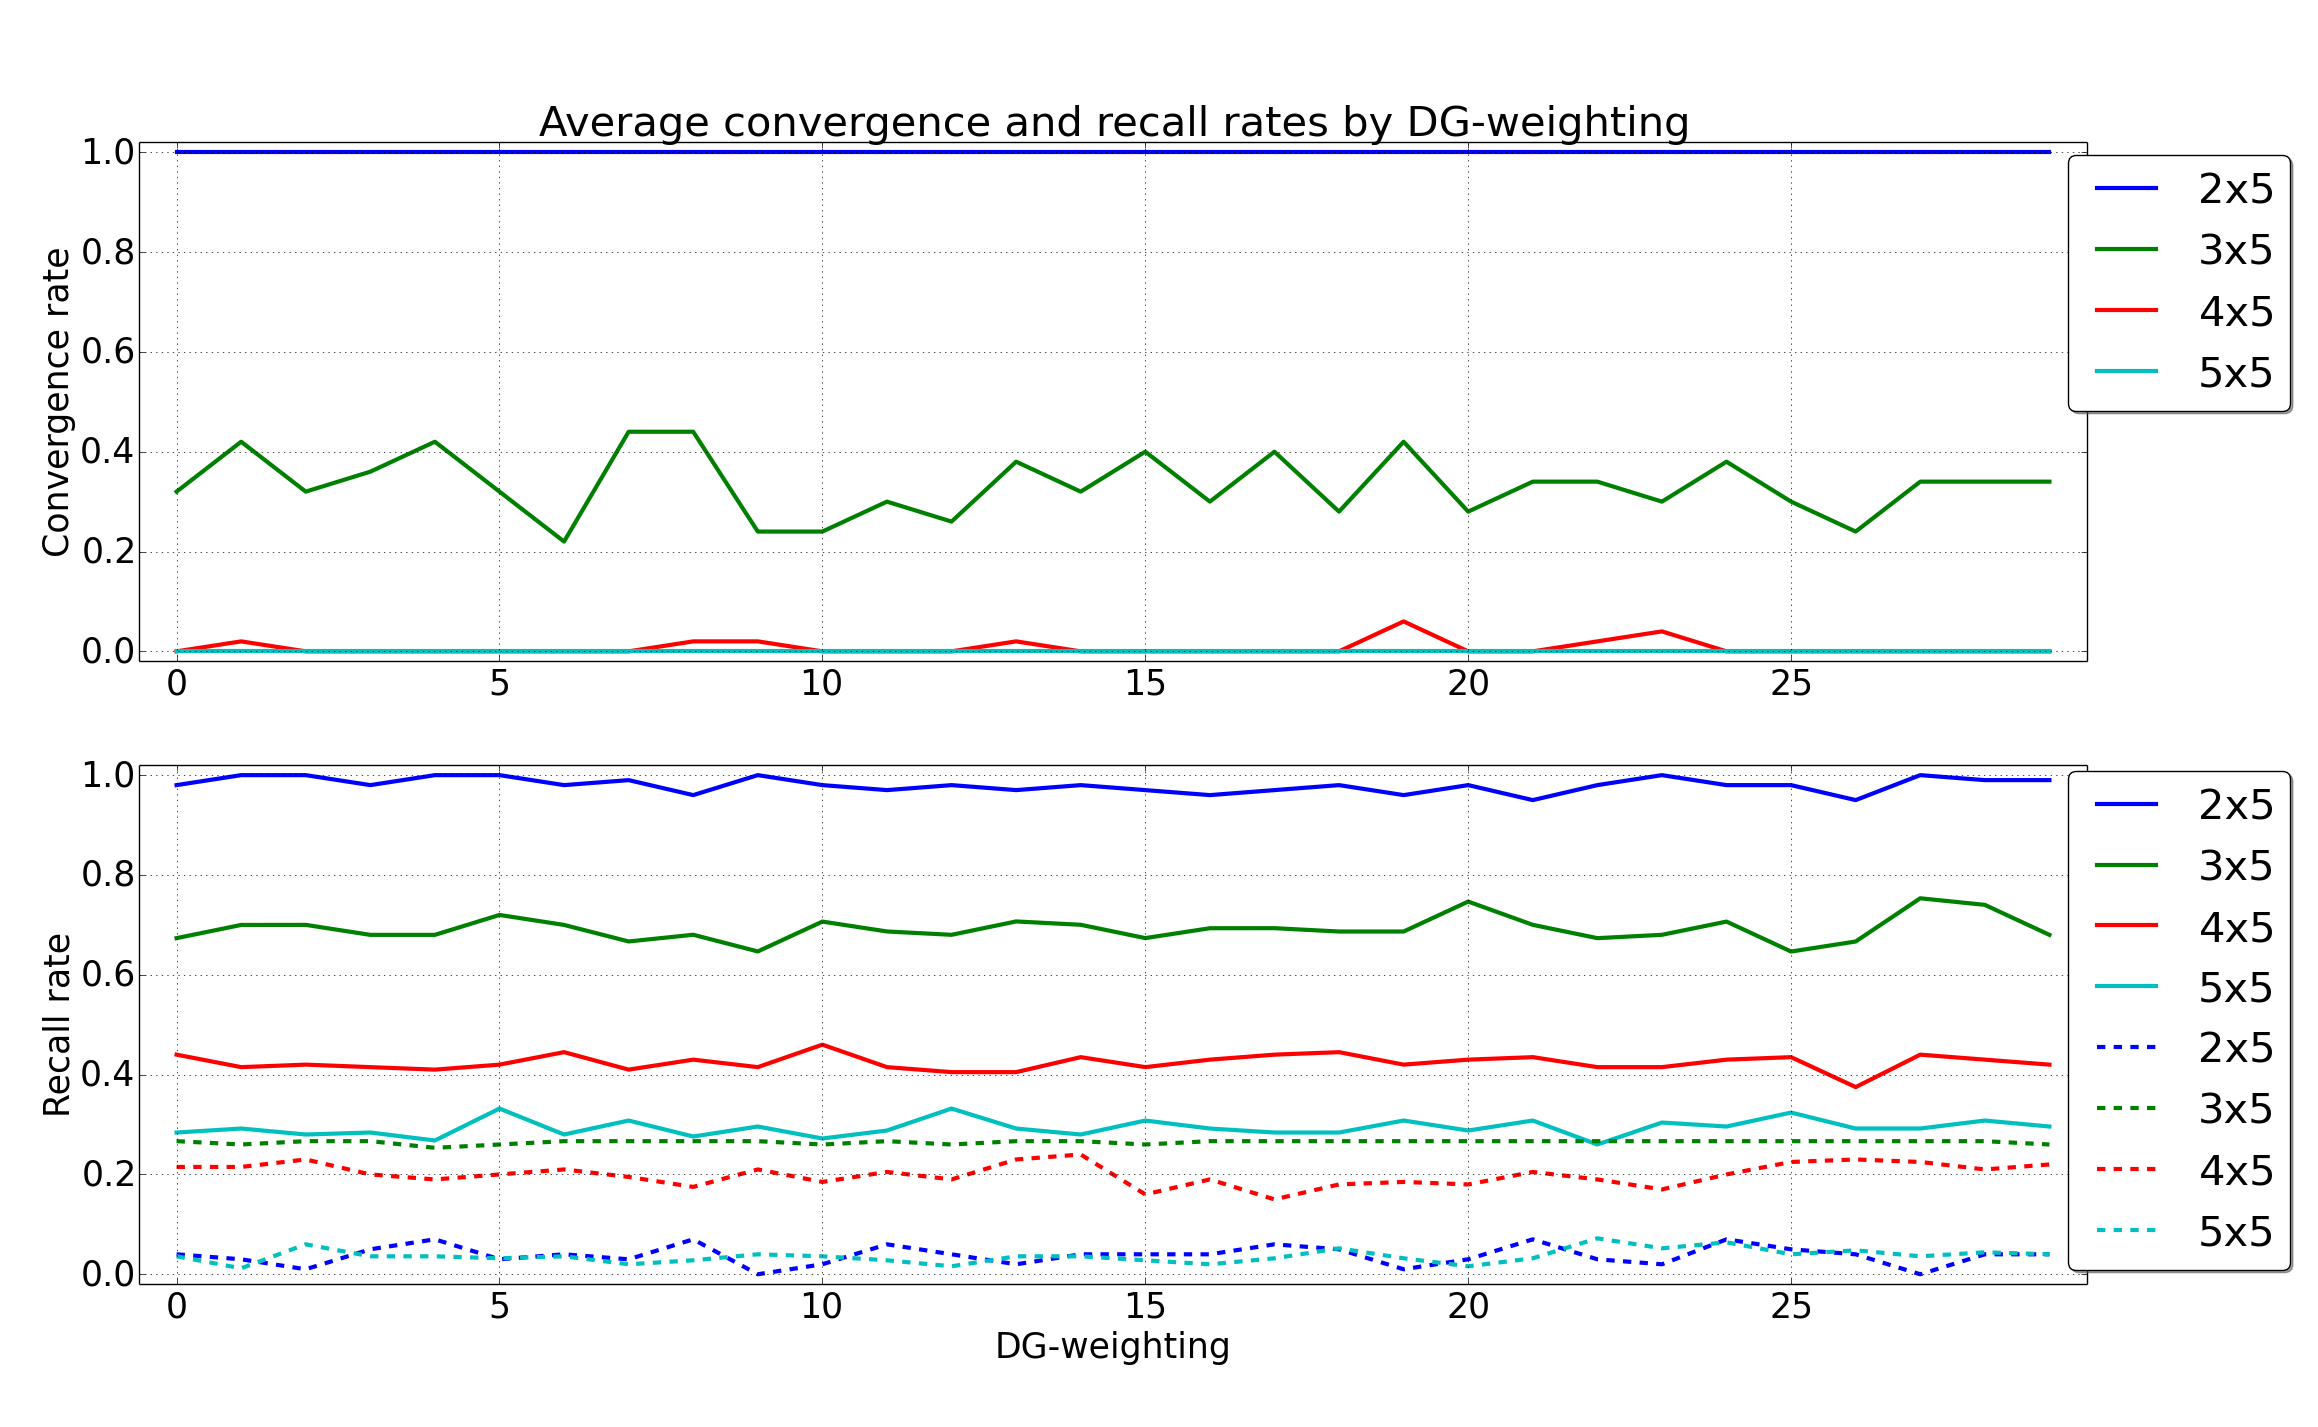
\includegraphics[width=13cm]{fig/DGWs/async_tm0_50}
    \caption{Displaying the \textbf{recall rates by DG-weighting} as in \ref{fig:sync_tm0_50}, however here for the configuration of asynchronous CA3 updating, and with $\tau=0.50$, turnover being performed between learnt sets. Interestingly, note that when convergence is near perfect \textit{and} very poor, no spurious patterns are extracted.}
    \label{fig:async_tm0_50}
\end{figure}

Note in figure \ref{fig:sync_tm0_50} that the perfect recall rate is fairly equal for all training set sizes. This may indicate that either few basins of attractions are formed, or that only few basins are reached during chaotic recall. As the model converges in nearly 100 \% of the cases, the latter is likely to be the case. Figures for synchronous CA3-layer updating, using turnover for every set iteration, with the neuronal turnover rate $\tau=0.04$, are included in appendix D. These figures are very similar to the ones attained for the scheme using turnover for every new set only, with $\tau=0.50$.

As for the DG-weighting itself, note that there seems to be no significant correlation nor performance gain with the DG-weighting. Therefore, pattern separation from the DG-CA3-connections seem to be largely unsuccessful during recall.
Note also that discarding the activity of the layer altogether during learning does not result in significantly worse model performance, which strengthens the hypothesis that the activity of the DG-layer is unsuccessful in heavily influencing the activity of the CA3-layer. 
This may be the case due to the synchronicity in the CA3-updates. 
However, when looking at the figures for the asynchronous CA3 updating schemes, both schemes generate very similar figures. Note that the turnover mode with turnover between learnt subsets only is also the only included figure for the synchronous model scheme in this chapter, the latter being contained within appendix D.
Furthermore, the poor convergence results in approximately no spuriously recalled patterns. This could suggest that the two other set sizes partly successfully separate patterns. However, when considering that the convergence rate drops rapidly when increasing the training set size, this suggests that pattern separation is unsuccessful, as introducing more patterns (and more overlap) results in very poor model performance. Furthermore, the recall rates for both perfect recall and spurious recall are highly correlated with the convergence rate, which strongly suggests that introducing asynchronicity may increase the perfect recall rate, but does so highly due to the increase in randomness, including spuriously recalled patterns. Furthermore, the model performance for the largest set size is so poor that it may only learn to recall one to two patterns for set sizes 4x5 and 5x5. These basins of attraction are the only ones that the model may converge towards, also strengthening the claim that the model capacity is reduced to one or two patterns due to unsuccessful pattern separation.


% ======================= turnover rates ========================
\subsection{Experiment: Neuronal turnover rates}

As the neuronal turnover rate may directly impact the model's separation capabilities, and is shown to be correlated with model performance by \citep{Hattori2014}, I here investigate model convergence, perfect recall rate and spurious pattern recall rate, here defined as non-perfect pattern recall, relative to the turnover rate for several model schemes, see table \ref{table:turnover_schemes}. These experiments may elucidate why pattern separation was unsuccessful for all of the DG-weightings in the former experiments.

\begin{table}[]
\centering
\caption{Showing the setup schemes used for investigating the impact of the neuronal turnover rate on model performance. Note that neuronal turnover modes 0, and 1, correspond to turnover between every learnt set, and turnover for every training iteration, respectively.}
\label{table:turnover_schemes}
\begin{tabular}{|c|c|c|}
\hline
\multicolumn{3}{|c|}{Setup}                               \\ \hline
CA3 updating mode & DG-weighting & Turnover mode        \\ \hline
Async             & 1            & 0                      \\ \hline
Async             & 25           & 0                      \\ \hline
Async             & 1            & 1                      \\ \hline
Sync              & 1            & 0                      \\ \hline
Sync              & 25           & 0                      \\ \hline
Sync              & 25           & 1                      \\ \hline
\end{tabular}
\end{table}

Interestingly, the asynchronous updating mode and dentate granule neurons' weighting seemed to to have no impact on model performance, nor did varying the turnover rate, $\tau$. Note that asynchrounous CA3-updating, along with a DG-weighting of 25 and turnover mode 1 is not tested. This is justified by considering that the DG-weighting had no impact on model behaviour in the previous experiments under this configuration (figure \ref{fig:async_tm1_04}).

\begin{figure}
    \centering
    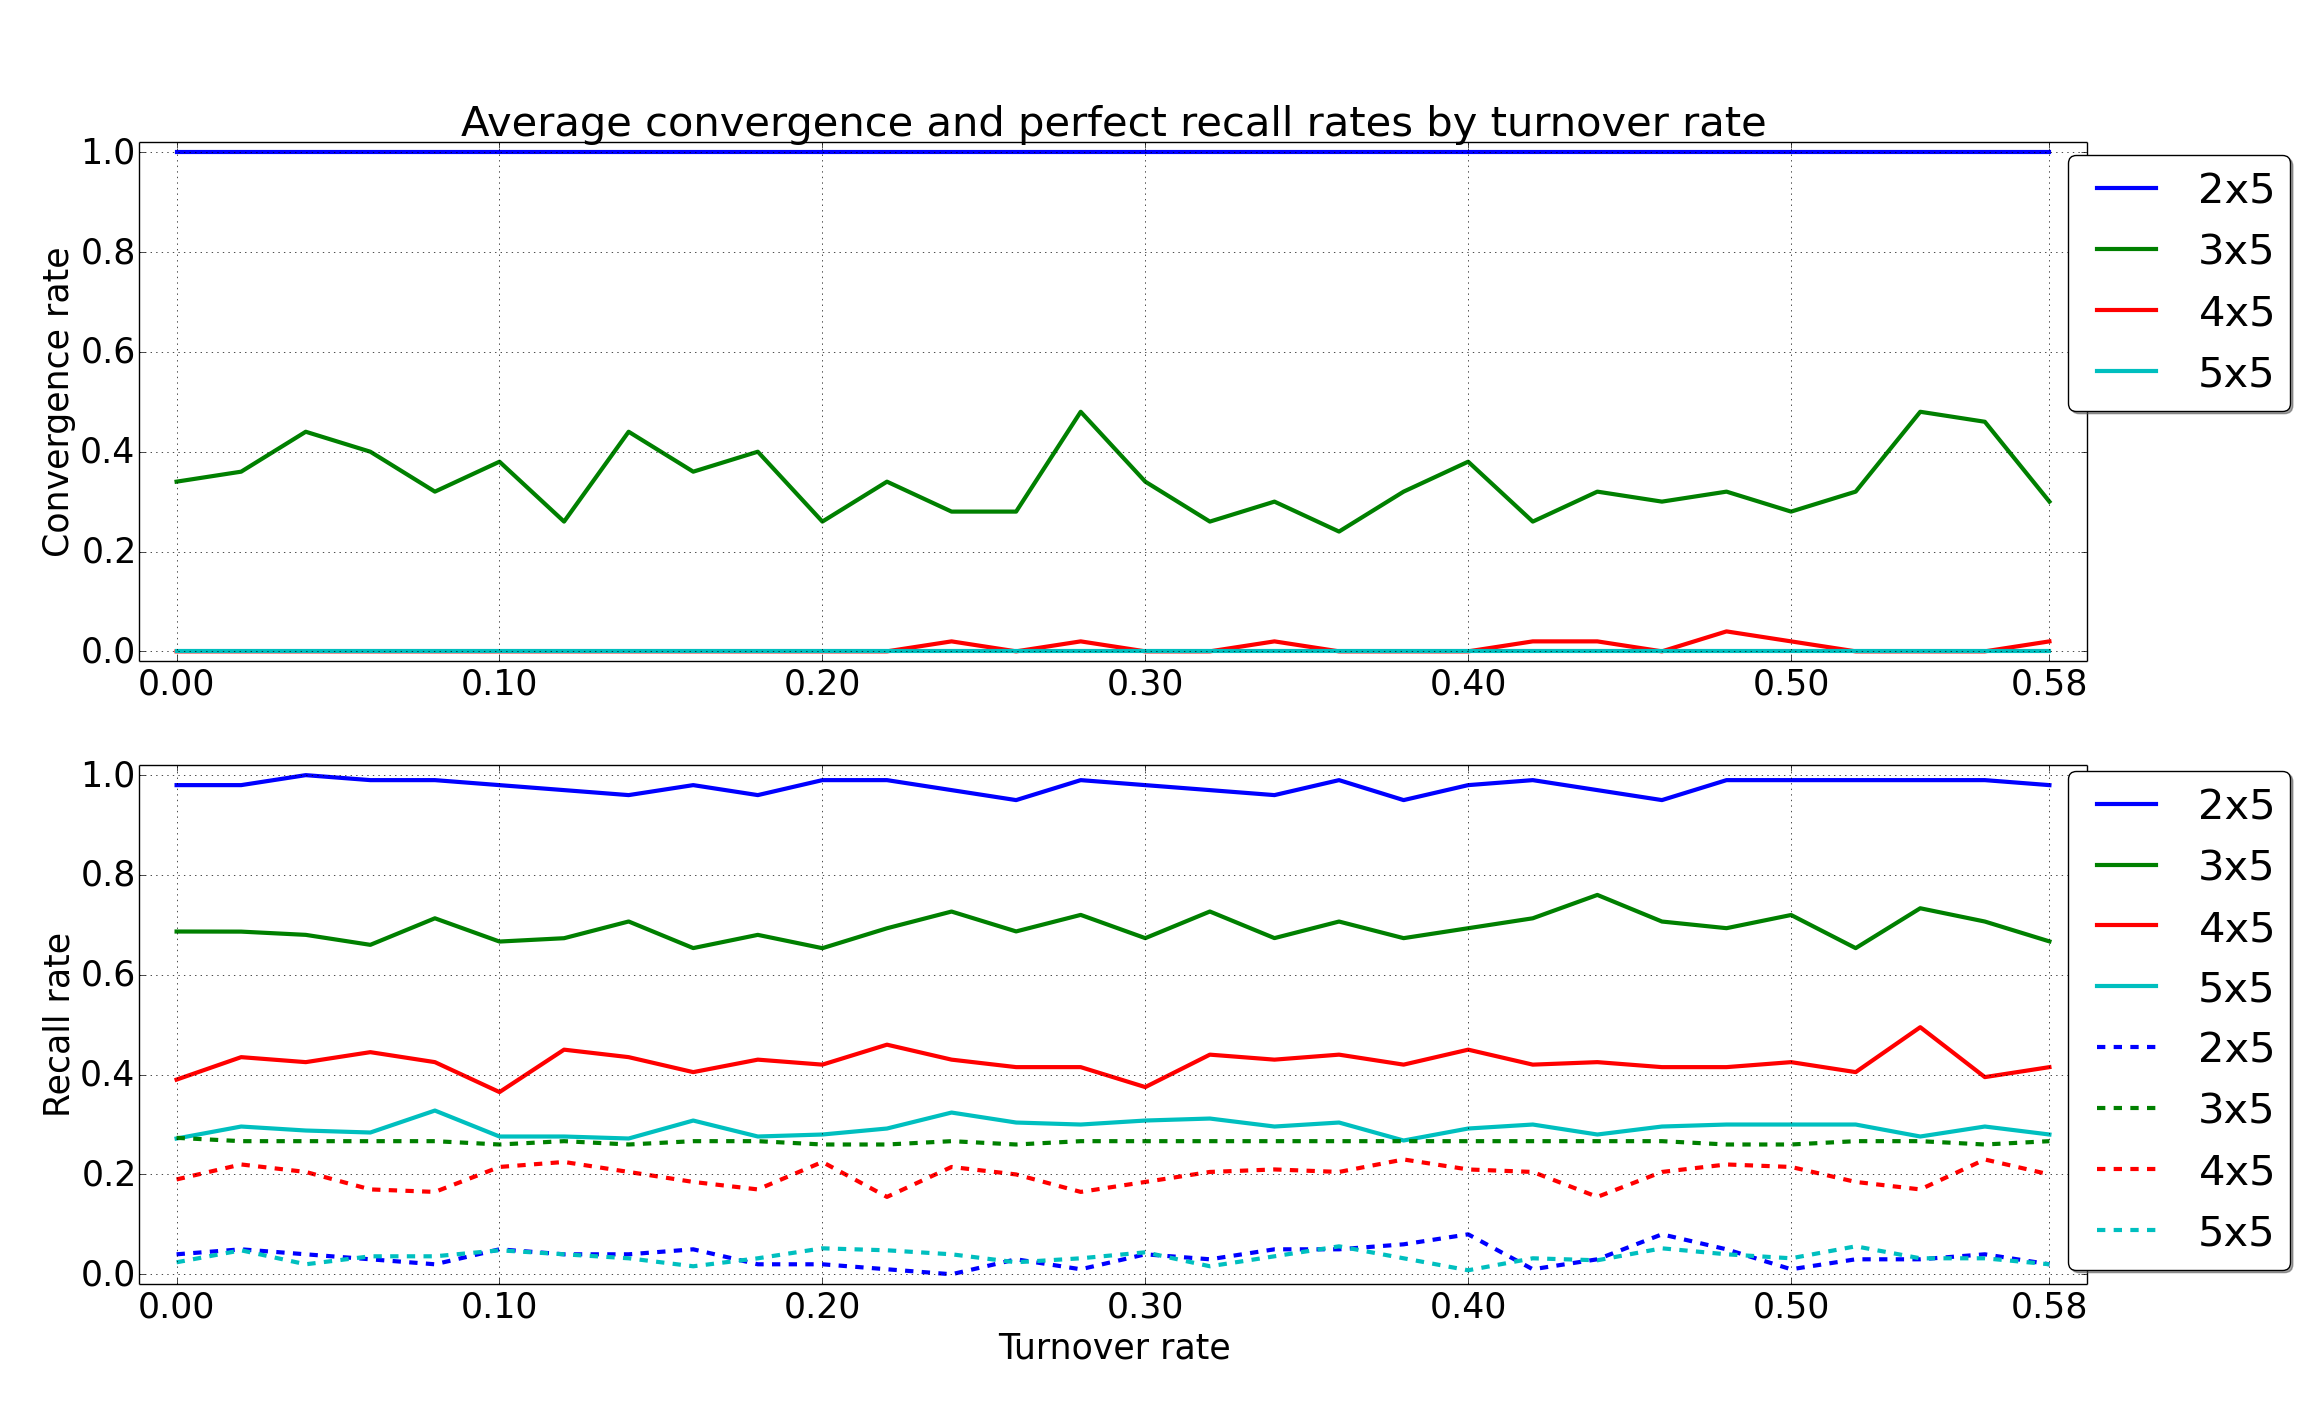
\includegraphics[width=13cm]{fig/turnover_rates/async_tm0_dgw1}
    \caption{Displaying the average \textbf{convergence rate (upper graph) and perfect and spurious recall rates (lower graph) by the neuronal turnover rate}. In this figure the model employs asynchronous CA3 neuron-updates, with neuronal turnover being performed between every learnt training subset, and a DG-weighting of 1. Note that the perfect recall rate seems unaffected by a changing turnover rate.
    Average convergence by neuronal turnover rate, for asynchronous CA3 neuronal updating, and turnover between every learnt training (sub-)set. Note that convergence seems unaffected by a changing turnover rate.}
    \label{fig:async_tm0_dgw1}
\end{figure}

Figure \ref{fig:async_tm0_dgw1} raises the question of whether the model contains any issues related to the DG-layer, as the layers' parameters do not seem to affect model performance. Because highly similar results were attained for all three neuronal turnover configurations when using asynchronous CA3-layer updating, figures for the two remaining asynchronous model schemes are contained in appendix D.
It may be that the asynchronous CA3-layer updating scheme introduces a certain robustness to the model, seeing that permuting and re-instantiating a large number of the EC-DG and DG-CA3 synapses for every training set iteration does not reduce the model performance. 
However, the convergence rates indicate poor convergence in all scenarios. Furthermore, when investigating the figures (\ref{fig:sync_tm0_dgw25}, \ref{fig:sync_tm1_dgw25}) for synchronous CA3-neuron updating, neuronal turnover rate does in fact positively impact the perfect recall rates of the model when the DG-weighting is set to $25$.

\begin{figure}
    \centering
    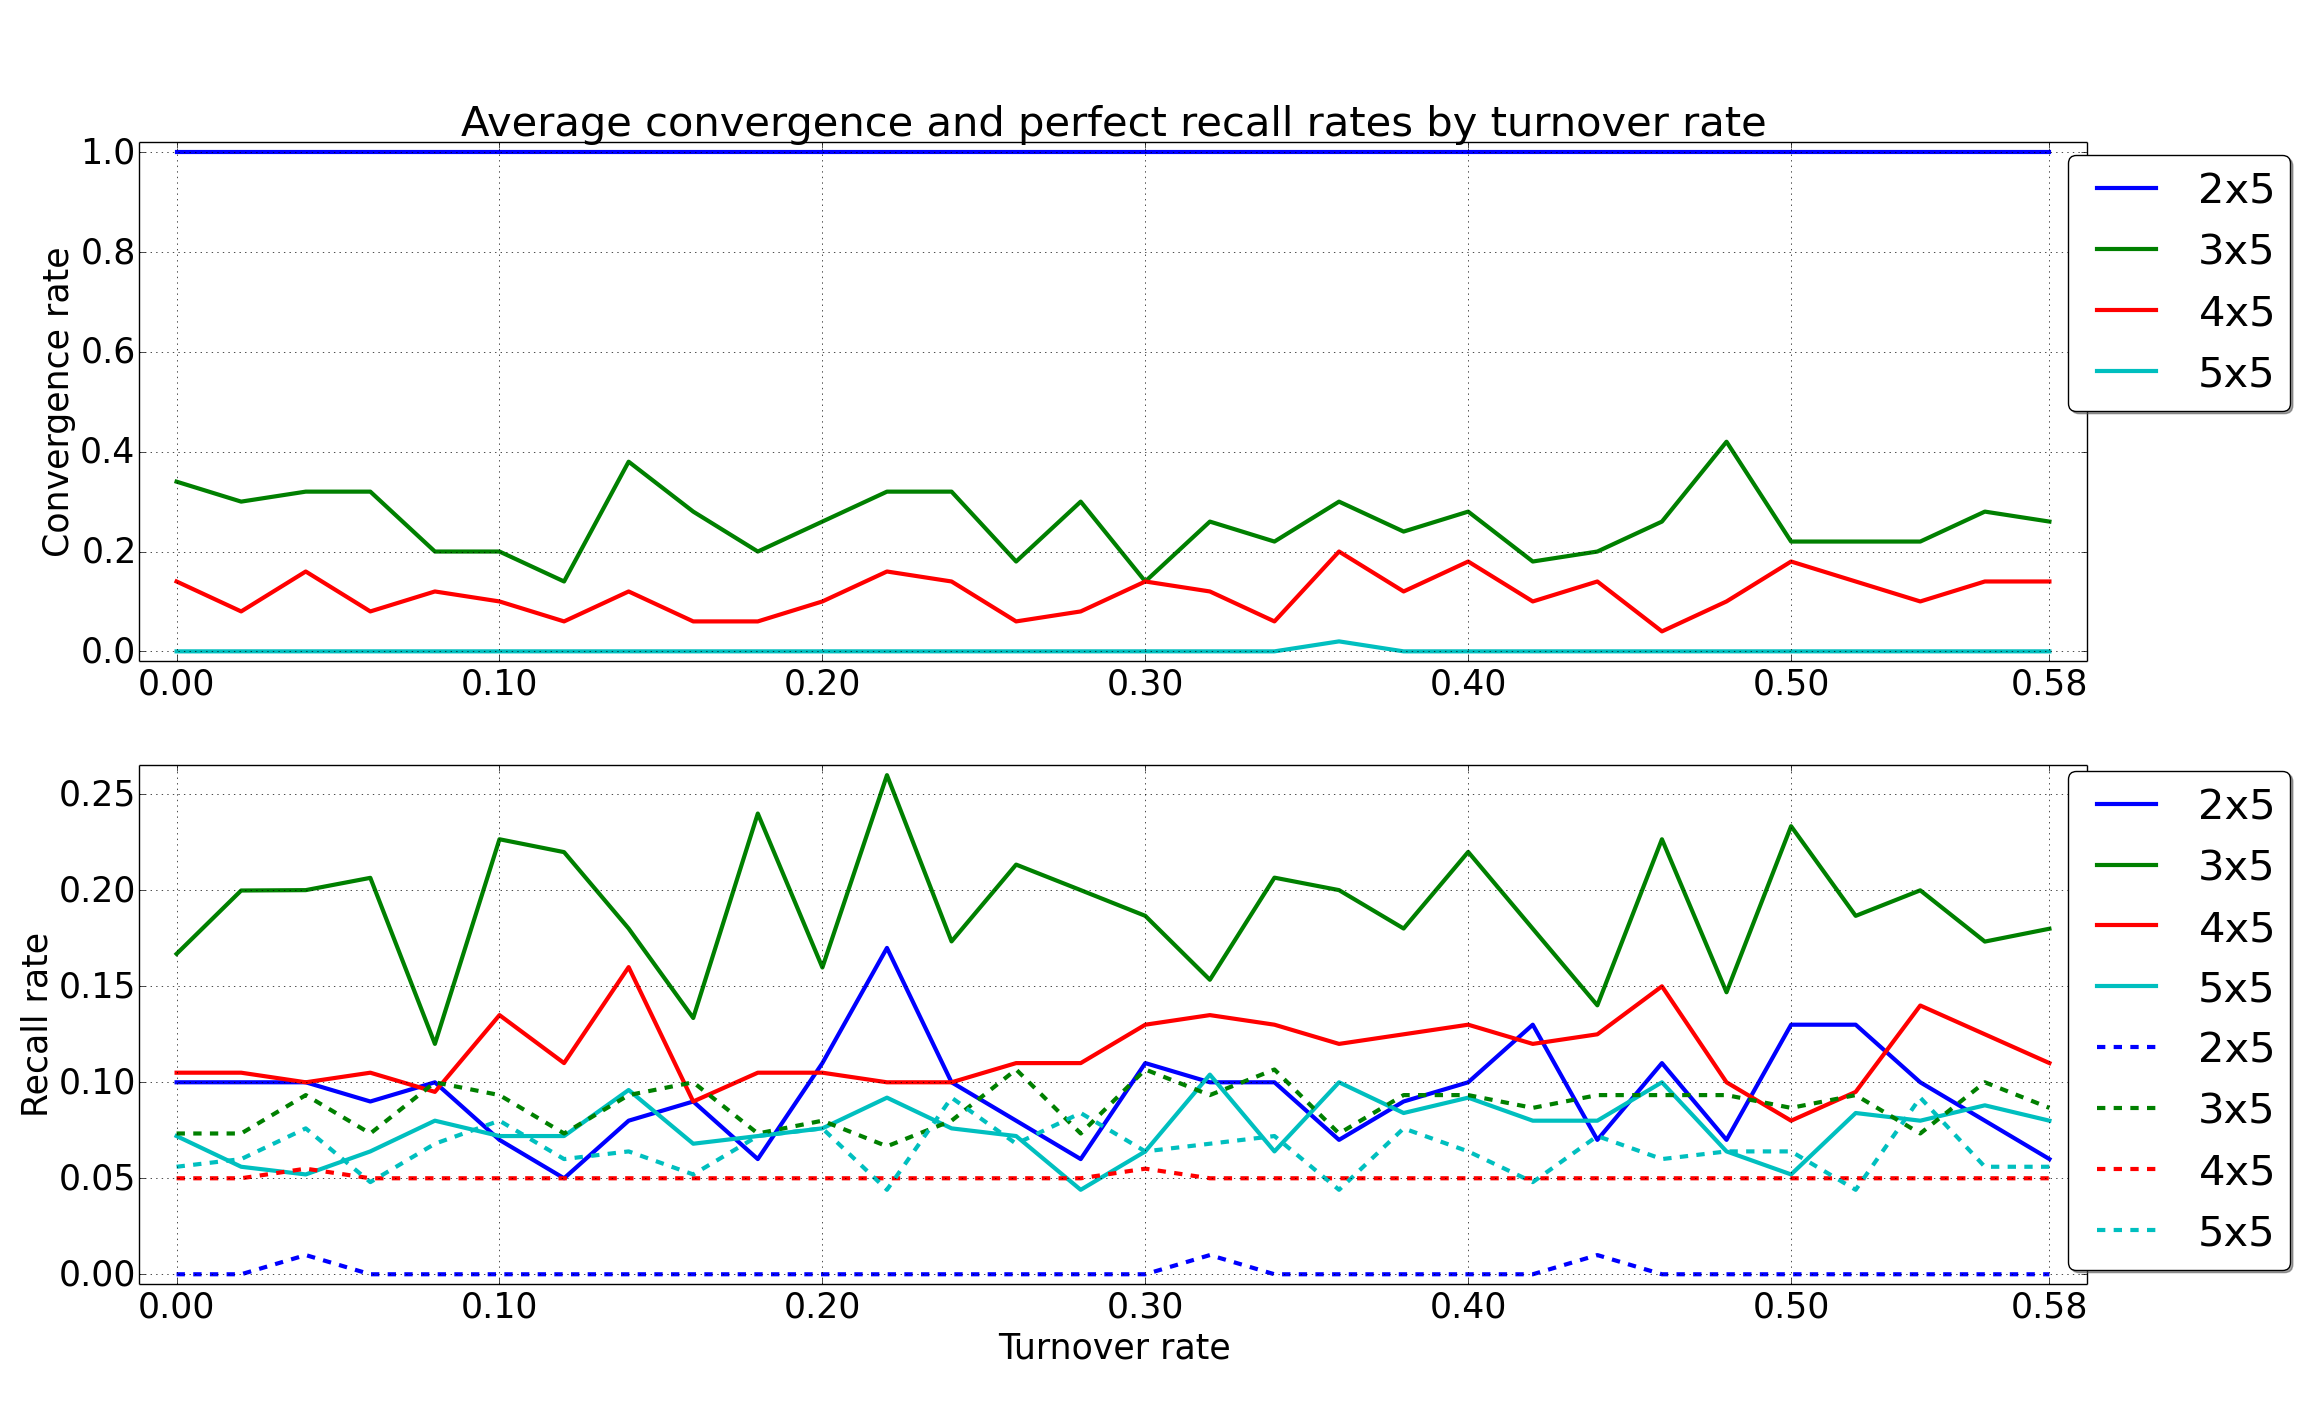
\includegraphics[width=13cm]{fig/turnover_rates/sync_tm0_dgw1}
    \caption{Illustrating the \textbf{average model convergence and recall rates by neuronal turnover rate} for synchronous CA3-layer updating, using a DG-weight coefficient of 1, and neuronal turnover between every learnt training subset. Note that the model seems to largely fail to converge for any set size other than 2x5, which may indicate that pattern separation is unsuccessful, which would also explain why changing the neuronal turnover rate does not affect the model performance in figure \ref{fig:async_tm0_dgw1}.}
    \label{fig:sync_tm0_dgw1}
\end{figure}

Model convergence is not attained in the synchronous CA3 neuronal updating scheme when a DG-weighting of 1 is employed, with the perfect recall rate remaining poor. This suggests that the model is both unable to separate the patterns for the correct input patterns during learning and recall when the DG-weighting is 1.
Note that when increasing the DG-weighting to 25, the model converges for 80-100 \% of the training patterns, irrespective of set size. Further, this results in perfect recall rates of twice as high values, suggesting that increasing the connection weighting of the synapses from the DG-layer to the CA3-layer may in fact enable pattern separation during learning and chaotic recall. 
Note that the neuronal turnover rate seems uncorrelated with model performance when performing neuronal turnover between learnt subsets. Interestingly, when performing neuronal turnover for every training iteration (DG-weighting $= 25$, synchronous updating), results in the best model performance attained so far. Namely in  nearly 80 \% of the training sets from the 3x5 auto-associative training set being perfectly recalled for $\tau\in\approx[0.40, 0.58]$.
Furthermore, there is a slight increase in the recall capability during learning of the other set sizes too. It is important to emphasise that while perfect recall increases significantly for higher turnover rates, with the highest rate in the aforementioned interval; so does spurious pattern recall. While such low spurious recall rates may be acceptable, strict convergence is only attained for sufficiently low turnover rates. Interestingly, the figure suggests that rather high turnover rates may be used while not spuriously recalling patterns (such as $\tau=0.30$). Furthermore, note that some patterns are spuriously recalled for very low turnover rates. This suggests that when the turnover is too low, pattern separation is unsuccessful.
Shortly put, figures \ref{fig:sync_tm0_dgw25} and \ref{fig:sync_tm1_dgw25} elucidate pattern separation in the outlined model, demonstrating that a certain level of continuous turnover is preferable for successful pattern separation, and further suggesting that employing strongly connected synapses in the DG-CA3 pathway enables pattern separation altogether.

\begin{figure}
    \centering
    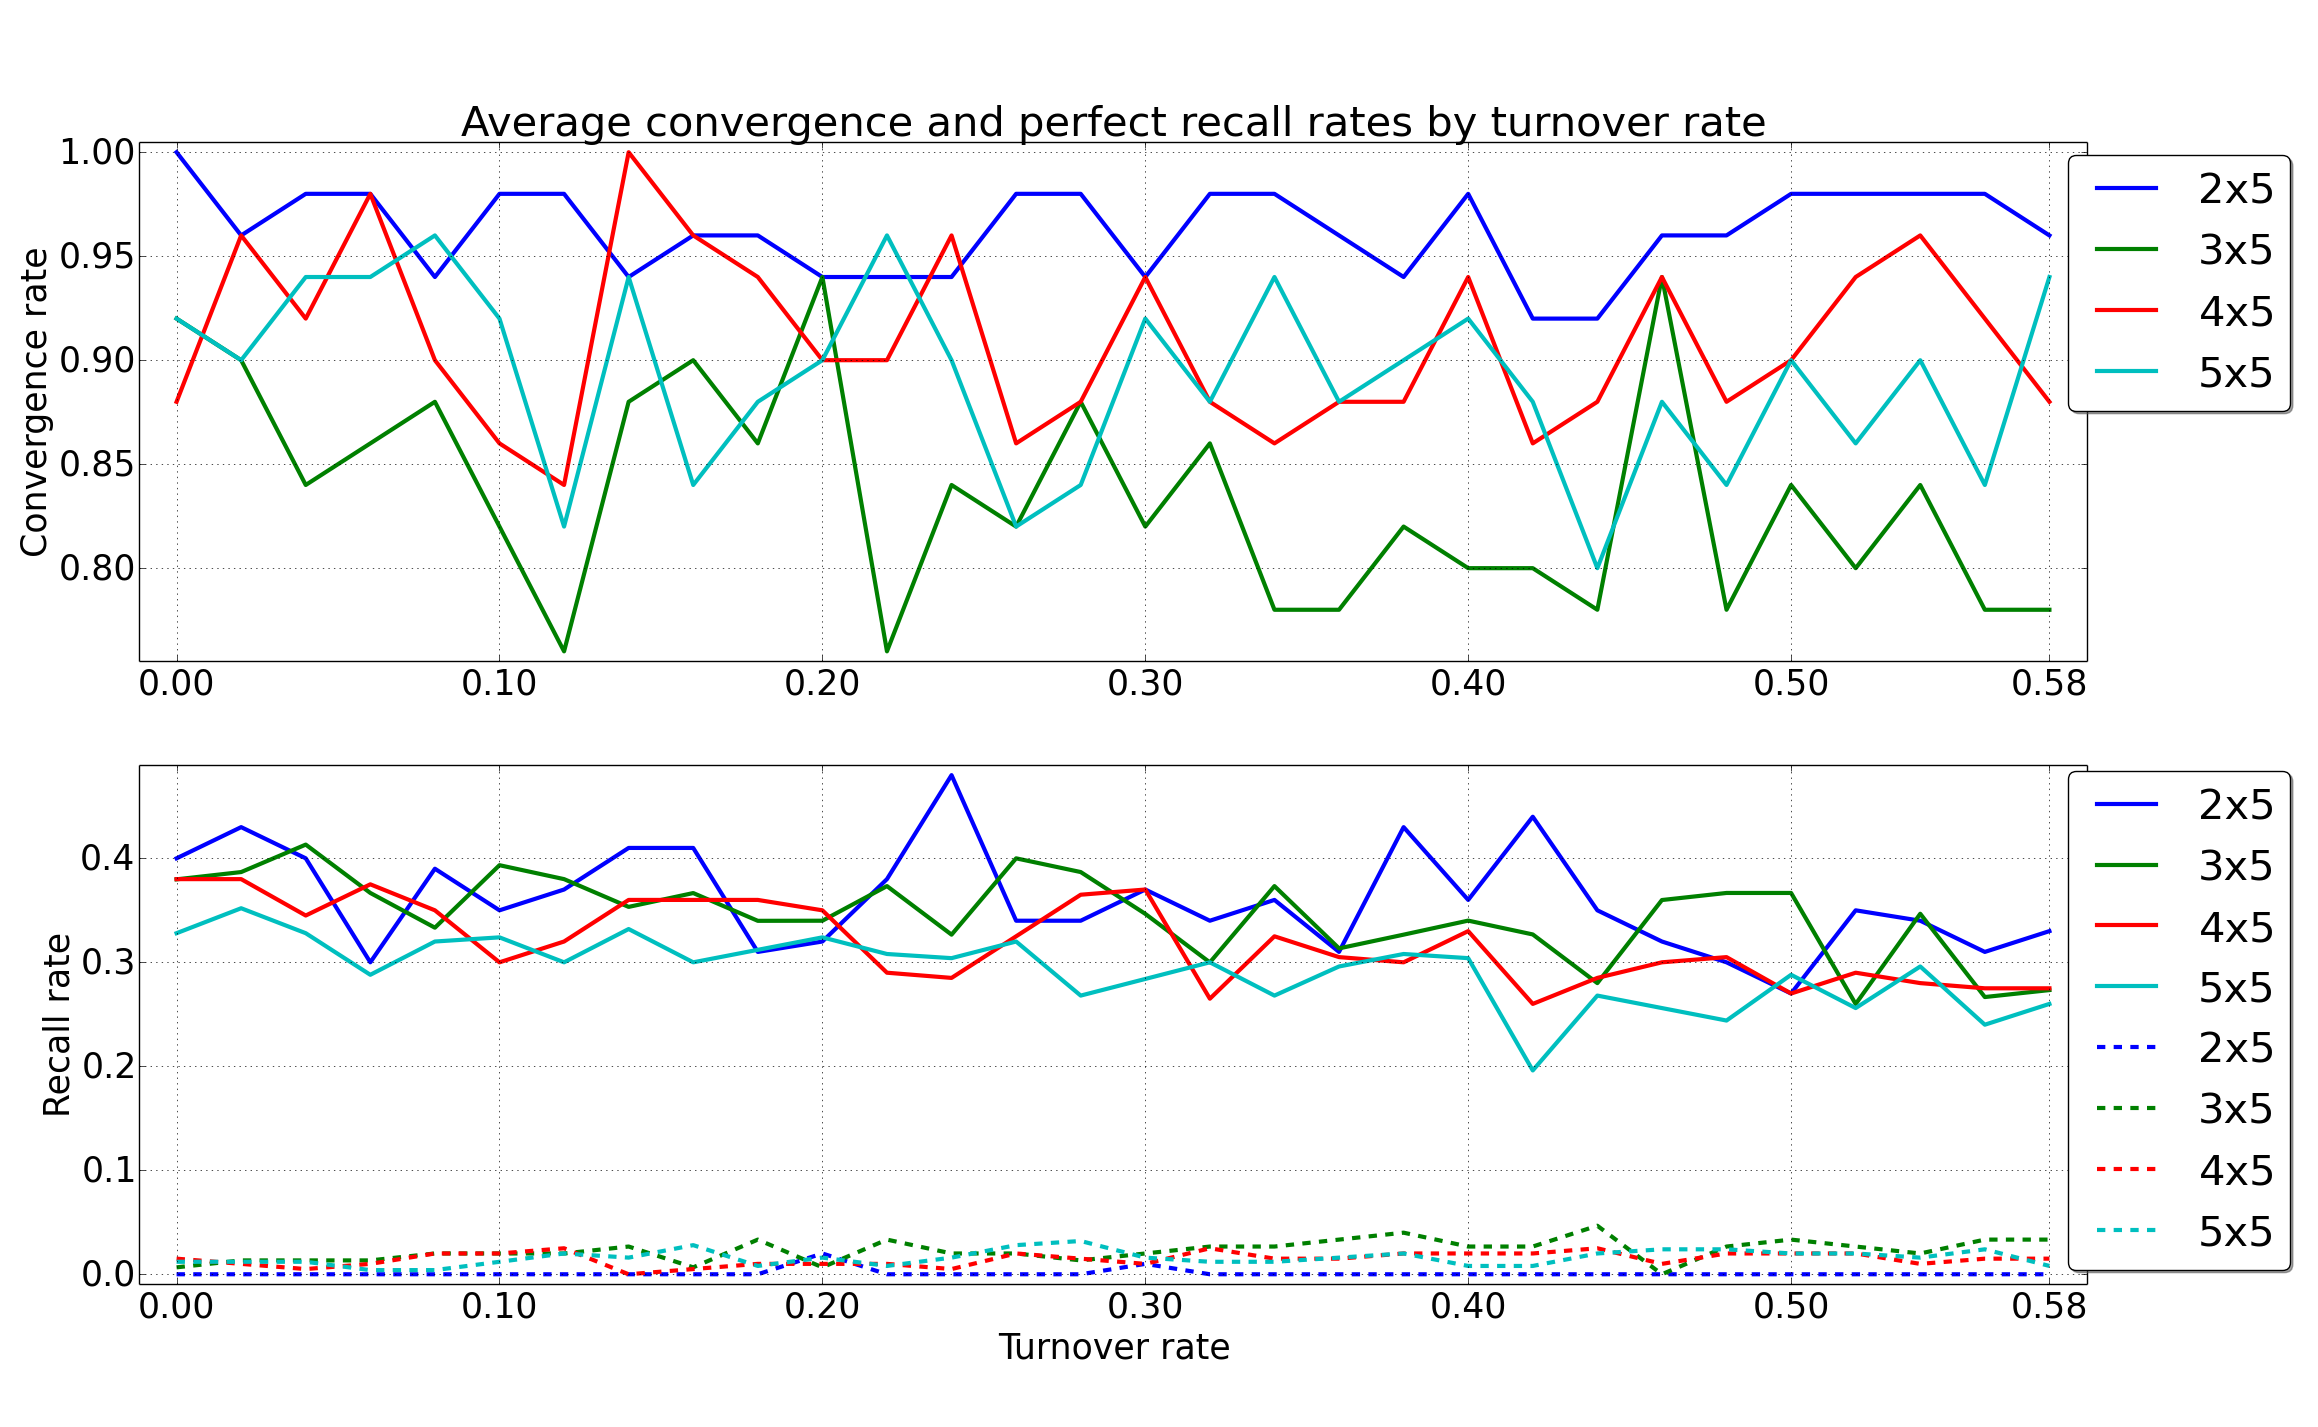
\includegraphics[width=13cm]{fig/turnover_rates/sync_tm0_dgw25}
    \caption{Presenting the \textbf{average perfect recall rate by neuronal turnover rate} for the scheme of synchronous updating, now using a DG-weighting of 25, turnover being performed for every new training subset. Note that neuronal turnover does not seem to affect model performance significantly. However, there is a slight tendency towards a worse perfect recall rate as the turnover rate grows towards 0.50.
    Convergence is attained in about 80 to 100 \% of the cases, but is not correlated with the training set size.}
    \label{fig:sync_tm0_dgw25}
\end{figure}

\begin{figure}
    \centering
    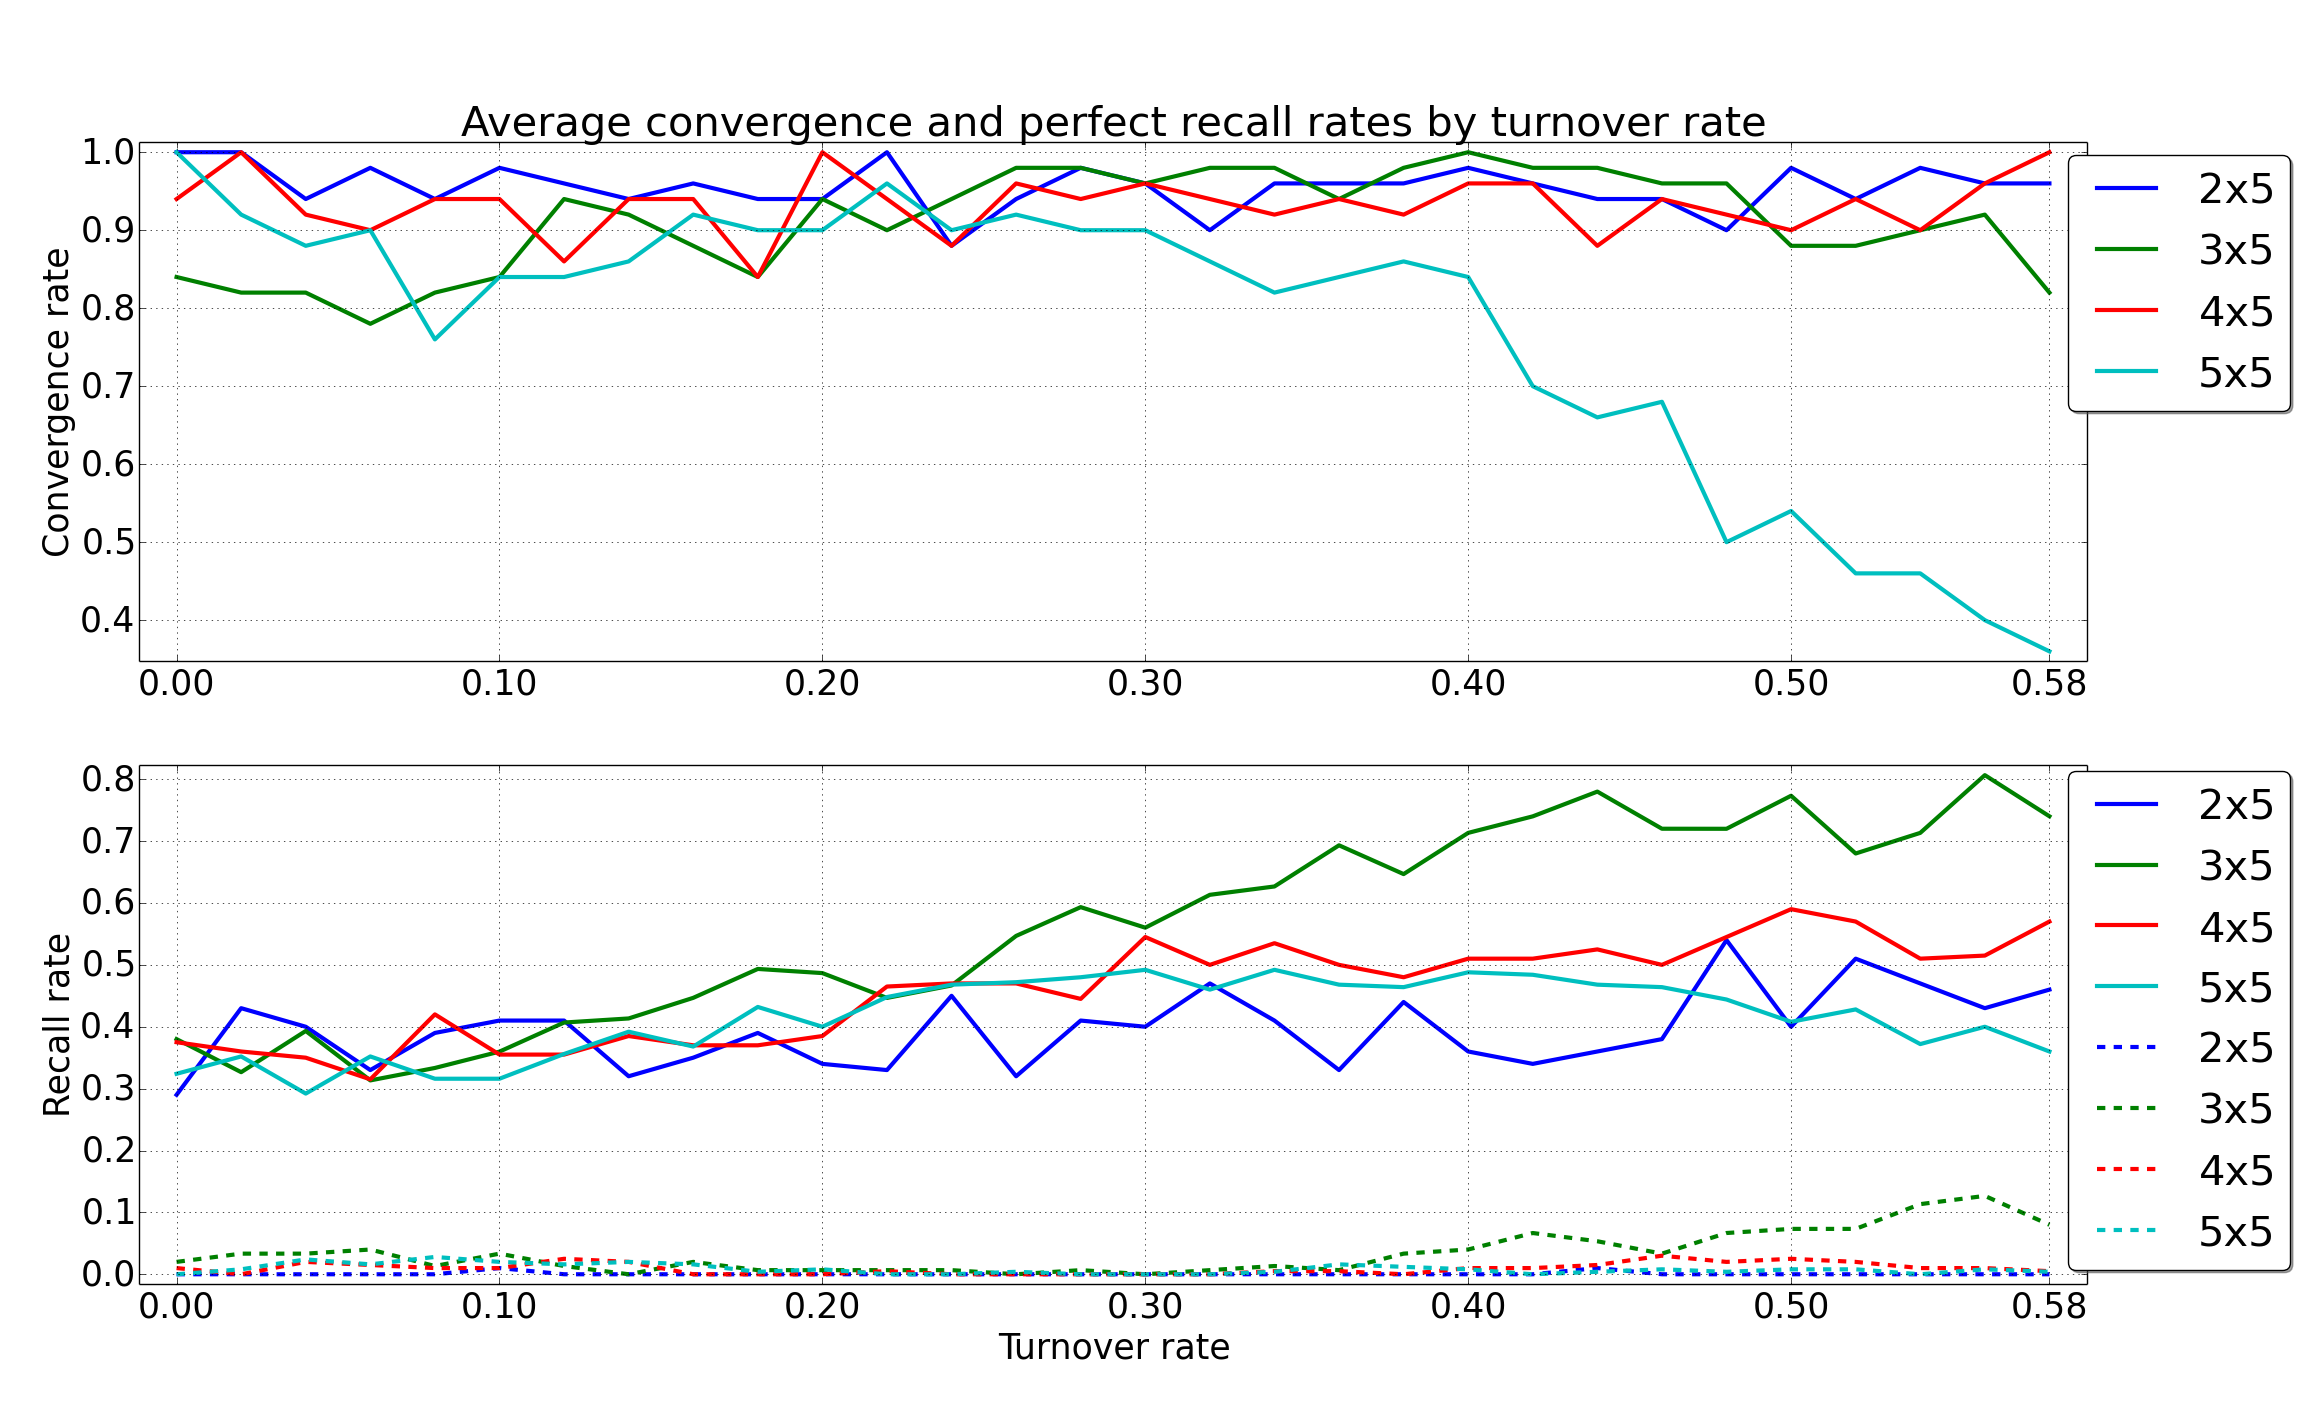
\includegraphics[width=13cm]{fig/turnover_rates/sync_tm1_dgw25}
    \caption{Showing the \textbf{average perfect recall rate by turnover rate} for the scheme of synchronous updating with a DG-weighting of 25, turnover being performed for every training iteration. Interestingly, model performance is now highly correlated with the turnover rate, when turnover is being performed very frequently.
    Convergence is attained in about 90 to 100 \% of the cases, and seems to be best for a neuronal turnover rate $\tau$ in the interval of approximately $[0, 30]$. Note that the convergence drops rapidly for the largest training set size when $\tau$ goes above this value (for $\tau \in [0.30, 0.58]$).}
    \label{fig:sync_tm1_dgw25}
\end{figure}

As asynchronous neuronal updates use the newest updated values in the CA3-layer through its recurrent connections, this may in fact introduce too much randomness in the model. One solution to this may be to introduce hardware-mediated asynchronicity through algorithmic parallelization, as this is more likely to mainly use the current neuronal values, thus largely reducing the randomness and the combinatorial explosion of the outcome space during neuronal updating and wiring. This reduction is somewhat relaxed, enabling a trade-off of yet maintaining a certain randomness to the model. Furthermore, this scheme is may be more biologically realistic, as updating in the biological brain is performed continuously and only slightly synchronously (and at different time-scales). However, both implementing and elaborating more on such a scheme remains outside the scope of this thesis.

Note the successful increase in perfectly recalled patterns for set size 3x5, but not 2x5 when increasing the neuronal turnover rate in the synchronous CA3-updating scheme using turnover for every training iteration, figure \ref{fig:sync_tm1_dgw25}. Because both patterns are successfully recalled when the correct corresponding input is present in the 2x5 training scheme, but not during recall, this suggests that one of the patterns in the 2x5 scheme covers most of the weight space, thus being the only pattern which is reached during learning. Furthermore, increasing the number of patterns also necessarily increases the need for pattern separation in order for the model to converge. Therefore, each pattern is more likely to occupy more of the weight space, thus increasing the area of its basin of attraction (i.e. the area inside which the network will converge towards the output pattern). Additionally, figure \ref{fig:sync_tm0_dgw25} demonstrates that when turnover is only performed between training sets, increasing the turnover rate only slightly decreases the perfect recall rate. This suggests that while increasing the frequency of performing turnover to every training iteration may provide the model with more randomness, expanding the model's search through learnt patterns, it only slightly improves the recall capabilities. Furthermore, expanding the search space also introduces some more spuriousness to the recall process. This provides the basis for the next experiments, where the convergence criterion is designed to be less stringent, as well as to potentially assign patterns more evenly in the model's weight space.

% ======================= exposure schemes ========================
\subsection{Experiment 4: Relaxing the convergence criterion}\label{sect:relaxed-criterion}

Because the results presented above in experiments 1-3 indicate issues related to chaotic recall, these experiments investigate how reformulating and relaxing the convergence criterion may impact model behaviour. Convergence is now considered to be attained once a static number of training or recall iterations have been performed. In this experiment the number of iterations is set to 15 as the criterion during recall, and 15 for most of the experiments during training, based on empirical data from previous experiments.
Although the model is shown to be capable of one-shot learning in the low-level demonstration contained in the first parts of this chapter, convergence is only attained in less than 15 training iterations for set size 2x5 in the introductory experiments using the stringent convergence criterion (of stable output for three recall iterations). On average, the synchronous CA3 updating mode converged in 2-3 training iterations, which demonstrates a clear one-shot learning capability, while the in the asynchronous mode it converged in on average about 7 iterations for training set size 2x5. 
%
% Interestingly, these ranges are very similar to those thought to be required (approximately) for human subjects to learn new training sets \citep{Rolls1998chpt6} [double-check].
Nevertheless, as the set size grows larger, i.e. 3-5 per subset, the number of required training iterations grows slightly larger than 15 for the synchronous CA3 updating mode (approximately 20 for the remaining set sizes), and linearly towards 50, i.e. no convergence at all for the asynchronous CA3 updating mode.
While convergence thus may not be attained for 15 training iterations according to the previous learning criterion, the model will definitely have had time to be completely exposed to the new training subset, adapting its weights accordingly (to the subset). Furthermore, 15 iterations is also more than sufficient in order to have former short-term memory diminish, as may be seen in the low-level example figures contained in appendix D.
However, 50 iterations during training is also used in some of the experiments in order to investigate the potential effects this has on model performance and the quality of extracted patterns.

What I wish to investigate in this experiment are the trends that may arise under a more constant training scheme. Even though convergence is not strictly attained, the number of iterations does allow for learning pattern associations. Furthermore, exposing the model to a constant and uniformly distributed continuous flow of patterns is more likely to generate trends that are representative of model behaviour, both during recall and learning. As such, observing trends for a more static scheme may ameliorate the unsuccessful chaotic recall that is observed under the more stringent chaotic recall scheme and convergence criterion. Thus, observed trends may in fact provide a better picture of the model behaviour, and the observed trends may potentially help further illuminate the research questions, as well as the pattern separation aspects related to synchronicity and neuronal turnover that remains slightly obscure from previous experiments and results.

% \subsubsection{Local training set exposure}

\begin{figure}
    \centering
    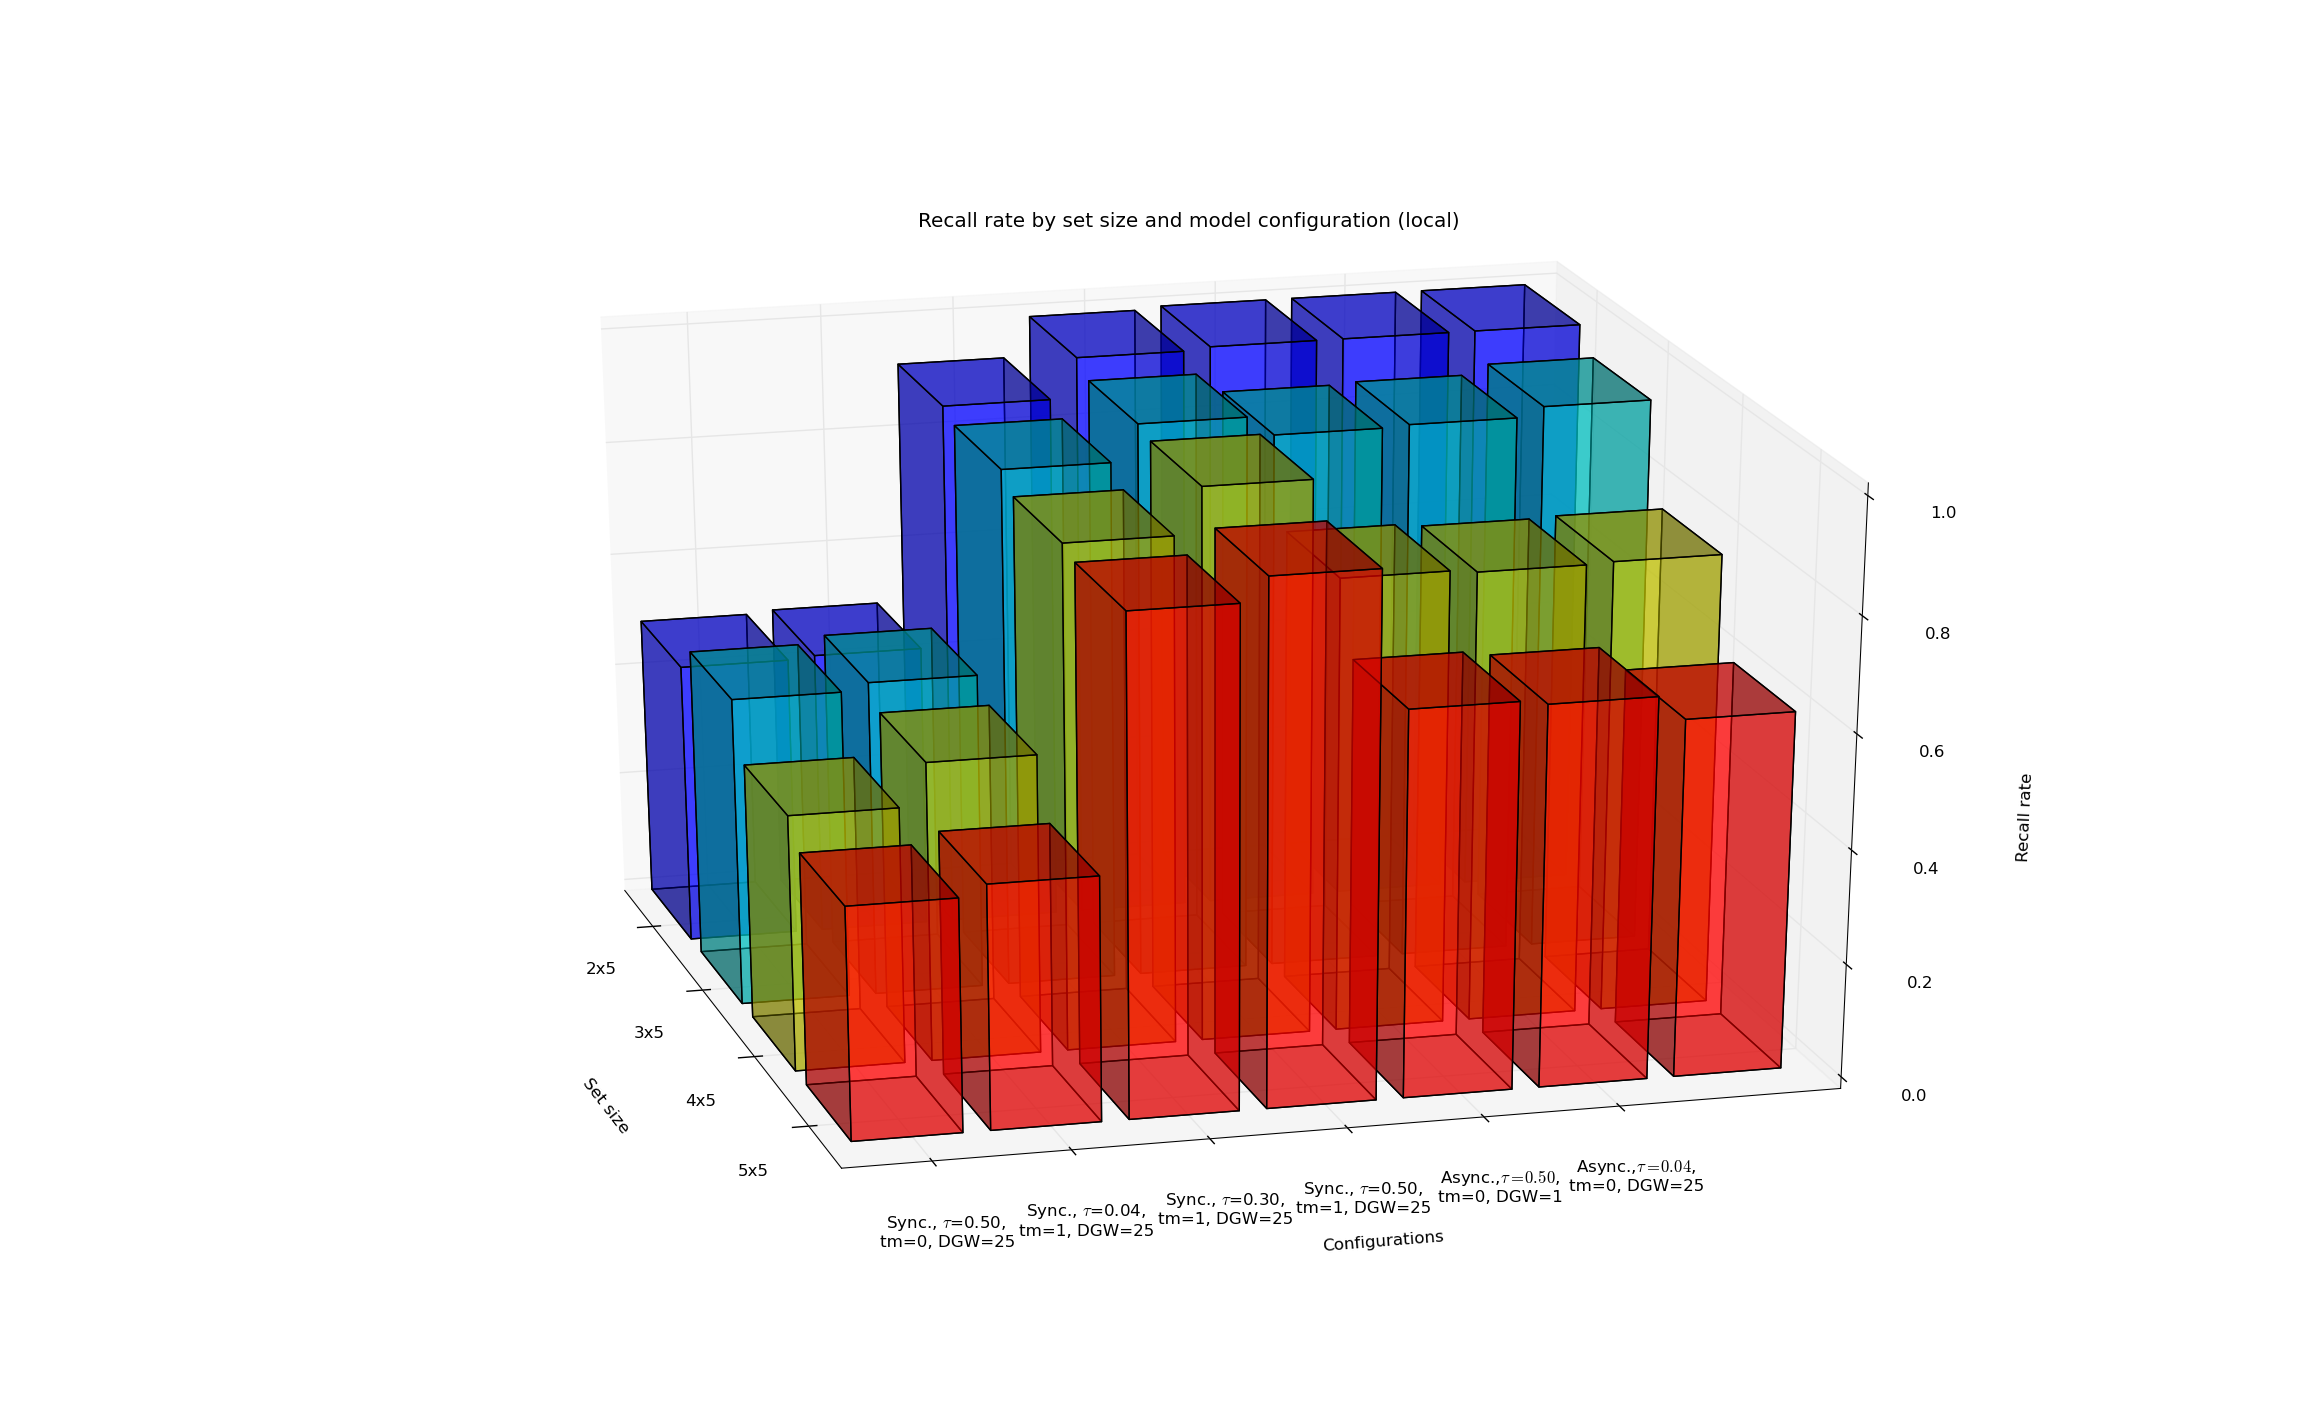
\includegraphics[width=14cm]{fig/i-iters/local-recall}
    \caption{Perfect recall rates in several hippocampal model schemes for both synchronous and asynchronous CA3-layer updating, the \textit{'local'} keyword in the title denoting that the models are trained on each subset of the corresponding set sizes, sequentially. Note that performing turnover for every training iteration seems to enhance the perfect recall rate when using synchronous CA3-updating significantly. However, this does not seem to have an effect for low turnover rates, such as $\tau=0.04$, nor under asynchronous updating schemes. Note also that "tm=0", and "tm=1", denotes that neuronal turnover is performed between every learnt training subset, or for every training iteration, respectively.}
    \label{fig:local-recall}
\end{figure}

\begin{figure}
    \centering
    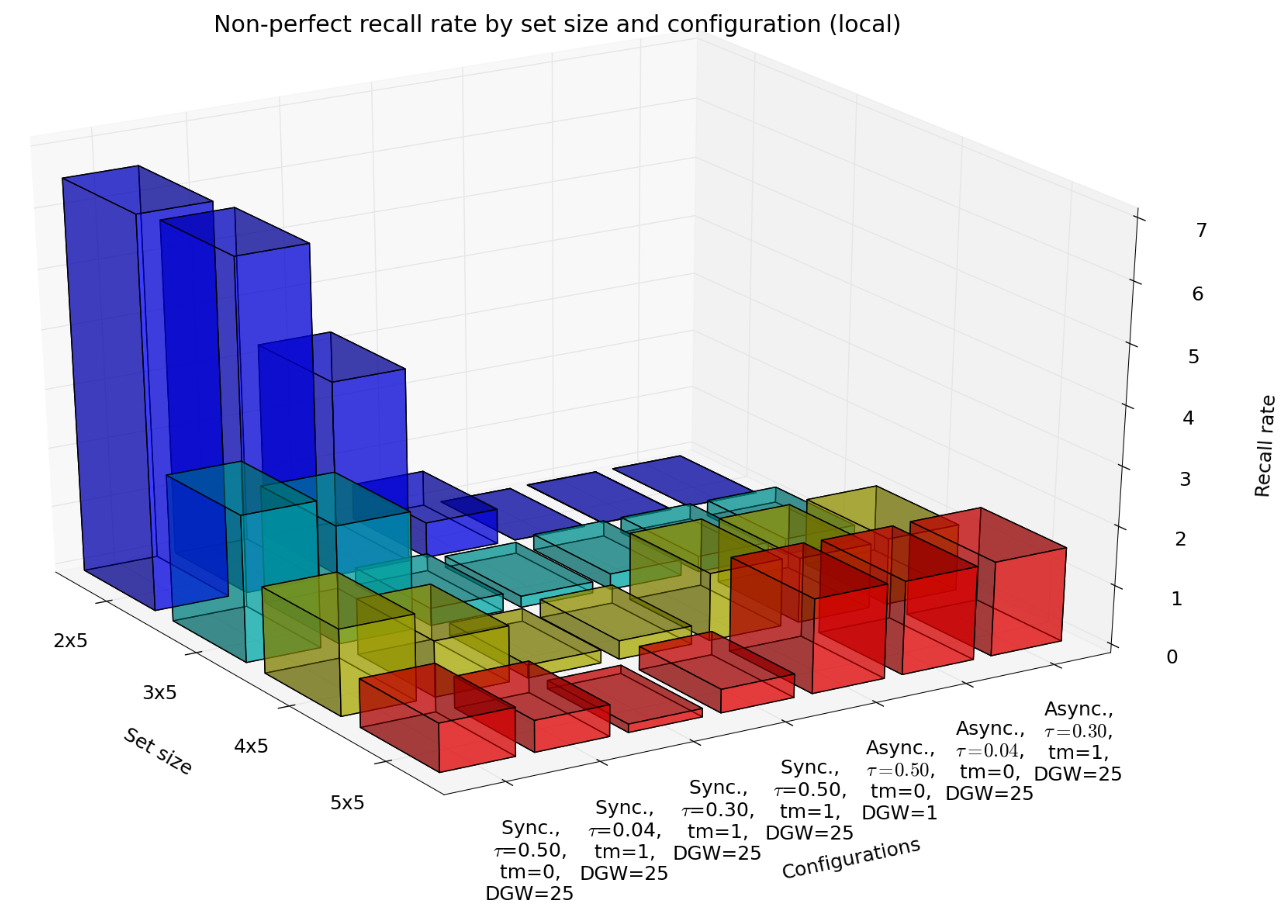
\includegraphics[width=14cm]{fig/i-iters/local-recall-spurious}
    \caption{Displaying the spurious extraction rates corresponding to the perfect recall rates and model schemes of figure \ref{fig:local-recall}, for local recall, i.e. training on subsets sequentially.}
    \label{fig:local-recall-spurious}
\end{figure}

Note that while perfect recall by chaotic recall is significantly better for synchronous rather than asynchronous CA3 updating in the global training set exposure scheme, the results are slightly worse than in the local exposure scheme. Furthermore, in the local exposure scheme, the asynchronous updating modes perform slightly better than the synchronous, despite the DG-weighting being 1. This may demonstrate a limited pattern separation ability of the model in the asynchronous CA3 updating schemes. However, the fact that performance is lowered very little in the synchronous scheme suggests and demonstrates that the model configuration is capable of fairly robust pattern separation.

% \subsubsection{Global training set exposure}
\begin{figure}
    \centering
    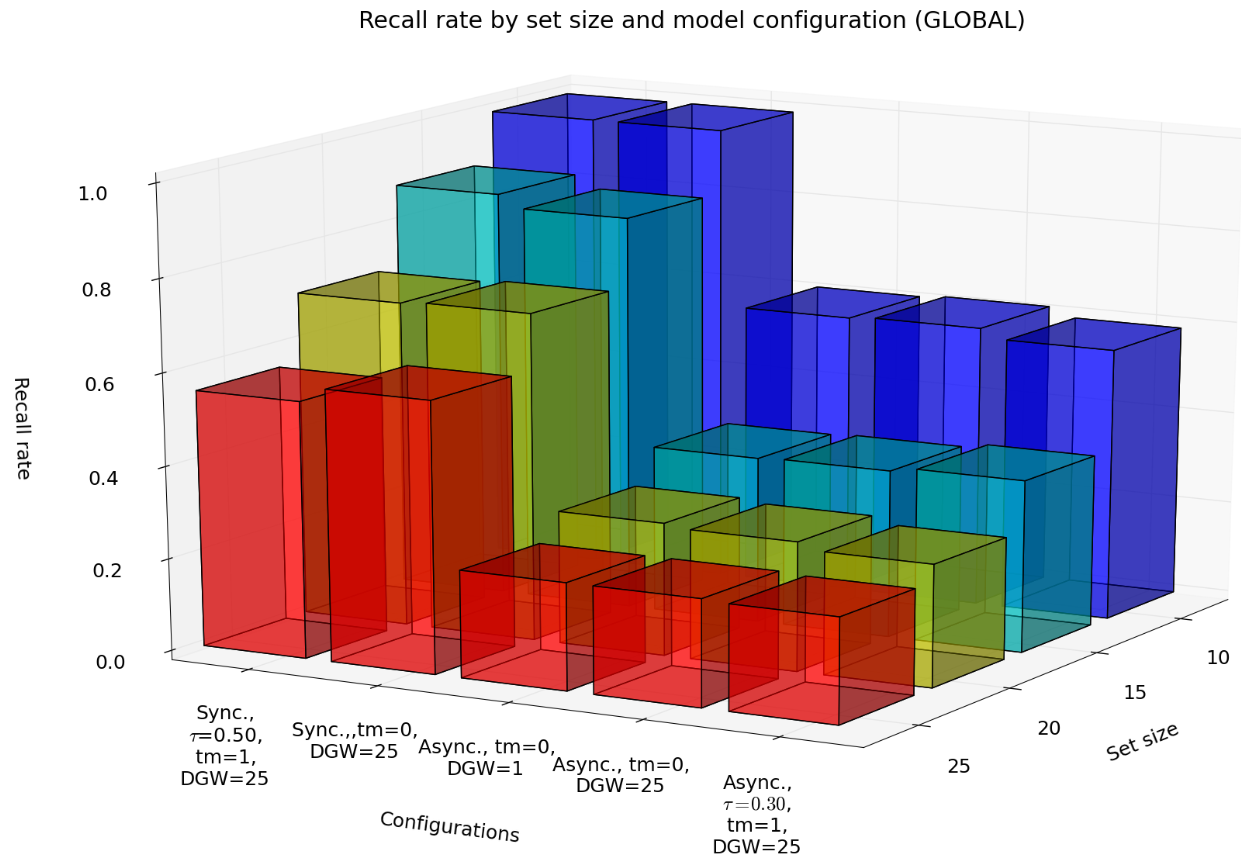
\includegraphics[width=13cm]{fig/i-iters/global-recall}
    \caption{Displaying the \textbf{perfect recall rates under global training set exposure} attained for five different model schemes when the hippocampal model is exposed to all of the training patterns.}
    \label{fig:global-recall}
\end{figure}

\begin{figure}
    \centering
    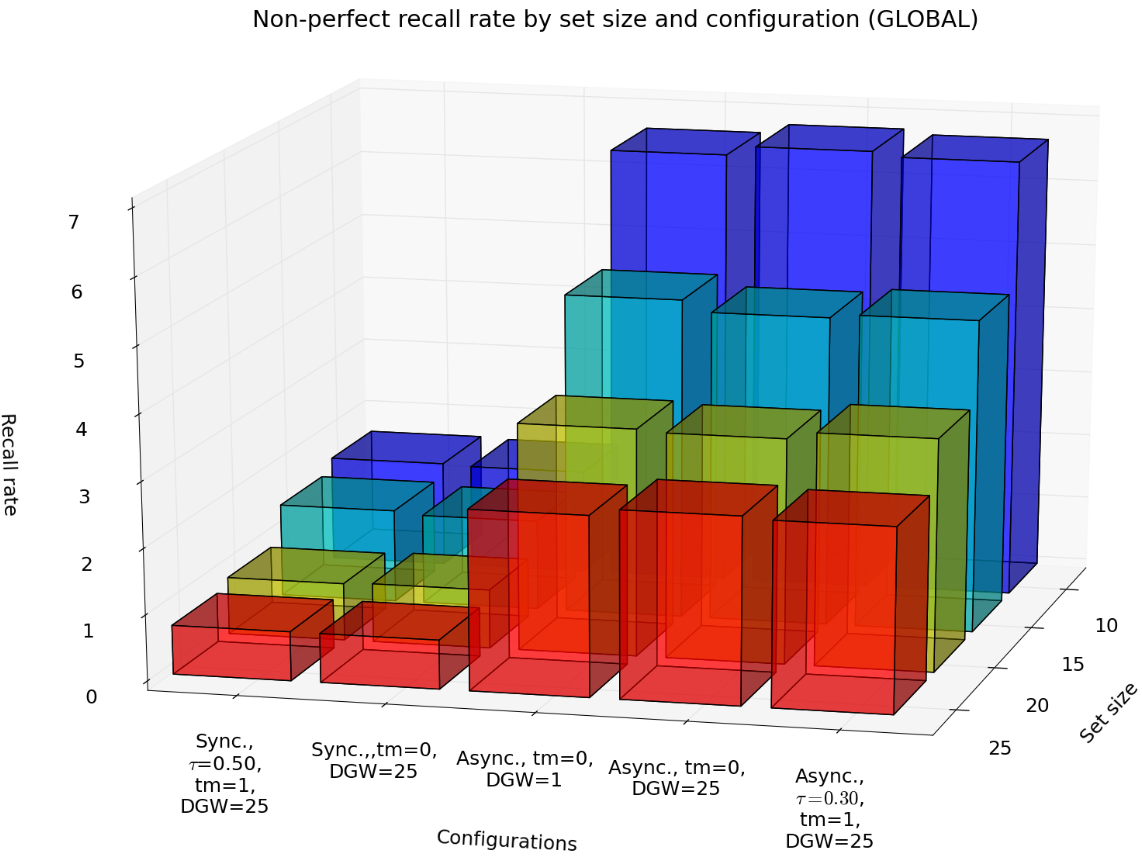
\includegraphics[width=13cm]{fig/i-iters/global-spurious-recall}
    \caption{Displaying the \textbf{chaotically extracted spurious patterns for global training set exposure} under several model schemes.}
    \label{fig:global-recall-spurious}
\end{figure}

It is worth noting that the synchronous CA3 updating scheme results in a relatively large number of spuriously recalled patterns for small set sizes. This may in indicate that the learned patterns' basins of attraction have merged, corresponding to spurious pattern(s) which may then be learned by the model. As previous empirical data, as well as the low-level demonstration has shown that the model on average successfully recalls patterns for the correct pattern input, this may point towards the issue residing within the synchronous updating schemes' recall procedure. 
Note however that once the model fails to separate two similar patterns and forms a novel spurious pattern and basin of attraction, this basin may increase the likelihood of further such spurious basins being created. This may be seen by considering that such a basin is in fact an overlap between the other basins, which is then likely to contain parts of other patterns and letters, too. In this case, the overlapping inputs will necessarily disrupt the pattern-completion of the CA3-layer, as it cannot settle into patterns that overlap too much. This phenomena has been demonstrated in work on auto-associative networks, as discussed in the background chapter, as well as in \citep{Hattori2014}, which employs a more complex HPC-model specifically to alleviate the issues of pattern separation and memory congestion in a simple Hopfield network, as is used in \citep{Hattori2010}.
Looking to the low level demonstration of the synchronous training and recall scheme, a fair stability is attained for learned pattern inputs, however, chaotic recall seems to be very unstable, only visiting learned pattern outputs for one time-step. In other words, the \textit{correct} basins of attraction have not been sufficiently consolidated for the given letters, as the output oscillates. Whether consolidation is unsuccessful due to the creation of basins of attraction for spurious pattern correlations, or only because pattern separation is unsuccessful - which necessarily renders successful learning and convergence unsuccessful, remains slightly obscure. That being said, the chaotically recalled output seems to recur only for the actual training pattern output, with spurious chaotically recalled patterns only occurring once per spurious pattern. This suggests that chaotic recall is unsuccessful largely due to unsuccessful reduction in overlap of the training patterns. One thing that could ameliorate this issue is introducing a slight neuronal turnover for every training set iteration, although less biologically realistic. If successful, it could however imply that the biological brain needs a certain randomness to its learning procedure in order to enhance its correlation extraction. This could also be more biologically realistically implemented by introducing random "noise" in between training patterns, which would introduce randomness in the eta- and zeta-equations, and thus to the chaotic neurons of the CA3-layer.
On the other hand, it may also imply that the model may be too simplified topologically speaking (which of course is the case largely speaking) with regards to attaining the desired model behaviour. More specifically, relaying the model output from CA3 to plastic connections to a CA1-layer in a more complex model, which could then relay its activity back to the EC-layer, could potentially create the recurrence needed to obtain stability in the output layer during chaotic recall. This will be further discussed in chapter 5.

% \subsubsection{50-iters training set exposure}
\begin{figure}
    \centering
    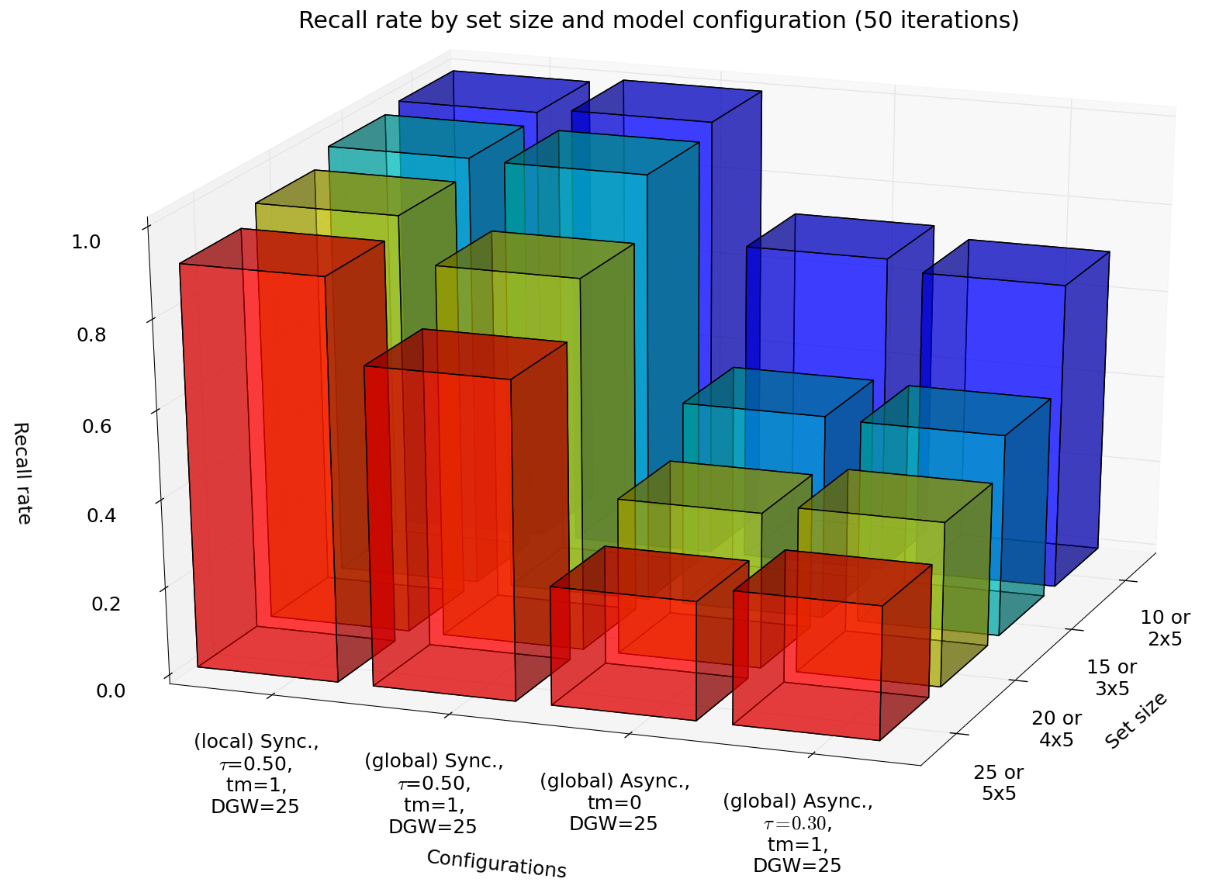
\includegraphics[width=13cm]{fig/i-iters/50-iters-recall}
    \caption{Displaying further recall results for four different model schemes, three of which are global, and one which is local. What distinguishes this plot from the previous are the \textbf{50 training iterations} that are used to train the hippocampal model, for each parametrization and configuration.}
    \label{fig:50-iters-recall}
\end{figure}

\begin{figure}
    \centering
    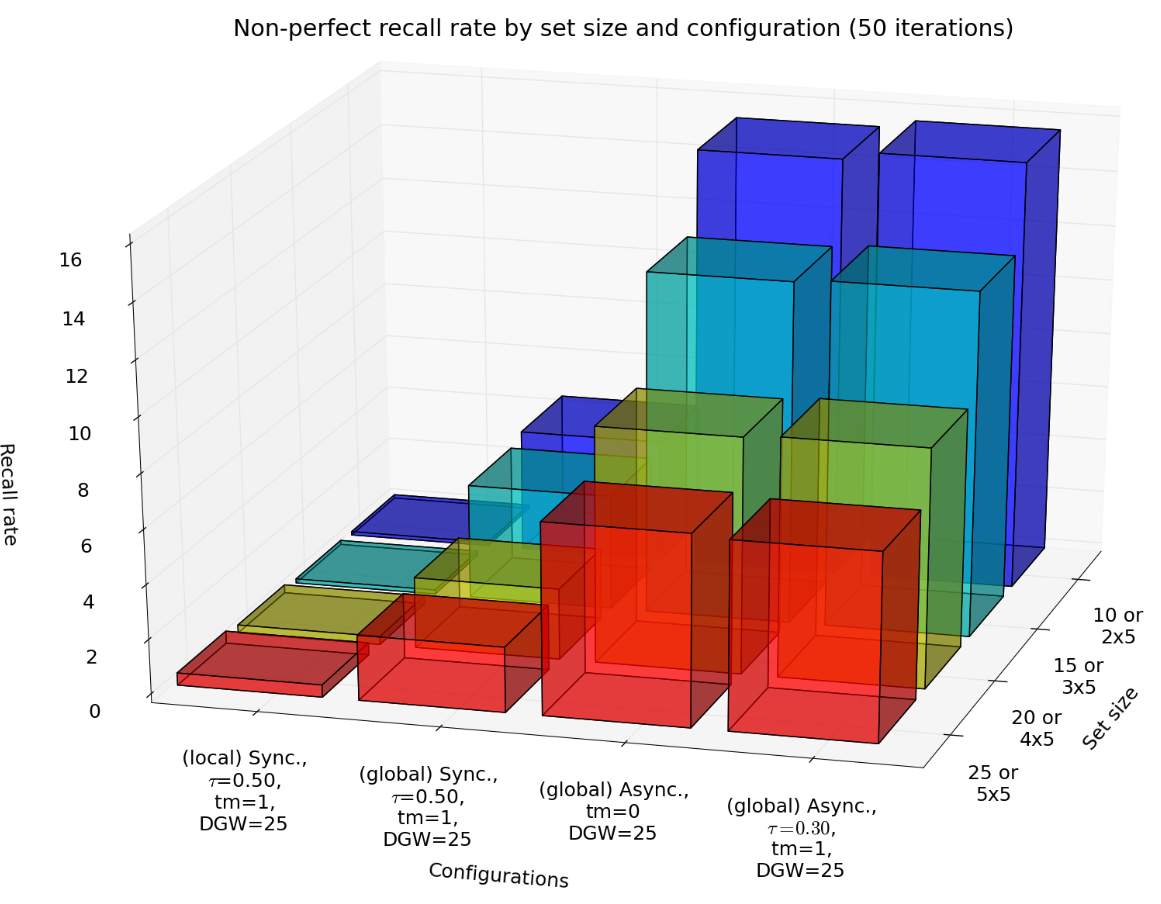
\includegraphics[width=13cm]{fig/i-iters/50-iters-recall-spurious}
    \caption{A 3-dimensional graph of the \textbf{spurious recall rate by set size and model schemem, each model trained for 50 iterations}, corresponding to the perfect recall rates attained and displayed in figure \ref{fig:50-iters-recall}.}
    \label{fig:50-iters-recall-spurious}
\end{figure}

When analysing the spurious recall rate of the asynchronous schemes during chaotic recall, the asynchronous setups are far worse off than the synchronous. Making it apparent that the potentially increased perfect recall rate in the asynchronous schemes in figures \ref{fig:local-recall} and \ref{fig:local-recall-spurious} comes at the cost of drastically increasing the number of spuriously recalled patterns. Conversely and interestingly, spurious recall is still constrained in the synchronous updating mode. This may be due to the fact that asynchronicity simply may introduce more combinations of the previous basins of attraction, whereas the synchronicity greatly constrains the outcome space given the weight configuration. Thus, asynchronous CA3-updating may lead to the output after chaotic recall being a previously unseen, distinct spuriously recalled pattern for every spurious chaotic recall iteration. However, the fact that the synchronous mode is not prone to recalling that many chaotic patterns in the global training exposure scheme mode may may indicate that the model does in fact converge well during training, also in terms of pattern separation. By considering that the perfect recall rate remains very high, but the spurious patterns extracted grows only slightly when increasing the training set size by a factor of 5, indicates that a more complete pattern-completion mechanism may be a central aspect which needs improvement in order to enhance the model performance, and possibly pattern emergent pattern separation ability.

Addressing the success observed by using neuronal turnover for every training set iteration in the synchronous CA3 updating scheme: 
This will necessarily increase the pattern separation capabilities of the model dynamically, as the model by rewiring parts of its connections thus will re-code the presented k-winners pattern to the preceding layer. However, as this is also performed for each exposure to the same pattern, it remains a bit unclear how it still enhances the separation ability. My take on this is that more randomness in re-instantiating the synapses will lead to varying the k-WTA pattern, which again will be consolidated for the successfully separated patterns dynamically, as Hebbian learning wires the neurons that are simultaneously firing, enhancing the connections that are more persistent, and thus highly correlating, more than others. Thus, re-instantiation of synaptic connections, or neuronal turnover, becomes a type of dynamic trial-and-error in pattern separation, which may be successful due to the fact that lateral inhibition is simulated by the k-WTA algorithm, which favours a certain layer-wise stability.

% ================ Hetero-associative training patterns ===============
\subsection{Hetero-associative training patterns}\label{sect:hetero-associative}

In order to verify that the hippocampal model generalises to training sets of hetero-associative training patterns, which after all may be said to generally be the nature of training training data, hippocampal model performance is evaluated using the hetero-associative training patterns illustrated in figure \ref{fig:hetero-associative-patterns}.

\begin{figure}
    \centering
    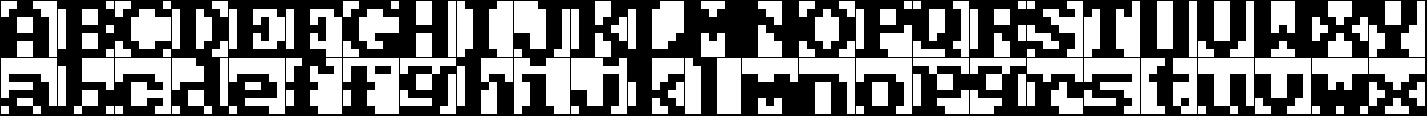
\includegraphics[width=13cm]{fig/im_both_hetero}
    \caption{Displaying \textbf{the hetero-associative training set}, the first row being the pattern inputs, and the second being the associated outputs.}
    \label{fig:hetero-associative-patterns}
\end{figure}

\begin{figure}
    \centering
    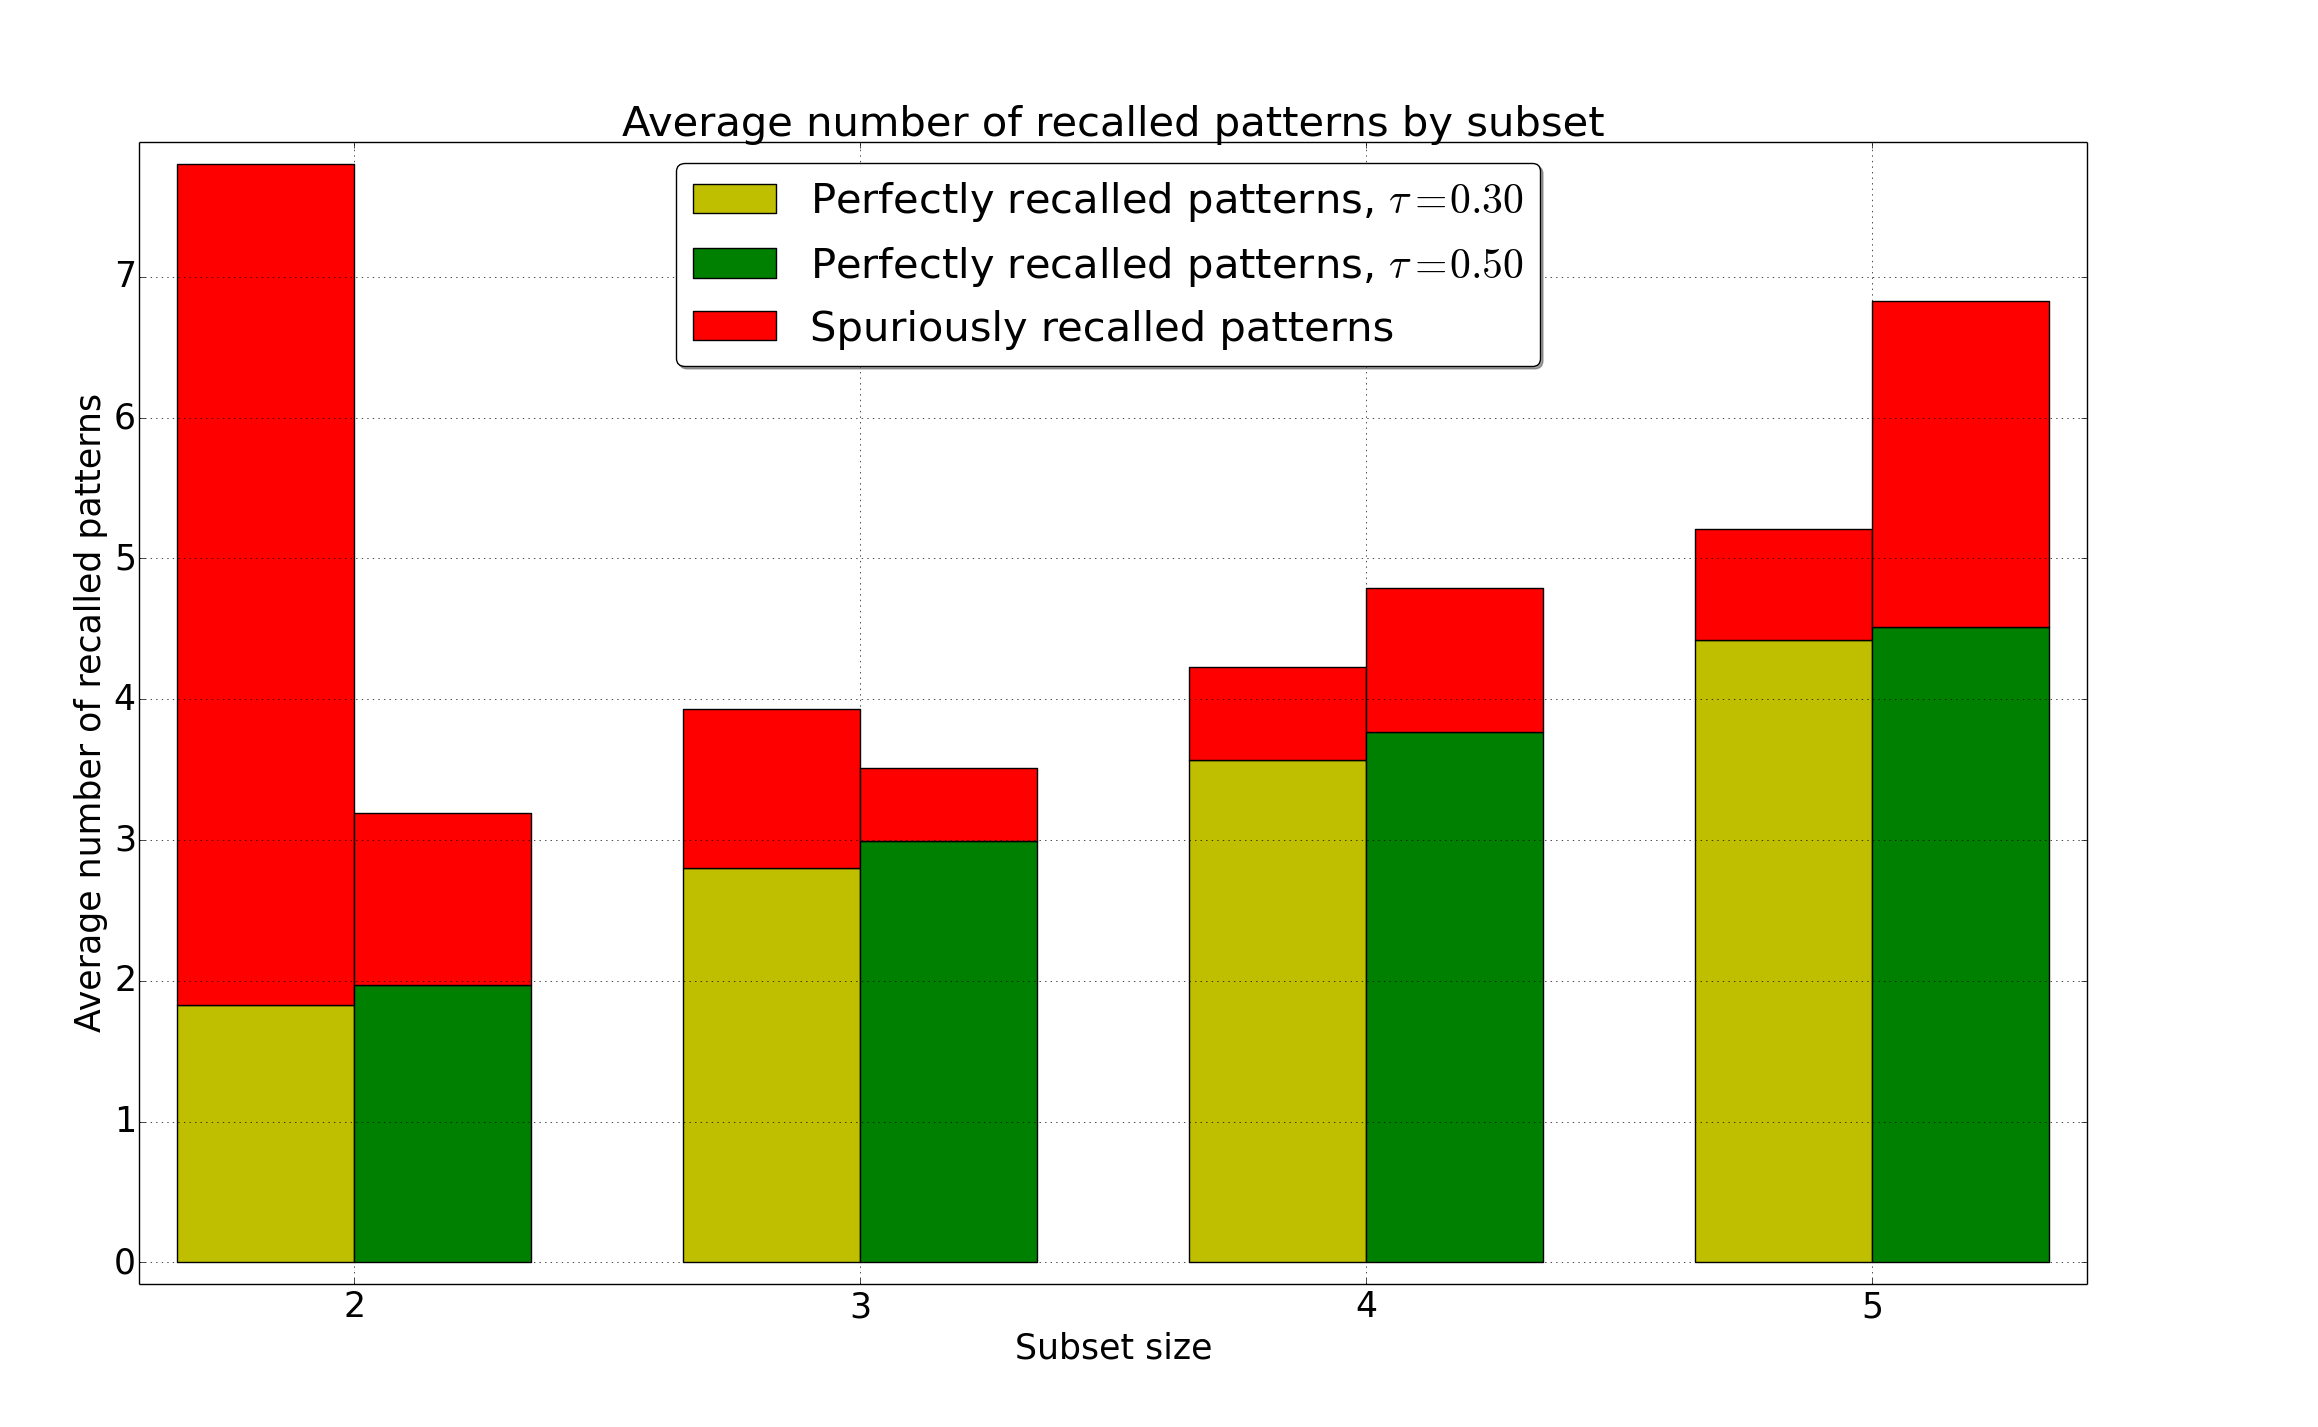
\includegraphics[width=15cm]{fig/tr50_tr30}
    \caption{\textbf{Displaying the number of recalled patterns} when training on the hetero-associative training set, using the two best model configuration schemes attained in this thesis.}
    \label{fig:hetero-results}
\end{figure}

Note that the results in figure \ref{fig:hetero-results} demonstrate a performance of approximately equal quality as in the auto-associative case. Furthermore, when using a turnover rate $\tau$ of $0.30$, the same interesting phenomenon of a very large number of spuriously extracted patterns relatively is observed for set size 2x5. This may indicate that there is some mechanism at play which reflects internal model behaviour, rather than training set specific results for this training set size. What this is remains somewhat obscure. One hypothesis includes that pattern separation might not have had time to occur succinctly before training is regarded as complete. This hypothesis is further strengthened when considering that the increase in $\tau$ significantly decreases the number of spuriously extracted patterns. Furthermore, when the set size grows larger, a turnover of $\tau=0.50$ shows an increase in the number of spurious pattern recall. Note that this also strengthens the view of the trade-off between successful pattern separation and spurious recall. Interestingly, the spuriously recalled patterns also seem to encode the principal correlations of the patterns in the data set, resulting in equal, or in fact enhanced neocortical model performance in terms of the goodness of fit in the previous section \ref{section:hpc-experiments}. Neocortical memory consolidation is not performed here for the hetero-associative training patterns, as this would require expanding the hippocampal model significantly, or designing a permuting input with the extracted chaotic outputs scheme, which would remain fairly biologically unrealistic. Therefore, memory consolidation in the case of hetero-association is considered to be outside the scope of this thesis.

\subsection{Model comparison}

\begin{table}[]
\centering
\caption{Showing the approximate average perfect recall rate values using \textbf{auto-associative} training patterns for the conventional state-of-the-art model of \citep{Hattori2014}, and the novel model implemented in this thesis. See figures \ref{fig:local-recall}, \ref{fig:global-recall}, and \ref{fig:50-iters-recall} for figures illustrating the attained recall rates.}
\label{table:comparison-perfect-recall-rates}
\begin{tabular}{|c|c|c|c|c|}
\hline
\multicolumn{5}{|c|}{Perfect recall rates}                                         \\ \hline
Pattern set size   & 2x5           & 3x5           & 4x5           & 5x5           \\ \hline
Conventional model & 1.00 & 0.98 & 0.91 & 0.81 \\ \hline
Novel model        & 1.00 & 0.98 & \textbf{0.96} & \textbf{0.90}  \\ \hline
\end{tabular}
\end{table}

\begin{table}[]
\centering
\caption{Showing the approximate average perfect recall rate values using \textbf{hetero-associative} training patterns for the best model scheme as displayed in figure \ref{fig:hetero-results}. Comparing the conventional model from \citep{Hattori2014} with the novel implemented model.}
\label{table:comparison-perfect-recall-rates-hetero}
\begin{tabular}{|c|c|c|c|c|}
\hline
\multicolumn{5}{|c|}{Perfect recall rates}                                         \\ \hline
Pattern set size   & 2x5           & 3x5           & 4x5           & 5x5           \\ \hline
Conventional model & 1.00 & 1.00 & \textbf{0.97} & 0.88 \\ \hline
Novel model        & 0.99 & 1.00 & 0.94 & \textbf{0.90}  \\ \hline
\end{tabular}
\end{table}


When comparing the attained model results in tables \ref{table:comparison-perfect-recall-rates} and \ref{table:comparison-perfect-recall-rates-hetero}, the novel model parametrization and CA3-updating scheme appears to be better at pattern separation for auto-associative training patterns, possibly due to its significantly increased neuronal turnover rate. In training on hetero-associative training patterns, the model performance appears to be approximately equal, perhaps slightly better in the conventional model for set size 4x5, having an extraction rate which is $3 \%$ higher than the novel model. However, as particularly evident for auto-associative patterns, the novel model still seems to be better at tackling the largest set size; 5x5, where the extraction rate is $0.02$ more than for the conventional model.

% ======================== summary hpc ===========================
\subsection{Hippocampal module results summary}

Under the less stringent convergence criterion of training or recalling for 15 iterations, it became apparent that the trends for one model configuration demonstrate significantly better performance. Namely the configuration; synchronous updating of the CA3-layer neuronal activation values as well as weight updates, using turnover for every training iteration, a DG-weighting of 25, and a turnover rate of $\tau=0.30$.
This configuration demonstrates a state-of-the-art performance for dual-network memory models in short-term memory pattern extraction and perfect recall rates. Perfect recall rates are significantly better than the models of \citep{Hattori2014, Hattori2010}, with the comparative results are provided in table \ref{table:comparison-perfect-recall-rates}.


To summarise the main findings of the experiments specifically targeting the hippocampal module; the DG-weighting shows no correlation or impact in the asynchronous CA3-updating schemes. However, it seems to be crucial to the performance to set the $DGW=25$ in the synchronous updating modes, which yields about twice the perfect recall rates.

As for the neuronal turnover rate, $\tau$, it seemed to have no effect on neither the perfect recall rate nor the convergence rate using asynchronous CA3-neuronal updating. Furthermore, the average results revealed that there was no clearly visible impact under the synchronous updating scheme when turnover was only being performed between the learnt subsets. However, when turnover is performed for every training iteration, the results demonstrate an increase in hippocampal model performance correlated with an increasing turnover rate - i.e. both the convergence rates and perfect recall rates increased as the turnover rate did up to a certain limit of about 0.3, after which the perfect recall rate increased significantly for set size 3x5, but convergence and perfect recall decreased for set size 5x5, as well as spurious recall rates for all set sizes.

In the last experiment on auto-associative patterns, the relaxed criterion scheme demonstrates that the criteria of having a stable output for three recall iterations when a random input is provided to the network is far too stringent. Furthermore, in the local training set exposure scheme, synchronous CA3-updating, having turnover for every training set iteration, as indicated in the previous experiments on the neuronal turnover rate, is significantly better than the other configurations. It is worth noting also that is displays a rather interesting property for the set size 2x5, i.e. a relatively large number of spuriously recalled patterns. As for the, global training set exposure schemes, synchronous CA3-updating continued to significantly outperform the asynchronous. However, not performing neuronal turnover yielded slightly better model performance in terms of perfect recall. When increasing the number of training iterations to 50, the performance became more even. However, the model behaviour demonstrates a significant advantage of using local subset exposure to the hippocampal and short-term memory model, as this resulted in above $90 \%$ perfect recall rates, along with few spuriously recalled patterns - even fewer when using 50 training iterations. For the best model scheme 50 training iterations deviated very little from when using 15, the main difference being the extraction of less spurious patterns.

Lastly, when training the most successful hippocampal model schemes on the hetero-associative training set, model performance remained fairly equal. This demonstrates a capability of successfully extracting hetero-associative patterns, and furthermore that the emergent model qualities such as pattern separation generalises to heterogeneous data sets. Note that the observed robustness in model performance is in slight contrast to the findings of \citep{Hattori2014}, as his model performance declined slightly when training on auto-associative training patterns, compared to hetero-associative training patterns. This may be due to an increased overlap in pattern-correlations in weight space.




% ================ Neocortical module experiments ===============
\section{Neocortical module experiments}

This section contains the experiments testing the memory consolidation to the neocortical module within the dual-network memory model. Beginning with a fairly short demonstration of convergence and interference in the outlined network with the auto-associative training set, the section is followed by a short section on pseudorehearsal, preceeded by experiments on memory consolidation from the hippocampal module. Note that 'memory' is used throughout this thesis as describing any abstract representation such as a pattern association or functional mapping inherent in the network weight configration, and thus embodied by the network itself, resulting in specific emergent network activity.

Based on the assumption that only successful extraction of patterns in the hippocampal module may provide the basis for successful information transfer to the neocortical module, the best synchronous CA3-updating mode and hippocampal configuration is selected as the model scheme for which neocortical memory consolidation is performed. Furthermore, as I wish to investigate the potential information inherent in spurious patterns, asynchronous updating scheme is also included. Consolidation using chaotically recalled patterns and hippocampal pseudopatterns is also examined in this regard, and to draw potential biological parallels.


% ========================== Subsection =========================
\subsection{Goodness of fit}

In evaluating the performance of the neocortical module, the goodness of fit measure, $g$, is adapted from \citep{Hattori2010, Hattori2014}. It is defined as the following,

\begin{equation}
    g = \frac{1}{N} \sum_{i=1}^{N}o_it_i,
\end{equation}

where $o_i$ is the target output vector for pattern $i$, $N$ is the number of patterns in the current training set, and $t_i$ is the target output vector. Note that as the outputs are bipolar, i.e. 1 or -1, in the case of matching only 50 \% of the output, the goodness of fit will be 0.

Note that the model in being a FFBP ANN is not necessarily able to extract perfect pattern correlations, the goodness of fit measure is well suited for measuring a closeness in perfect correlation - where 1 is perfectly extracted, 0 is 50 \% - i.e. random performance, and -1 is perfectly negatively correlated.
The goodness of fit will therefore be the main measure in evaluating the consolidation quality, as well as the network performance.

% ========================== Subsection =========================
\subsection{Model demonstration and potential catastrophic forgetting}

Before delving into the experiments of the neocortical module, I would like to outline and demonstrate how learning of all pattern associations may be successfully attained in the feed-forward back-propagation (FFBP) network studied in this section. This may be achieved by introducing the training set as a global training set, i.e. training on every single of the say 25 patterns (in the 5x5-case) sequentially for a large number of iterations. This will lead to the successful convergence and a goodness of fit measure $g$ of above 0.99 in most cases. However, when constructing sequentially detached training sets, i.e. 5 subsets of the 25 patterns, allowing the model to train only on one subset at a time, results in catastrophic interference in the model. This brings us to the very core of the dual-network memory architecture; as everything cannot be learnt sequentially as a global training set, at least not biologically speaking, an architecture where subsets may be learnt rapidly by a short-term memory, may allow for the slow consolidation to a long-term memory such that its former memories are not disrupted.

\begin{figure}
    \centering
    
\includegraphics[width=13cm]{fig/neo-intro-demo/global_aggregate_im}
    \caption{Displaying the bipolar, \textbf{recalled output for the neocortical network after training} on all of the associative training patterns sequentially (as one training set) for 15 iterations. The goodness of fit of the network is $g\approx0.99$.}
    \label{fig:global_aggregate_im}
\end{figure}

\begin{figure}
    \centering
    
\includegraphics[width=13cm]{fig/neo-intro-demo/local_aggregate_im}
    \caption{Illustrating \textbf{catastrophic forgetting in the neocortical network}, after it has been trained on each subsets of the associative training patterns sequentially (5x5), each for 15 iterations. Note that the recalled output is the model output after being presented with the corresponding input pattern, presented as bipolar values. The goodness of fit of the network is $g\approx0.79$.}
    \label{fig:local_aggregate_im}
\end{figure}

% ========================== Experiment =========================
\subsection{Experiment: Memory consolidation by chaotically recalled patterns}\label{subsect:rand-in-chaotic-out}

In this experiment, the random inputs and the corresponding chaotically recalled outputs (after recalling for 15 iterations), referred to as chaotic, or chaotically recalled patterns, are used in order to attempt to consolidate the functional pattern mapping to the neocortical network. Furthermore, hippocampal pseudopatterns are also used in order to attempt to consolidate the extracted patterns to the neocortical network, the hippocampal pseudopatterns being defined as outlined in chapter \ref{subsection:hpc-pseudopatterns}, now with the relaxed, constant convergence criterion embedded in their generation processes, defined as,

\begin{enumerate}[I.]
    \item A random pattern is generated and input to the hippocampal network, which with the corresponding output after 15 recall iterations is a pseudopattern type I.
    \item Each element of a chaotically recalled output changes its sign with probability P, here set to $P=0.1$, and the pattern is input to the hippocampal network, which with the corresponding output after 15 recall iterations is a pseudopattern type II.
\end{enumerate}

Note that pseudopatterns type I as described above essentially are chaotically recalled patterns. Thus the analysis of the inclusion of them does in a way only extend the number of chaotically recalled patterns used in the training set, which may potentially alter the performance.

Following are the hippocampal model configurations used for memory consolidation to the neocortical network model, "DGW" denoting the dentate gyrus weight coefficient:

\begin{itemize}
    \item Synchronous CA3-updating, DGW = 25, turnover every training iteration, $\tau=0.30$, using 15 training iterations in the hippocampal model.
    \item Synchronous CA3-updating, DGW = 25, turnover every training iteration, $\tau=0.30$, using 50 training iterations in the hippocampal model.
    \item Asynchronous CA3-updating, DGW = 1, turnover between every learnt subset, $\tau=0.50$.
    \item Asynchronous CA3-updating, DGW = 25, turnover for every training iteration, $\tau=0.30$.
\end{itemize}

\begin{figure}
    \centering
    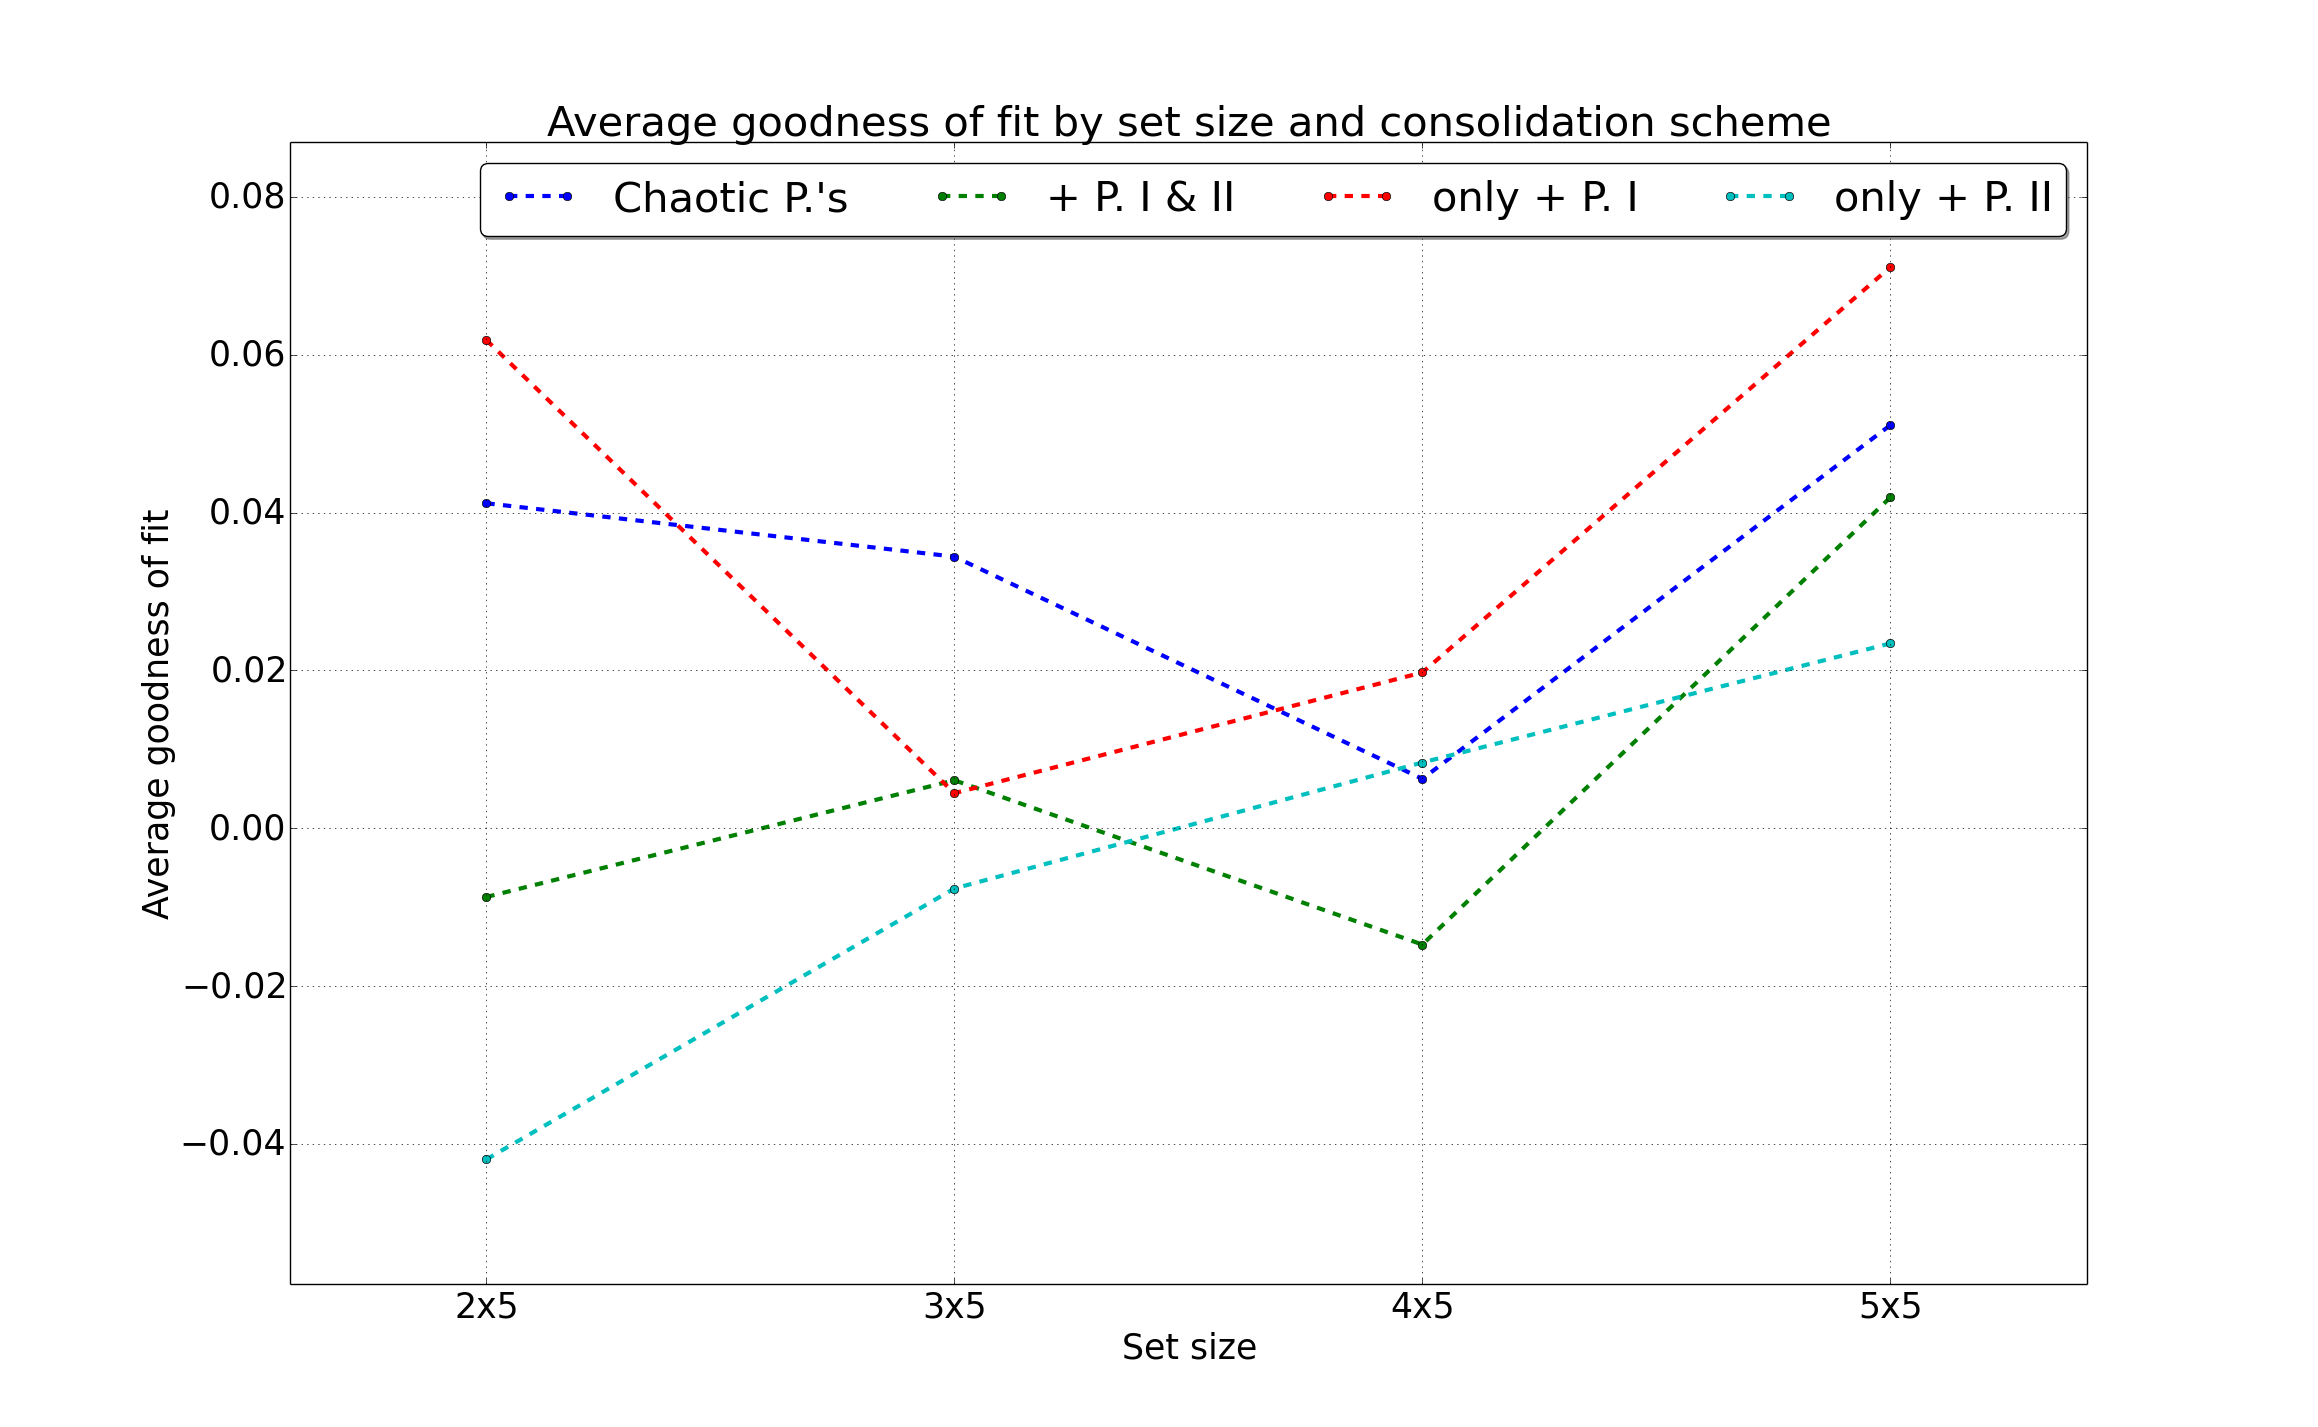
\includegraphics[width=14cm]{fig/neo-consolidation/consolidation-schemes-sync-tm1-tr30_15_iters}
    \caption{Displaying the average goodness of fit for four different consolidation schemes when training for 15 iterations per subset, namely; \textbf{(1)} by only using the chaotically recalled patterns as the training patterns, \textbf{(2)} by using the chaotically recalled as well as pseudopatterns I and II, \textbf{(3)} by using the chaotically recalled patterns and pseudopatterns type I, and \textbf{(4)} by using chaotically recalled patterns and pseudopatterns II. Here the first hippocampal model configuration as listed above is the one which is used, namely synchronous CA3-updating, DGW = 25, turnover for every training iteration, $\tau=0.30$, and training for 15 iterations per subset. Note that the average goodness of fit seems to be approximately 0 in all consolidation schemes.}
    \label{fig:consolidation-schemes-sync}
\end{figure}

The results displayed in figure \ref{fig:consolidation-schemes-sync} suggest that no information is transferred by using any combination of chaotically recalled hippocampal patterns for the hippocampal recall scheme, as the goodness of fit remains approximately 0 for including pseudopatterns I, II, or both I and II. Furthermore, when halving the pseudopattern set size, or if increasing the number of training iterations per subset to $200$, the performance remains the same; $g\approx 0$. Lastly, the consolidation performance, i.e. average goodness of fit, remains approximately $0$ in all of the hippocampal model schemes listed above, figures being included in appendix D. 
This raises the question of whether the chaotically recalled patterns contain any qualities which may reduce catastrophic interference, or any information which may suggest biological parallels, and is addressed in the following experiment.

% ========================== Experiment =========================
\subsection{Experiment: A novel memory consolidation scheme} % algorithm/scheme

Due to the fact that the chaotically recalled patterns for a random input, and an attained fairly stable output, consolidated no information to the neocortical network, I here investigate the consolidation performance when using the chaotically extracted output as both input and output to the neocortical network. When only extracting the target outputs for the training set, this would correspond to training on each subset of the original training patterns sequentially for the auto-associative training patterns. This means that a baseline measure is that of the average goodness of fit when training the network on these original subsets, which results in an average goodness of fit $g \approx 0.79$ (see figure \ref{fig:local_aggregate_im} for the results from one of the runs). Furthermore, the baseline averages, i.e. average goodness of fit when training the neocortical network on the original training subsets, are included per subset in the composite model scheme figures. That is, when investigating the performance of using the chaotically recalled output as both input and output for the auto-associative training sets, i.e. essentially relaying the activity of the input and output layers of the hippocampal module.
I would like to point out that biologically speaking, the activity of CA3 is relayed to CA1 in the hippocampus, which is also relayed back to the EC. Although having a take at how this occurs is outside the scope of this thesis, the existence of such pathways may provide a mechanism for relaying heterogeneous patterns to parts of the cortex, such that the input and output of the neural network may correspond roughly to the pattern by relaying the activity of the EC and CA1.

In these experiments, the same four local schemes are used as in the previous experiment, being outlined in section \ref{subsect:rand-in-chaotic-out} above. Each average value is the average over 20 trials for the corresponding model configuration and set size.

% results

\begin{figure}
    \centering
    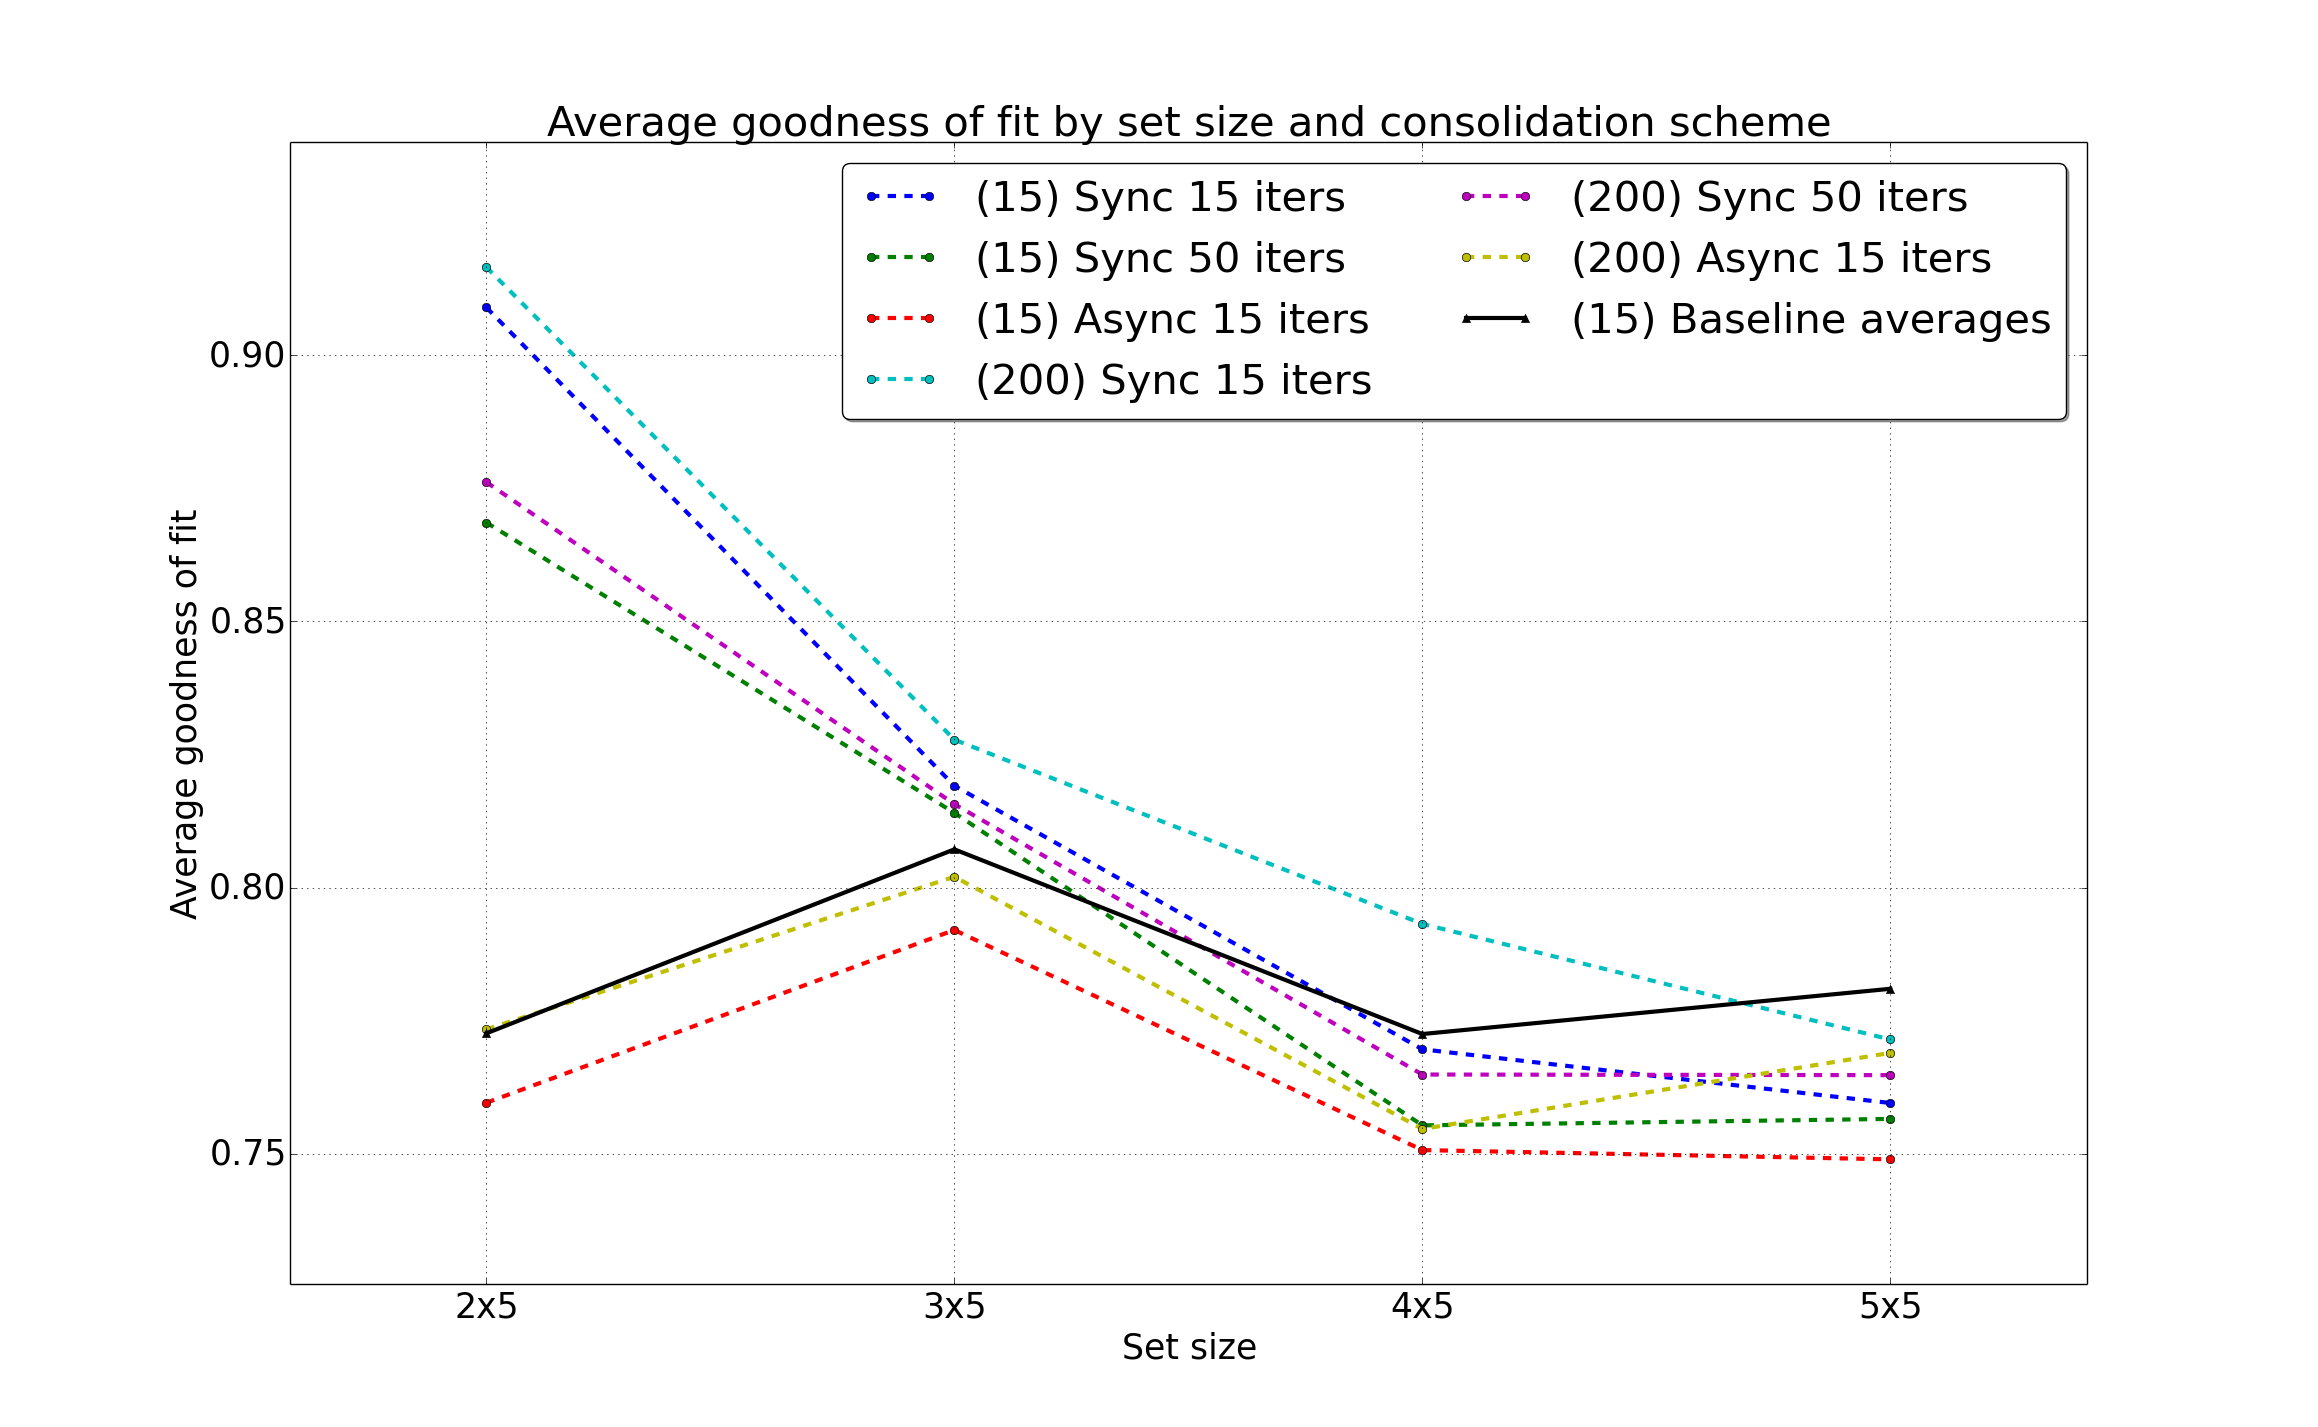
\includegraphics[width=14cm]{fig/neo-consolidation/consolidation-IO-span-all-with-baseline}
    \caption{Illustrating the \textbf{average goodnesses of fit for four different hippocampal model schemes}, all \textbf{using the relaxed training and convergence criterion ($i=15$)} in the hippocampal module. Note that the \textbf{bracketed numbers denote the number of training iterations used in the neocortical network} during pattern consolidation, being either $15$ or $200$, and the thick, \textbf{black line denotes the baseline averages for sequential training on the subsets of the original training set}. It seems that the averages do not deviate significantly from one another, with the exception being for set size 2x5 in the synchronous CA3 updating scheme, where the goodness of fit is significantly improved by using the chaotically recalled patterns as the spanning input and output of the neocortical network.}
    \label{fig:consolidation-IO-span-all-with-baseline}
\end{figure}

It is interesting to note that when distorting the original training patterns, the neocortical network is very sensitive to the number of training iterations used per subset.
However, when using chaotically recalled patterns, it seems that the model is far more robust. This may suggest that the principal correlations are inherent in most chaotically recalled patterns. 
Furthermore, as the hippocampal model performs pattern separation, it may output patterns which are more separated in weight space, and thus more well suited for sequential consolidation to a neocortical network. This may lower the need for pseudorehearsal in order to maintain previous patterns, and is therefore a more biologically realistic mechanism for pattern consolidation. 

\begin{figure}
    \centering
    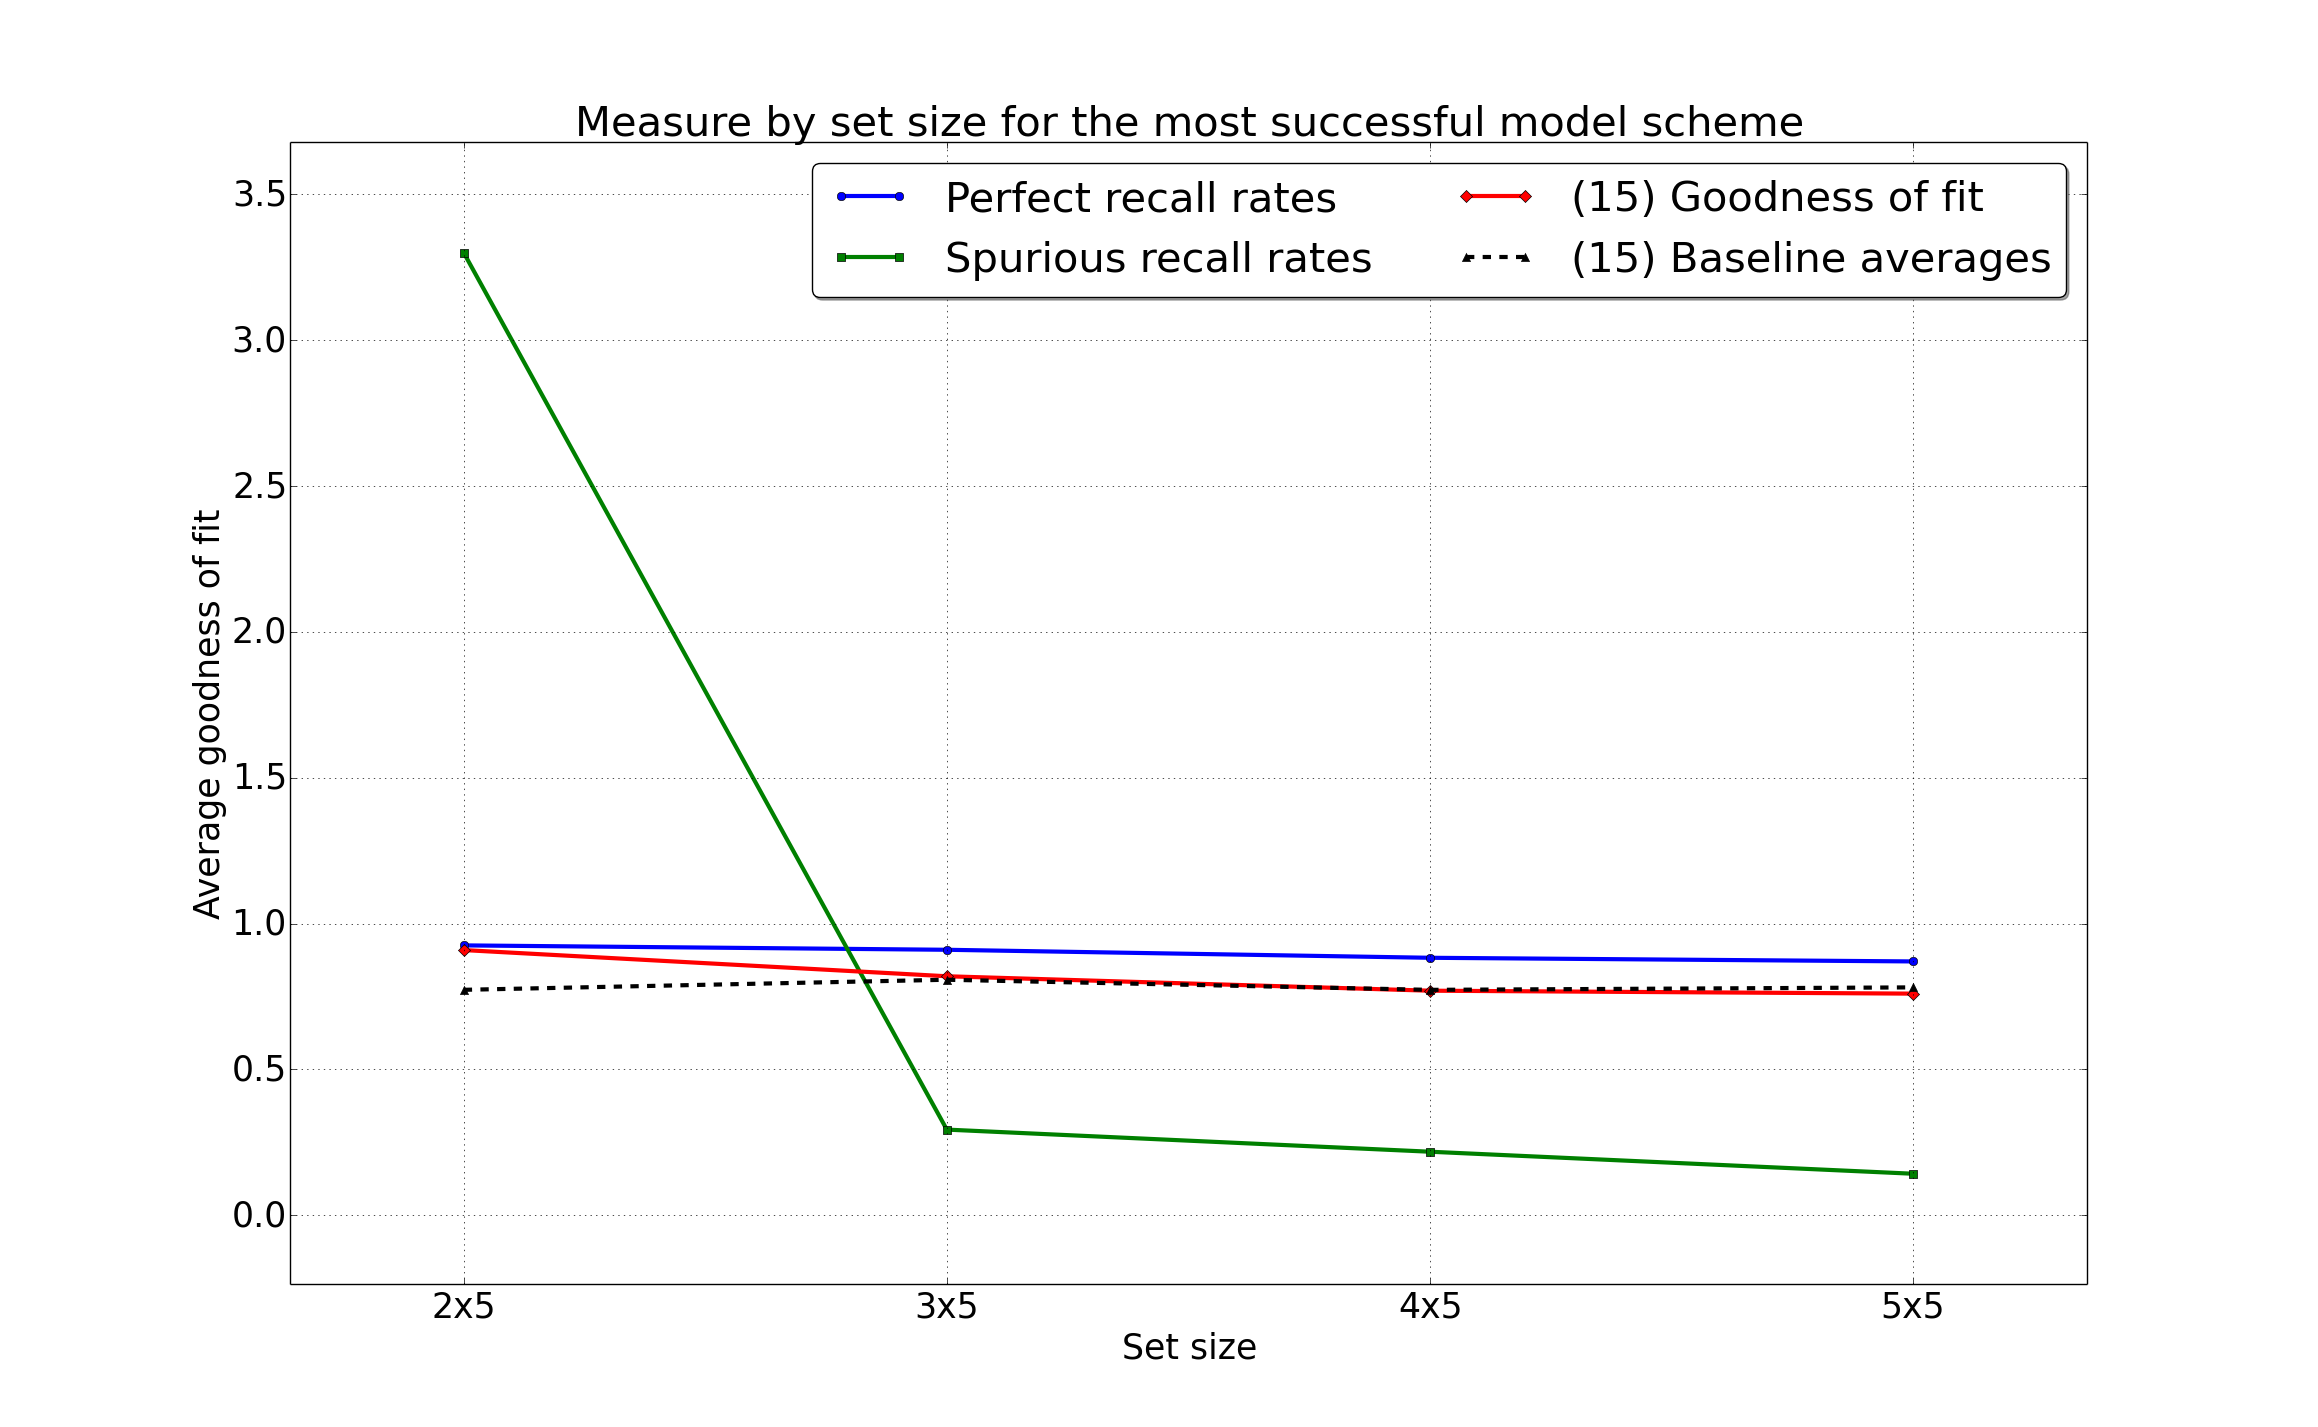
\includegraphics[width=14cm]{fig/neo-consolidation/combined-measures-sync}
    \caption{A plot of the \textbf{main measures used in this thesis to evaluate the dual-network memory model}, using one of the most successfull dual-network memory model schemes attained in this thesis; \textbf{synchronous CA3-updating, $\tau=0.30$, tm$=1$, DGW$=25$, and training on all extracted patterns, using the output as IO to the neocortical network} (i.e. symbolising a potential pathway relaying of the pattern signals). Note that the goodness of fit is approximately the same as the perfect recall rate for set size 2x5, when the relative spurious recall rate is more than 3 times the set size. However, when the set size increases, and the spurious recall rate drops below 0.5, the goodness of fit drops by 0.10. It continues to drop slightly for the preceding set sizes, while starting to flatten out, too. Note that the exact same description fits for the spurious recall rate.}
    \label{fig:combined-measures-sync}
\end{figure}

\begin{figure}
    \centering
    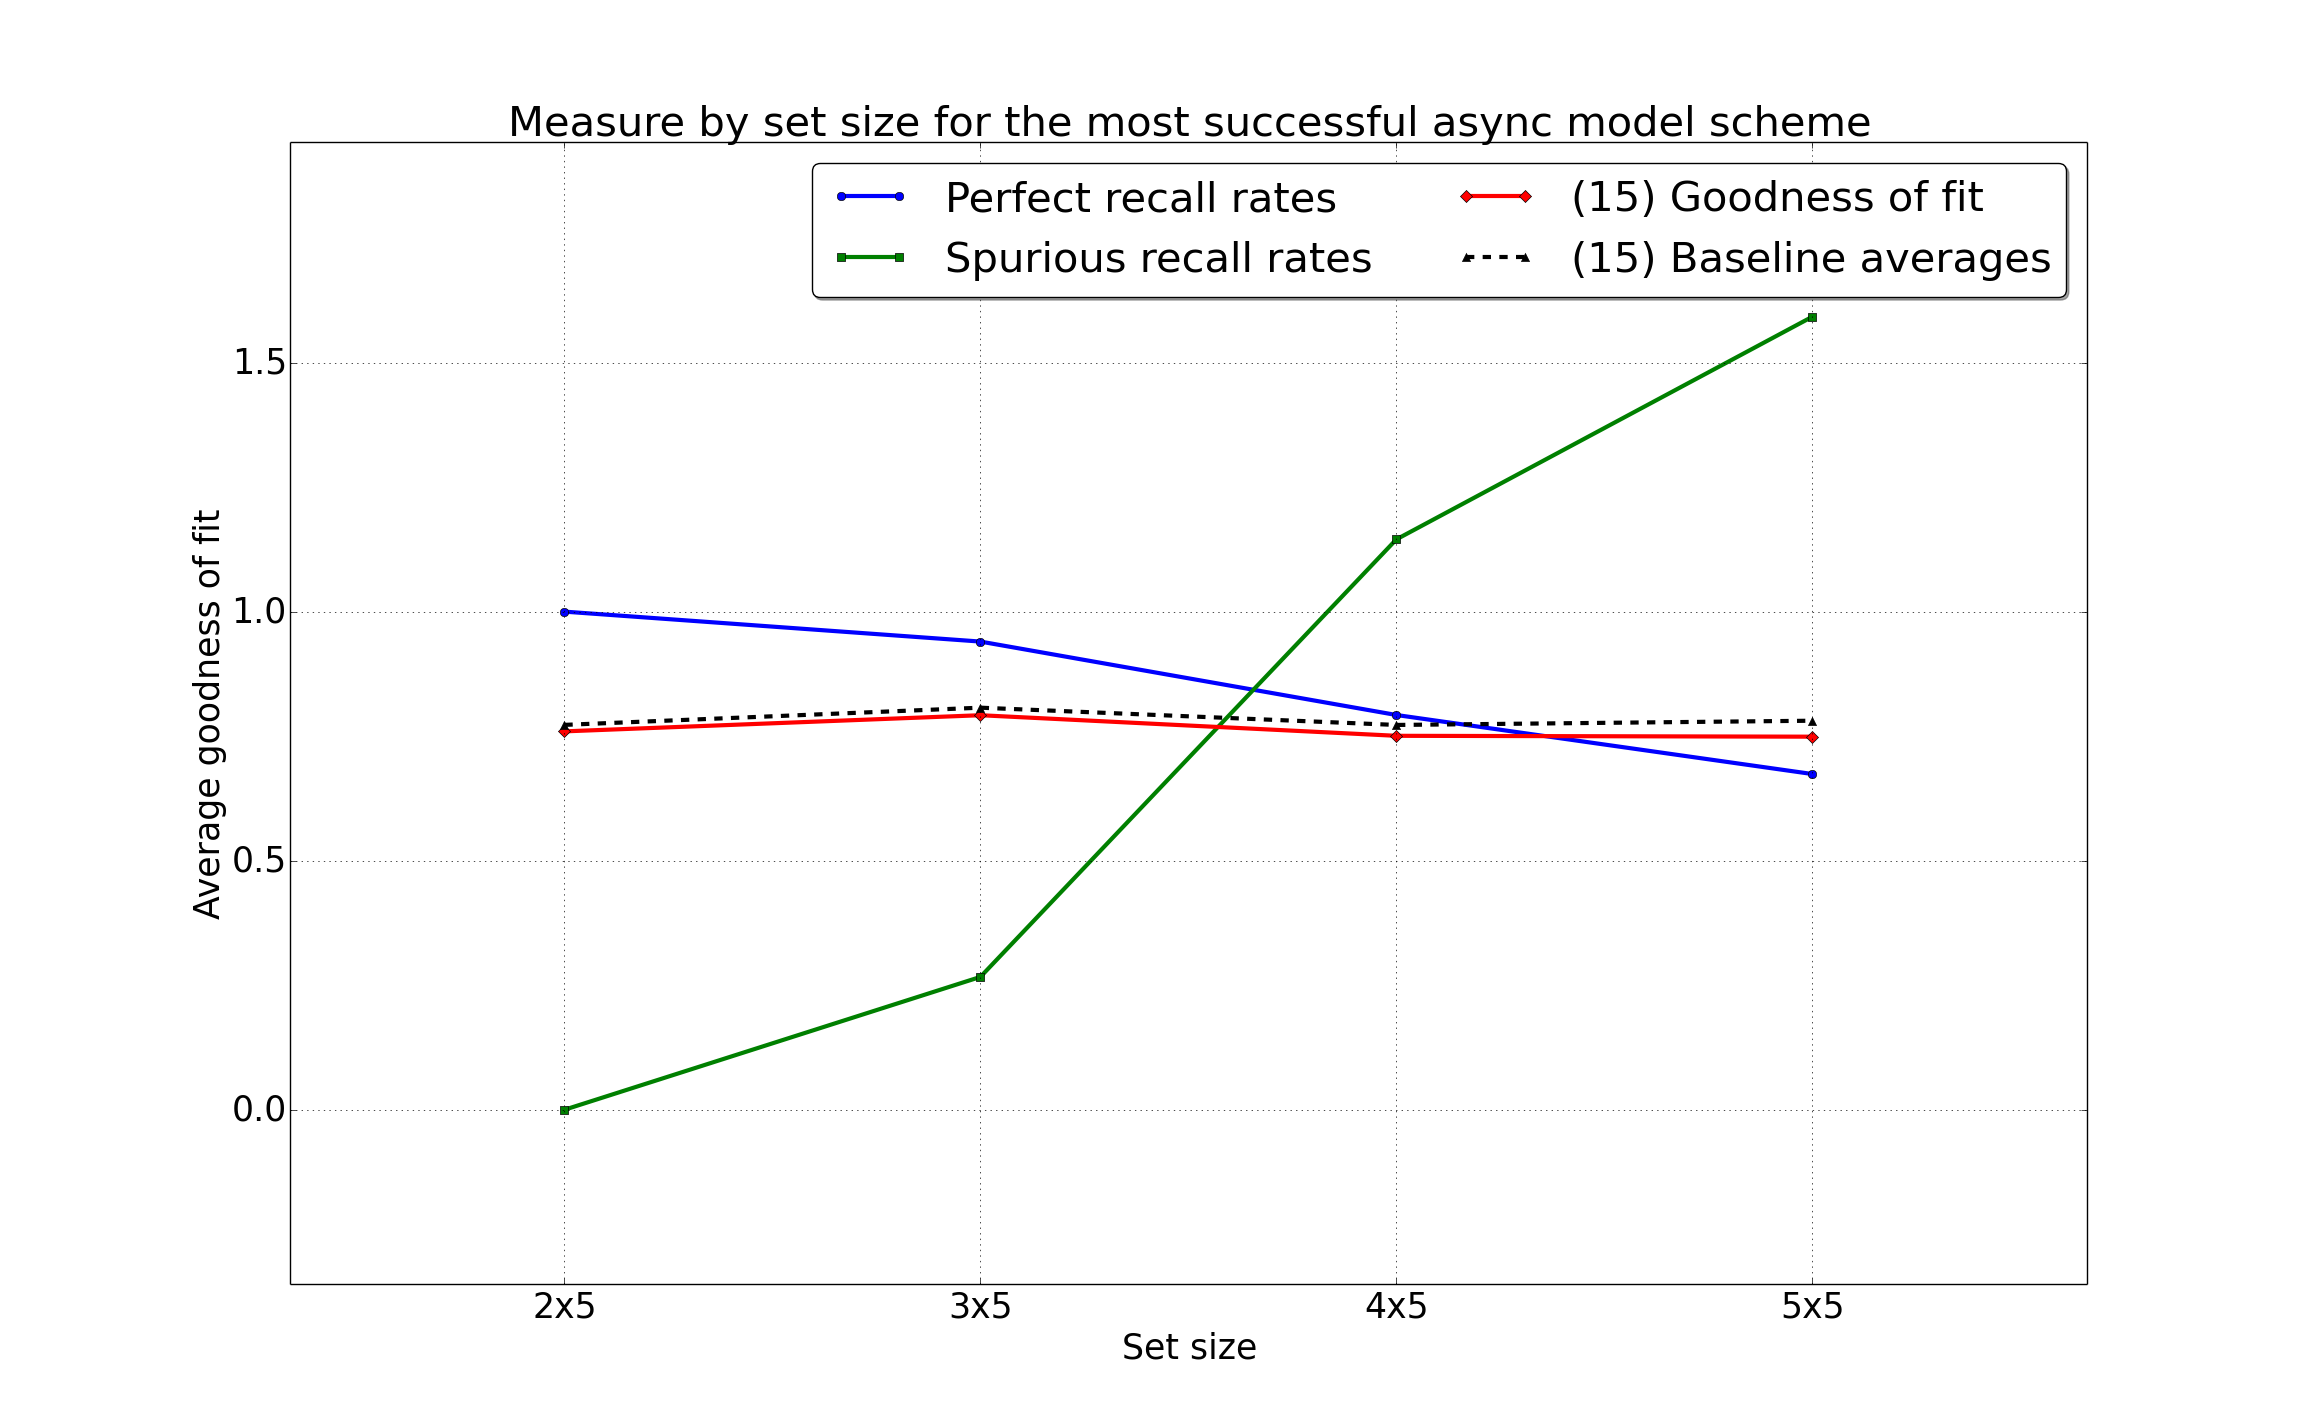
\includegraphics[width=14cm]{fig/neo-consolidation/combined-measures-async}
    \caption{Displaying the \textbf{main thesis measures}, here under the same scheme as in figure \ref{fig:combined-measures-sync}, however, by employing \textbf{asynchronous CA3-updating}. Note that the spurious recall rate seems correlated with a decrease in the perfect recall rate here, as opposed to in the figure for the synchronous scheme.}
    \label{fig:combined-measures-async}
\end{figure}

Note that there seems to be a possible correlation between spuriously recalled patterns and the goodness of fit, when investigating figure \ref{fig:combined-measures-sync}. Furthermore, when investigating figure \ref{fig:combined-measures-async}, it seems that no correlation is present between the two variables - only a negative correlation between the spurious recall rate and the perfect recall rate. Looking back to previous figures in the more stringent convergence scheme, this may reflect the fact that the model when using asynchronous CA3-updating introduces more randomness, and so introduces more truly spurious patterns when failing to convergence. Quite differently, the spurious patterns in the synchronous CA3-updating scheme are present in the mode which is most likely to converge. This might possibly be because the model is allowed to extract patterns by chaotic recall for a larger number of iterations relative to the learnt patterns. 
It is nevertheless a noteworthy observation, that these seem to enable the neocortical network to attain, on average, a high goodness of fit. In fact, this goodness of fit remains approximately the same when varying the training iterations per subset of chaotically recalled patterns in the neocortical network from 15 to 200. This is yet another interesting quality of the chaotically recalled patterns. When training on the subsets of the original training patterns, the average goodness of fit is very insensitive to the number of neocortical training iterations  (see among others figures \ref{fig:combined-measures-sync}, \ref{fig:combined-measures-async}, \ref{fig:consolidation-IO-span-all-with-baseline}). However, the goodness of fit is approximately the same for all set sizes, being approximately $g\approx 0.8$. Furthermore, it does not necessarily follow that this robustness to the number of neocortical training iterations will arise for the goodness of fit, strengthening the view that there may be some biologically realistic mechanisms at play in the creation of spurious chaotically recalled patterns in the best model scheme, particularly for set size 2x5. The same holds when increasing the number of training patterns in the original training set. To see this, it may be demonstrated that the average goodness of fit, if creating a number of very lightly permuted patterns of the original training patterns, falls rapidly. Furthermore, it is highly sensitive to the number of neocortical training iterations. This strengthens the hypothesis that the spurious patterns reflect the principal correlations of the original training set, and further possibly contain information about the separating hyperplanes in weight space generated by the recoding capabilities of the CA3-layer (keep in mind that the hippocampal model is not a FFBP ANN, so it has not been shown that it performs PCA). In order to illuminate the discussion above, a figure of the aggregate neocortical output for the original input patterns is shown in figure \ref{fig:sync-neo-aggregate-output-2x5}.

\begin{figure}
    \centering
    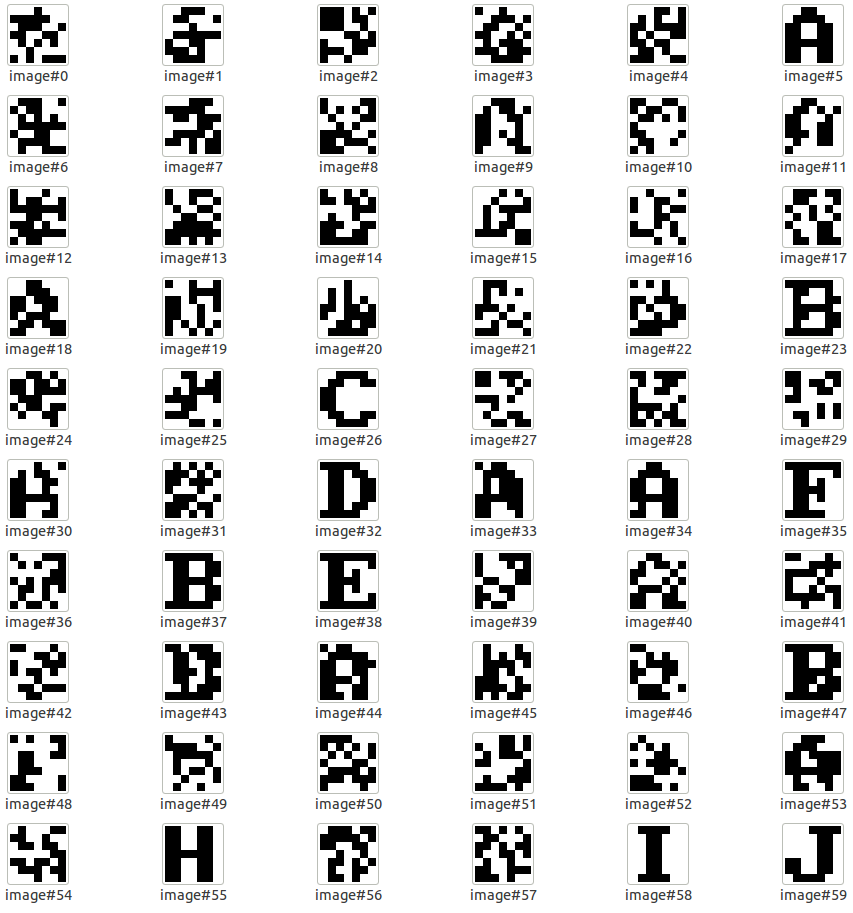
\includegraphics[width=13cm]{fig/neo-consolidation/chaotic-recall-2x5-15-iters-exp0}
    \caption{Displaying the \textbf{patterns extracted by chaotic recall for one single experiment where the dual-network memory model is trained on the 2x5 auto-associative training set}. Note that most of the patterns are non-perfectly recalled patterns, or spurious patterns.}
    \label{fig:chaotic-recall-2x5-15-iters-exp0}
\end{figure}

\begin{figure}
    \centering
    
\includegraphics[width=11cm]{fig/neo-consolidation/one-2x5-run-sync-15-iters42-exp0-15-iters}
    \caption{Illustrating the bipolar \textbf{output of the neocortical network, using the original pattern inputs, after training solely on the chaotically recalled patterns of a single experiment}. Note that the chaotically extracted patterns are displayed in figure \ref{fig:chaotic-recall-2x5-15-iters-exp0}. Note that the original pattern outputs are fairly maintained, and not only the principal elements, resulting in high readability, as opposed to in figure \ref{fig:catastrophic-forgetting-2x5-neo-consolidation}.}
    \label{fig:sync-neo-aggregate-output-2x5}
\end{figure}

Figures \ref{fig:sync-neo-aggregate-output-2x5} and \ref{fig:chaotic-recall-2x5-15-iters-exp0} suggest that the spurious patterns are an aggregate representation of the original training set. By comparison, the neocortical network output when training with catastrophic forgetting on the undistorted original training patterns does not output letters resembling the output patterns for any other than the last two training sets (figure \ref{fig:catastrophic-forgetting-2x5-neo-consolidation}).

\begin{figure}
    \centering
    
\includegraphics[width=11cm]{fig/neo-consolidation/traditional-with-catastrophic-15-neo-iters}
    \caption{Displaying the \textbf{recalled output of the neocortical network after training on the original associative training pattern subsets}, $15$ iterations per subset. Note that the first $3$ out of $5$ subset outputs are completely distorted, and do not resemble the desired output at all.}
    \label{fig:catastrophic-forgetting-2x5-neo-consolidation}
\end{figure}

% last two
\begin{figure}
    \centering
    
\includegraphics[width=11cm]{fig/neo-consolidation/one-2x5-run-sync-50-iters-15-neo-iters}
    \caption{Displaying the \textbf{output of the neocortical network for the inputs of the 2x5 auto-associative training patterns} after training for $15$ iterations on the chaotically recalled patterns in the case of the same model scheme as in figure \ref{fig:chaotic-recall-2x5-15-iters-exp0} - however, here the \textbf{hippocampal model convergence criterion was set to $50$ iterations during training}. It is worth emphasizing that the number of spurious patterns extracted by chaotic recall is $9$, as opposed to in the former case, where it is $51$ (chaotic patterns not displayed).}
    \label{fig:one-2x5-run-sync-50-iters-15-neo-iters}
\end{figure}

\begin{figure}
    \centering
    
\includegraphics[width=11cm]{fig/neo-consolidation/one-2x5-run-async-tm1-15-iters-15-neo-iters}
    \caption{Displaying the \textbf{output of the neocortical network for the 2x5 auto-associative input patterns after training on the chaotically recalled patterns by the hippocampal model when \textit{asynchronous} CA3-updating is used}. Note that $0$ spurious patterns were recalled in this scheme, and that the pattern output of the neocortical recall seems to be erroneous for the two first subsets.}
    \label{fig:one-2x5-run-async-tm1-15-iters-15-neo-iters}
\end{figure}

% \subsection{Distorted IOs demo. - lossless using subset sequential training as baseline measure, but highly sensitive to number of training patterns, i.e. pseudopatterns}

In order to test the hypothesis about the qualities of patterns extracted by chaotic recall and spurious patterns containing crucial information, the scheme of synchronous CA3-updating, with DGW=25, tm=1, and $\tau=0.50$ is also used to generate results which are compared with those of when using $\tau=0.30$, as these model schemes result in slightly different patterns spuriously recalled patterns (see figure \ref{fig:local-recall}). Furthermore, perfect recall and spurious pattern generation is also shown for a novel scheme which is introduced, namely; using $\tau=0.30$, tm=1, DGW=25 in the synchronous updating mode, but having the number of training iterations vary with the set size by a factor of 1.5.

% \begin{figure}
%     \centering
%     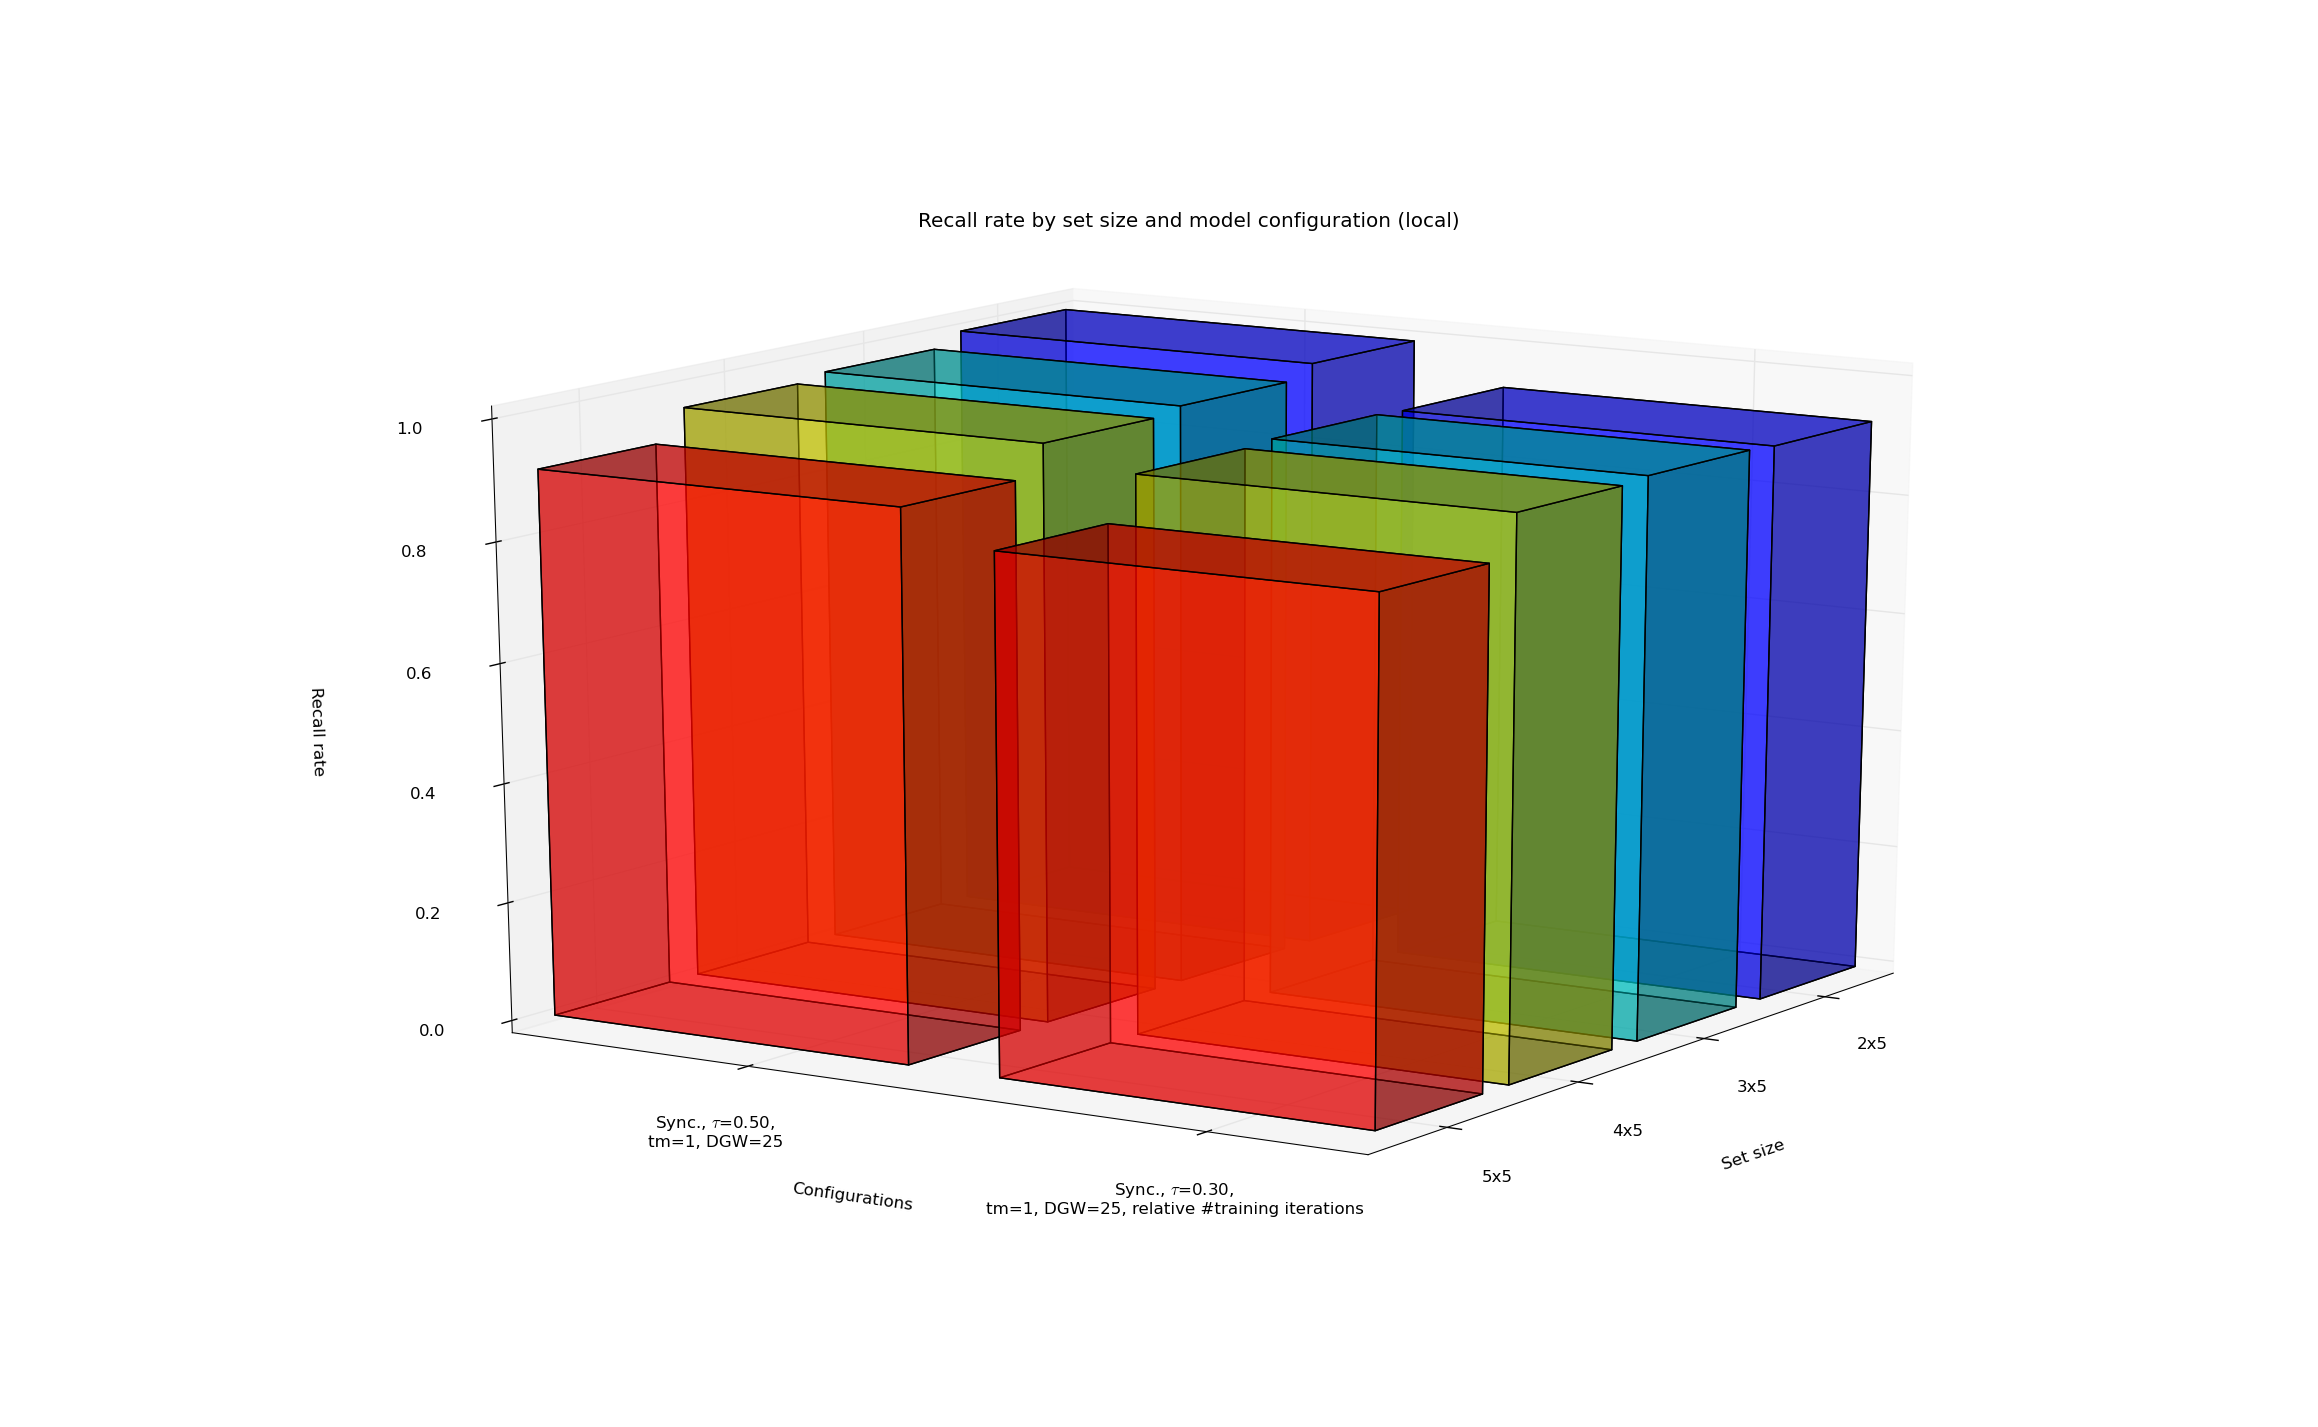
\includegraphics[width=13cm]{fig/hypothesis-test-sync/sync_tests-recall}
%     \caption{the two proposed sync schemes, perfect recall}
%     \label{fig:sync_tests-recall}
% \end{figure}

% \begin{figure}
%     \centering
%     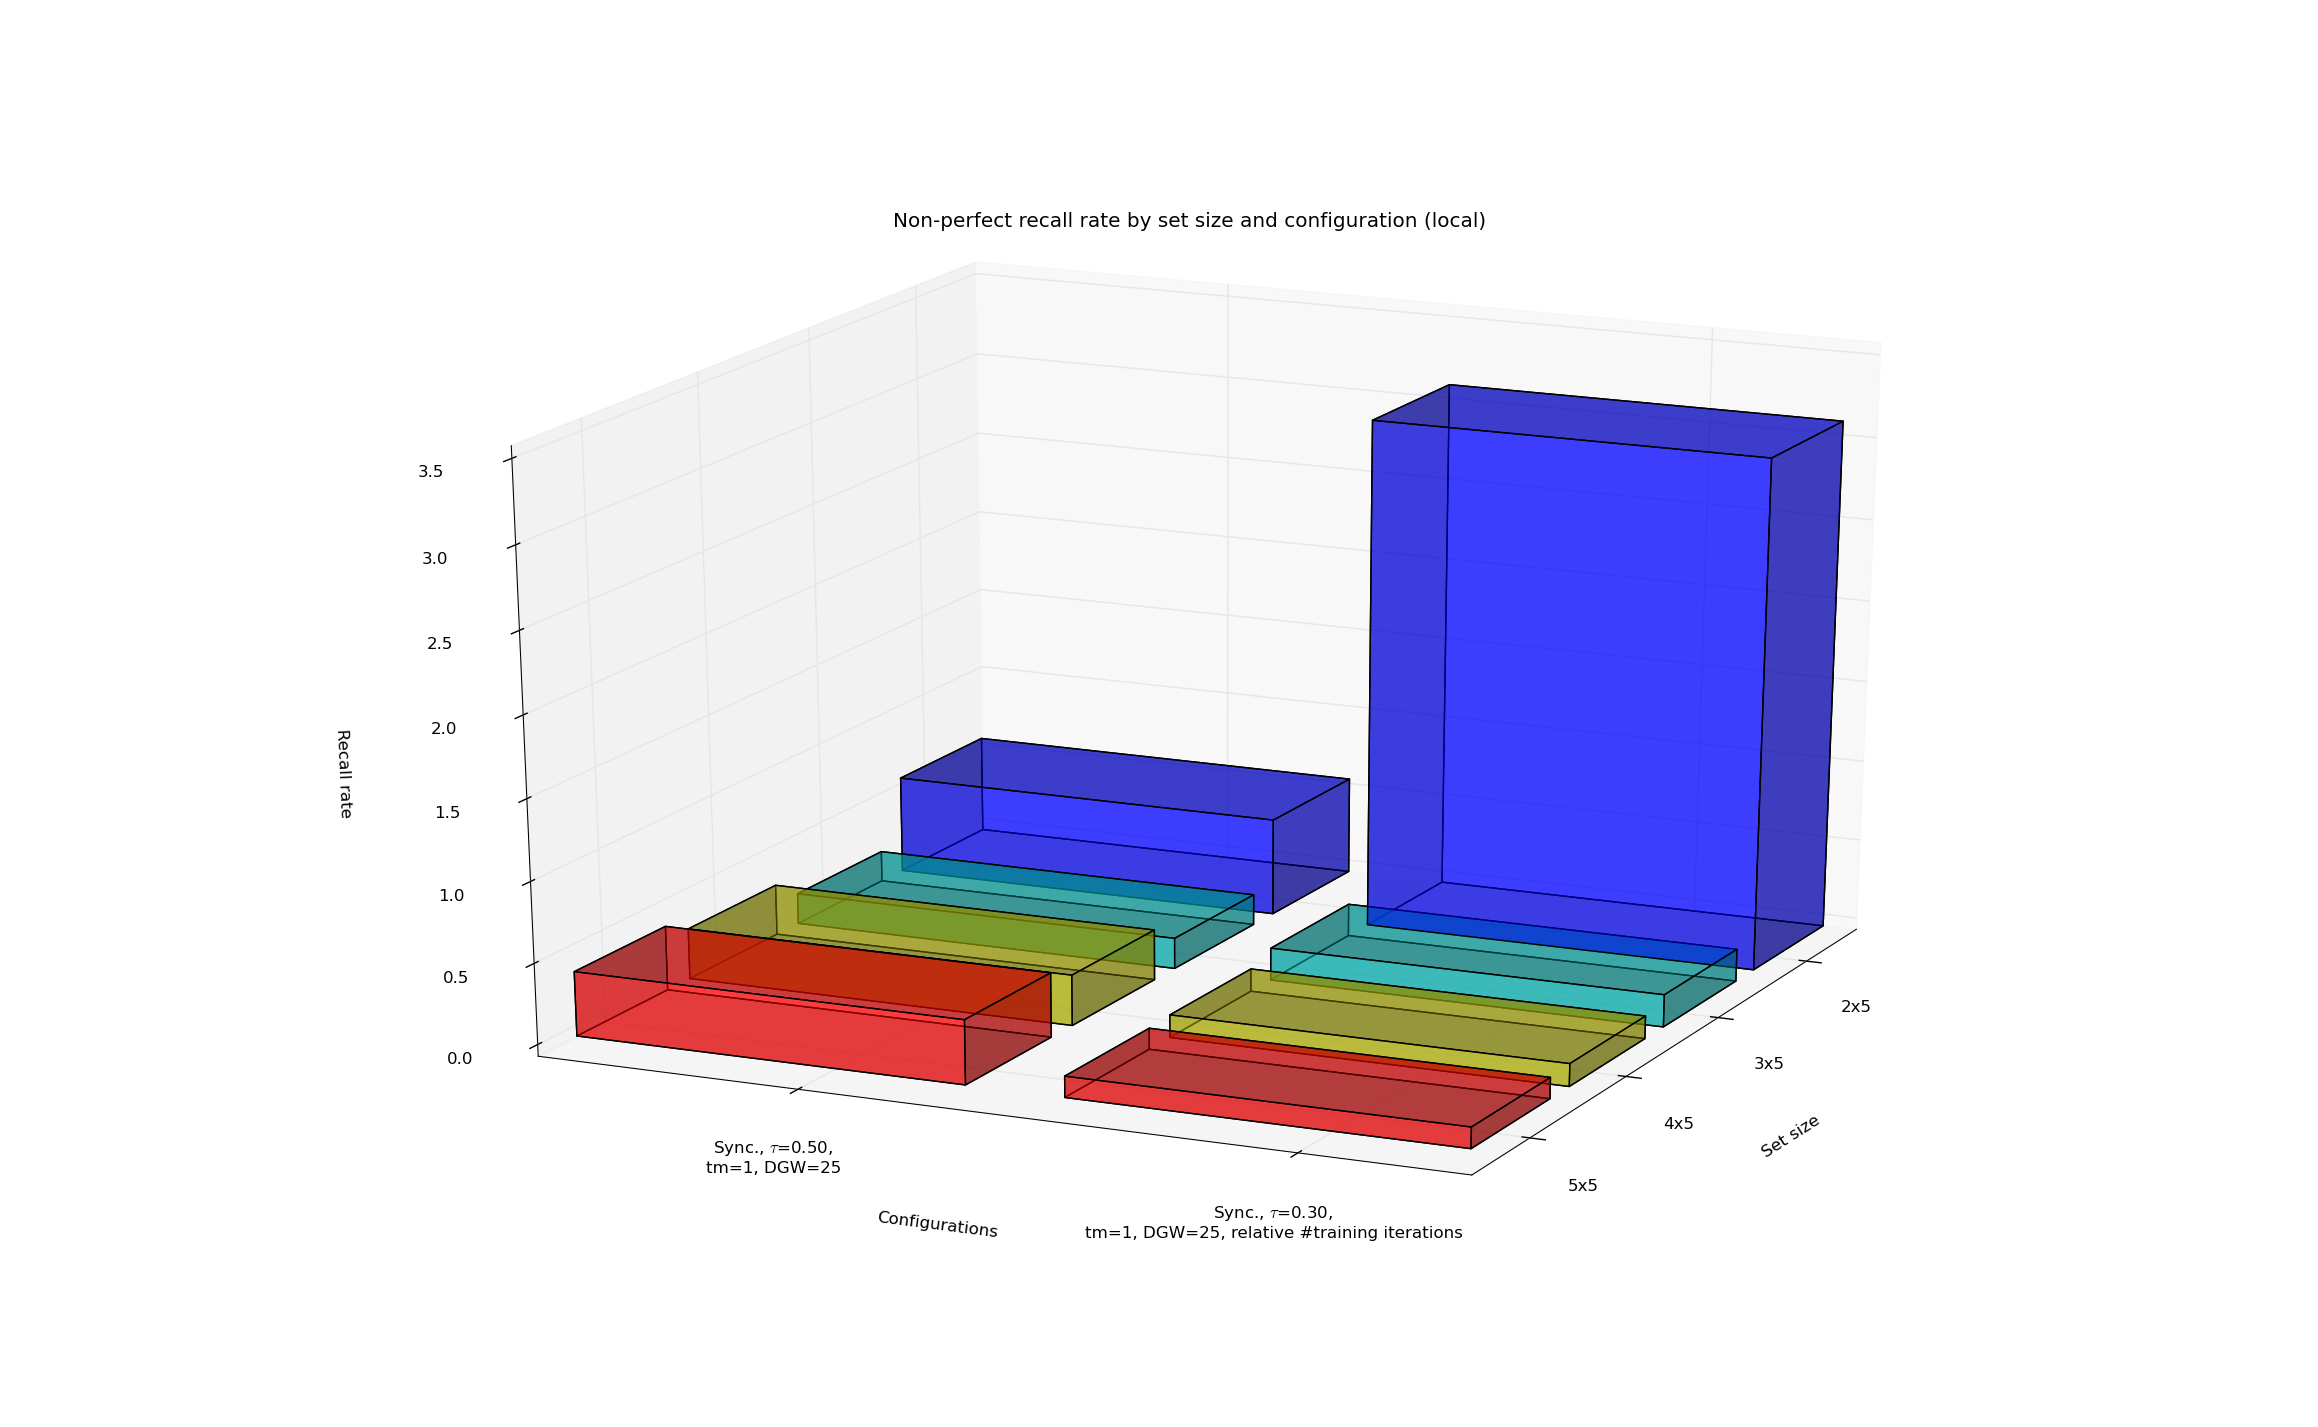
\includegraphics[width=13cm]{fig/hypothesis-test-sync/sync_tests-spurious}
%     \caption{the two proposed sync schemes, spurious recall}
%     \label{fig:sync_tests-spurious}
% \end{figure}

\begin{figure}
    \centering
    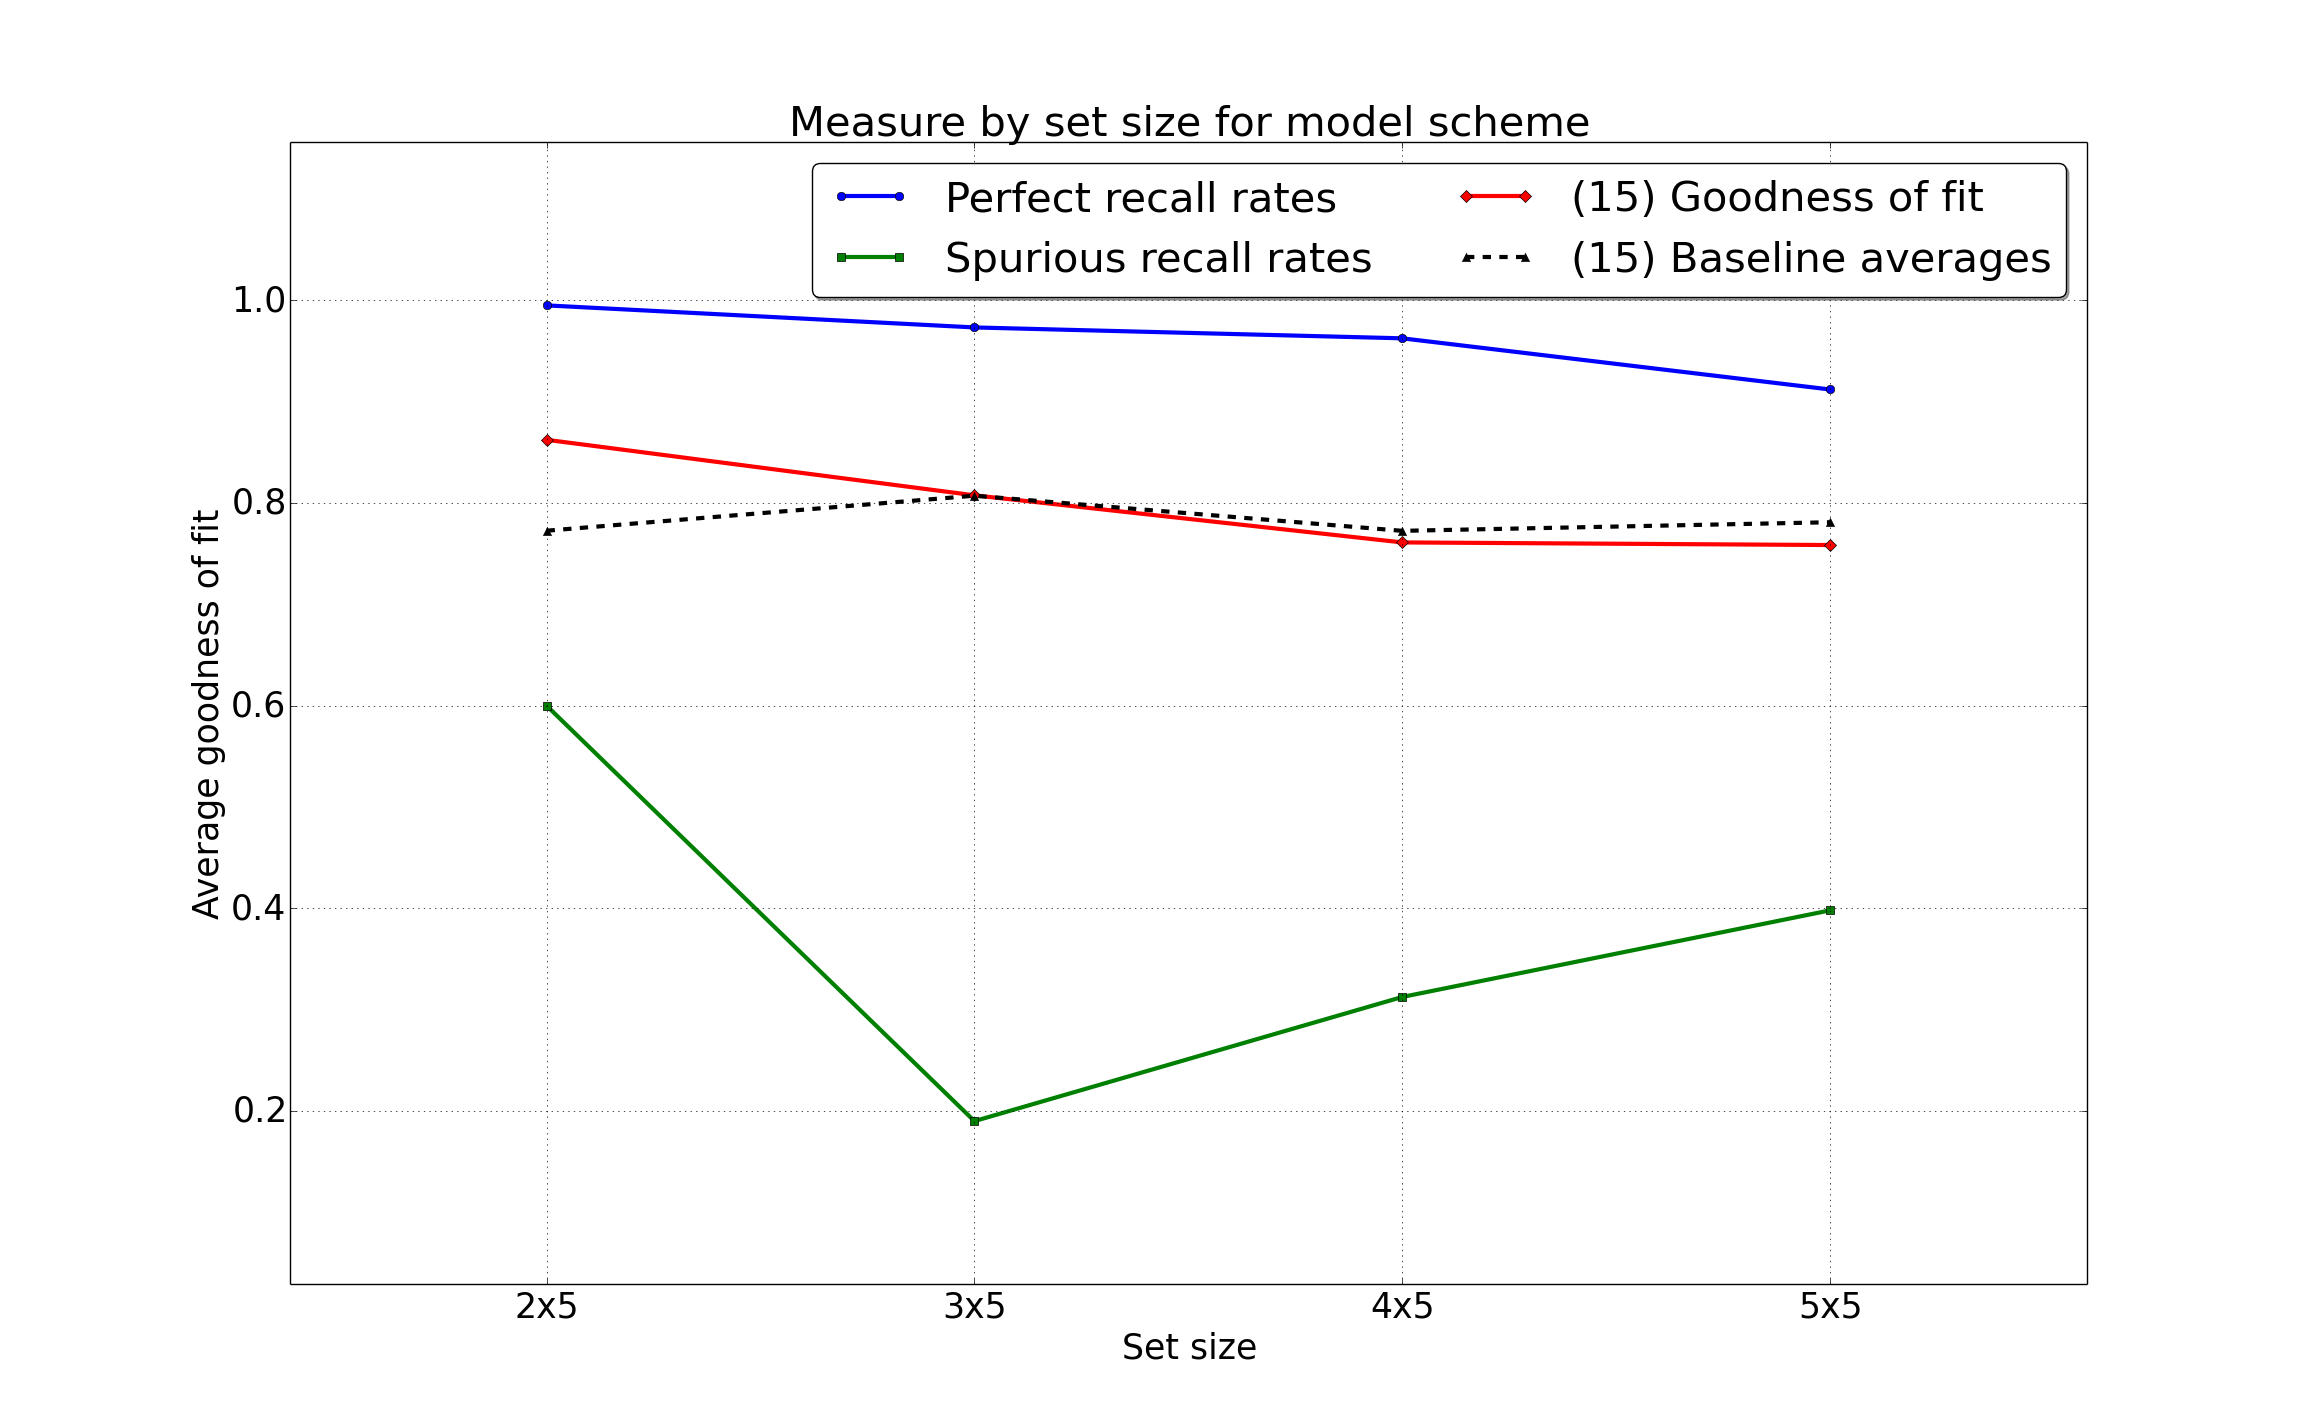
\includegraphics[width=13cm]{fig/hypothesis-test-sync/combined-measures-sync-tr50-tm1-dgw25}
    \caption{Displaying the \textbf{goodness of fit, perfect recall, and spurious recall rates} for the dual-network memory model when using synchronous CA3-layer updating, $\tau=0.50$, DGW$=25$, turnover for every training iteration, and the extracted output by chaotic recall as the training set (both input and outout) for the neocortical network.}
    \label{fig:combined-measures-sync-tr50-tm1-dgw25}
\end{figure}

\begin{figure}
    \centering
    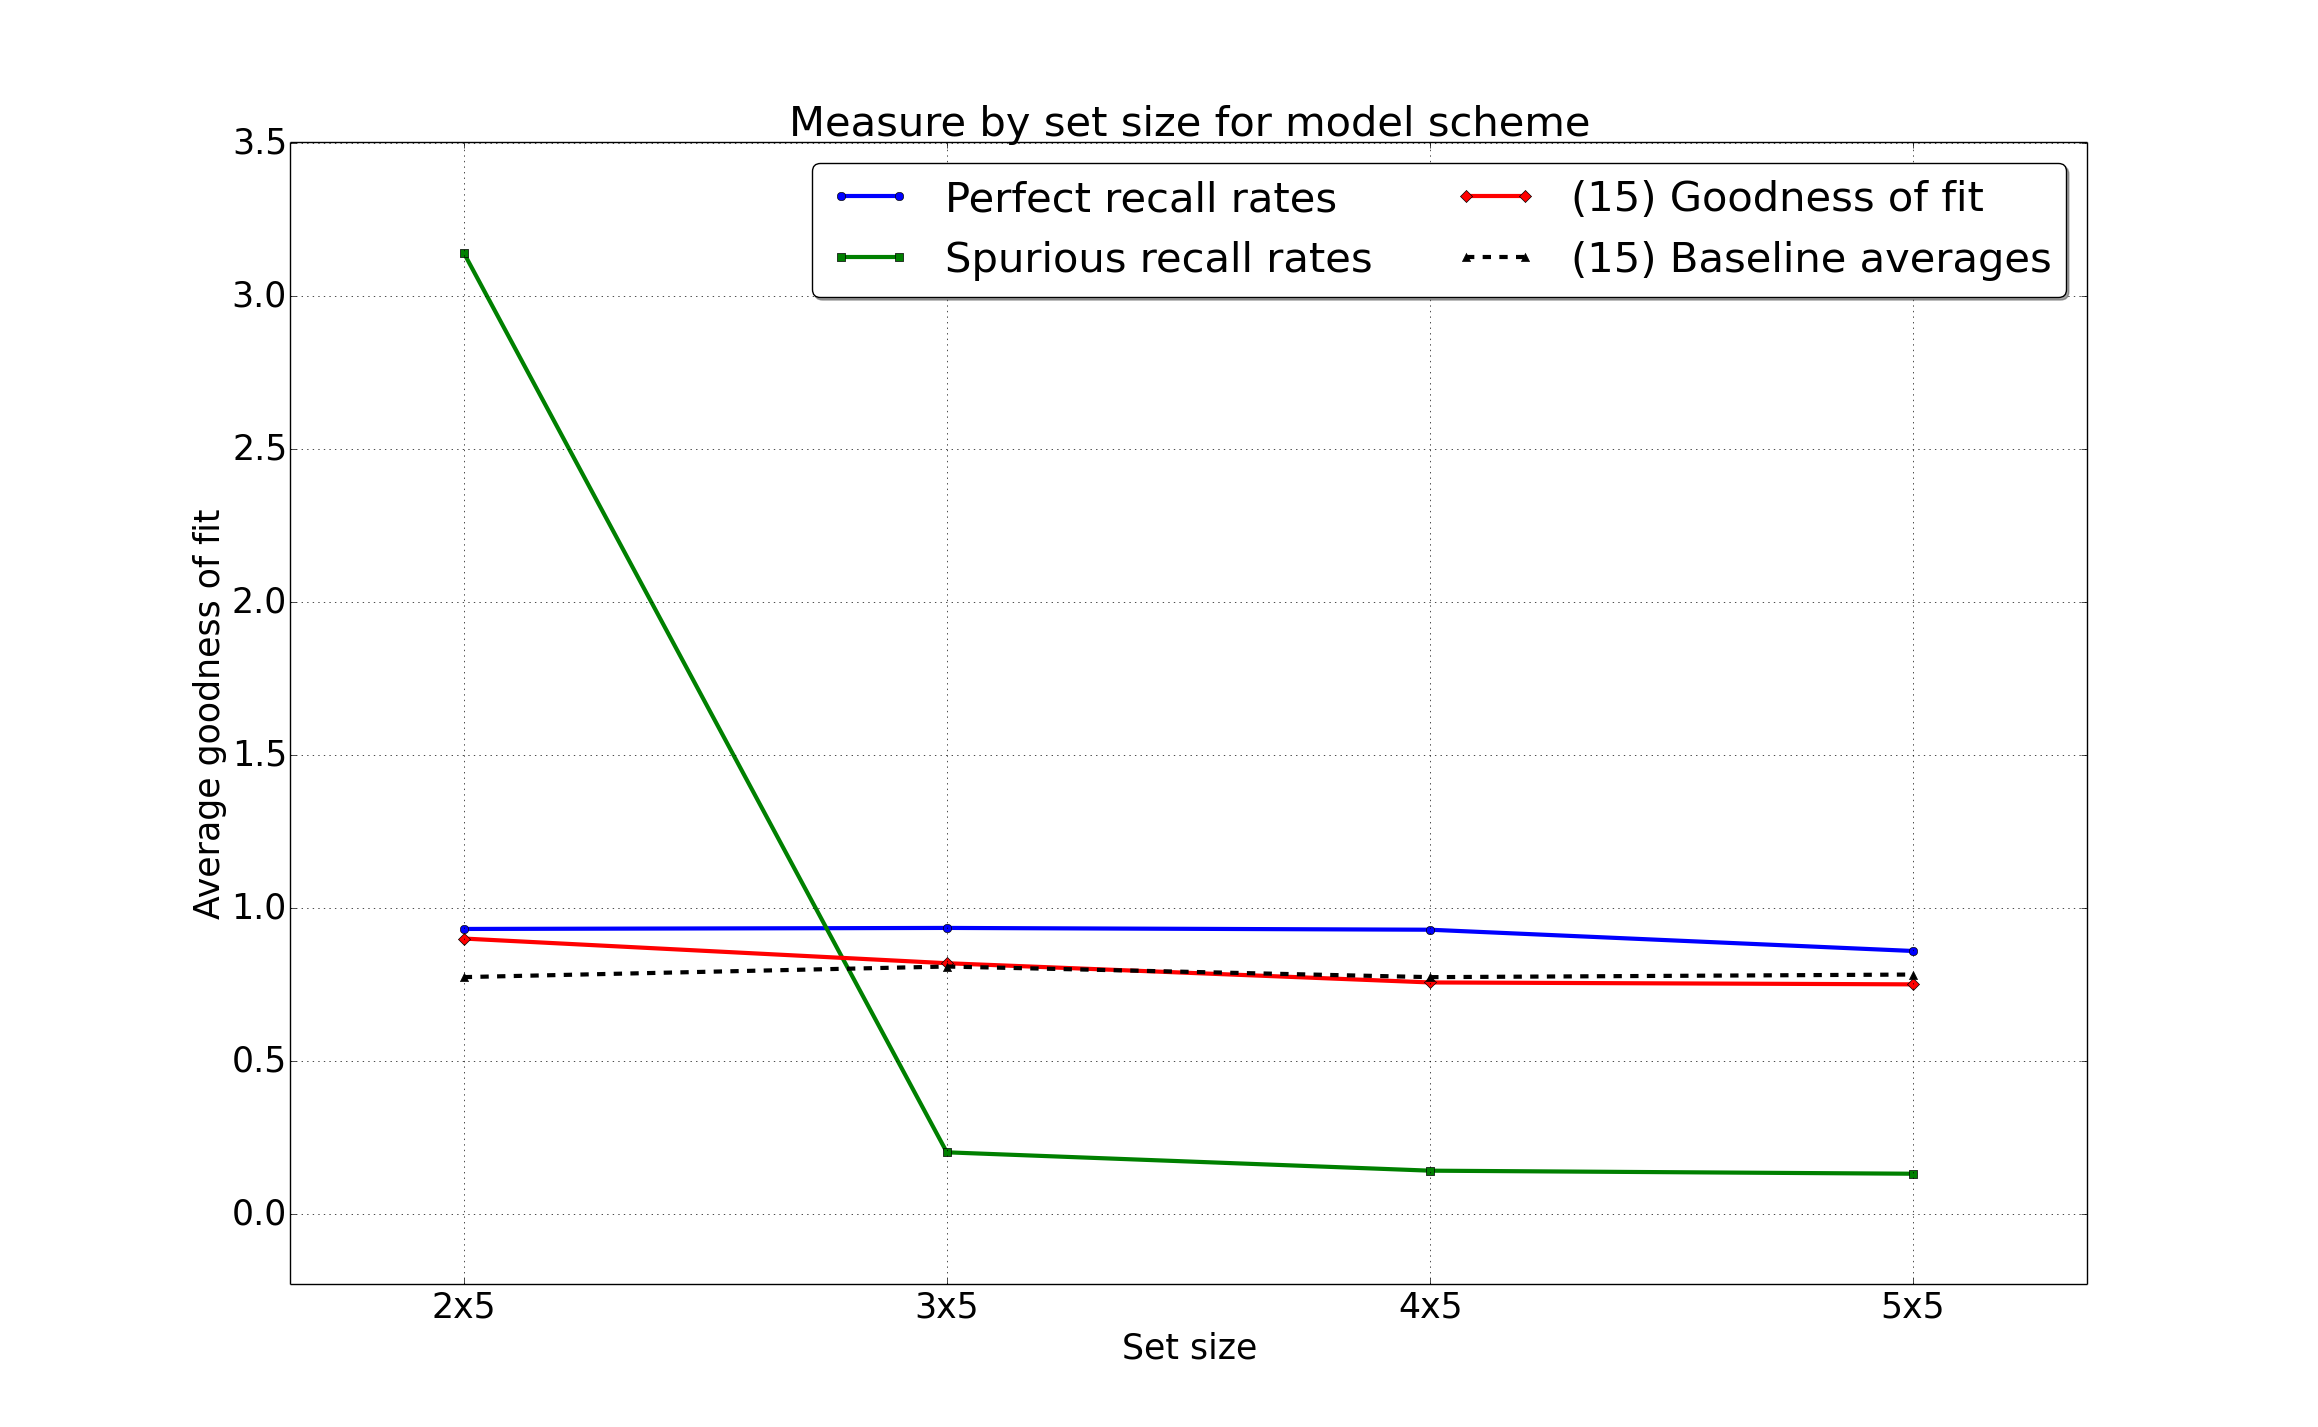
\includegraphics[width=13cm]{fig/hypothesis-test-sync/combined-measures-sync-tm1-tr30-relative-iters}
    \caption{A figure of the \textbf{main measures} as plotted in figure \ref{fig:combined-measures-sync-tr50-tm1-dgw25}, only that the number of \textbf{training iterations in the hippocampal module were set relative to the total set size}, by a factor of $1.5$.}
    \label{fig:combined-measures-sync-tm1-tr30-relative-iters}
\end{figure}

These results indicate that the hypothesis formed above about the number of spurious patterns being crucial to the successful reduction in catastrophic forgetting does not hold. However, the hippocampal model still separates patterns in weight space, resulting in less disruption of old patterns when learning new - i.e. successful reduction of catastrophic forgetting.

\subsection{Comparative results}


\begin{table}[]
\centering
\caption{Showing the average goodness of fit for the best hippocampal model scheme, using only the chaotically recalled pattern outputs for memory consolidation in the novel scheme, along with the approximate goodness of fit from both \citep{Hattori2014}, and \citep{Hattori2010}, both employing pseudorehearsal.}
\label{table:comparison-goodness-of-fit}
\begin{tabular}{c|c|c|c|c|}
\cline{2-5}
                                                      & \multicolumn{4}{c|}{Perfect recall rates} \\ \hline
\multicolumn{1}{|c|}{Pattern set size}                & 2x5      & 3x5      & 4x5      & 5x5      \\ \hline
\multicolumn{1}{|c|}{Conventional model, \citep{Hattori2010}}              & 0.82     & 0.79     & 0.69     & 0.68     \\ \hline
\multicolumn{1}{|c|}{Conventional model, \citep{Hattori2014}}              & 0.97     & 0.95     & 0.91     & 0.89     \\ \hline
\multicolumn{1}{|c|}{Novel model, no pseudorehearsal} & 0.92     & 0.83     & 0.79     & 0.78     \\ \hline
\end{tabular}
\end{table}

Notice that despite using no pseudorehearsal, model performance is significantly better than the model of \citep{Hattori2010}, which is likely due to its lower hippocampal extraction rate. Anyhow, it is noteworthy that the goodness of fit is only slightly lower than the conventional goodnesses of fit when using pseudorehearsal. In fact, when globalising the training set constructed by all chaotically extracted pattern outputs, i.e. training over all extracted outputs, an average goodness of fit of $\approx 0.97-1.00$, is attained. This suggests that the hippocampal patterns contain some qualities which adds a significant robustness to the learning process during memory consolidation using gradient descent in the neocortical network (or FFBP ANN). It was empirically observed that when creating multiple copies of the original training patterns, evenly copying them, and permuting them only a little, the resulting goodness of fit drops fairly quickly as the training set size increases, and furthermore also as the number of training iterations increases. Training iteration sensitivity was displayed when creating only two copies of each training pattern, for which $10 \%$ of the patterns are permuted and distorted. Note that this is in contrast to when training on the chaotically extracted patterns. Possible explanations for this observed emergent model behaviour under the chaotic output as IO scheme includes those outlined above for extracting and encoding the principal components, as well as encoding the pattern recoding and separation in weight space into all pattern outputs. This may then be what is reflected in the successful significant reduction in catastrophic forgetting, and equal to or significantly better than baseline model performance. Note also that an increased sensitivity to the number of training patterns when copying and permuting the original training patterns is expected, because increasing the number of training iterations will 'overfit' the network fairly quickly to the actual permutation, as the model will regard these as undistorted, target patterns. Thus overfitting occurs relative to the original, actual undistorted training patterns. In other words, using only few training iterations $i$, such as to $i=15$, will tend to neglect some of the erroneous details of the permuted training patterns, possibly (and empirically on average) resulting in a better goodness of fit than when increasing the number of iterations to a number such as $i=200$. Nevertheless, it is noteworthy that a greater number of patterns, acquired only from subsets, and trained on only as subsets, successfully leads the neocortical network to attain a fairly good goodness of fit, readable output letters, and a significant robustness to the number of training iterations.


% ========================== Subsection =========================
\subsection{Neocortical module results summary}

A summary of the neocortical module experiments is presented within the list below:

\begin{itemize}
    \item Solely using chaotically recalled patterns with the random input consolidates little or no information.
    \item Using the chaotically recalled patterns (output) as IO to the neocortical network reduces catastrophic interference. This is likely due to the fact that the inclusion of spurious patterns in the extracted patterns by chaotic recall introduces reduction in overlap in the weight space for the consecutive training patterns and subsets, as neuronal turnover and pattern recoding constantly occurs. This is confirmed by the results from the global training schemes, as the performance remains approximately similar.
    \item Using the chaotic output as IO in the global scheme globalizes the training set. This enables the FFBP ANN to extract the principal components, i.e. minimize the error-loss function in the weight-space spanning across all of the chaotic pattern outputs. This results in a performance (goodness of fit) near the case of simply iterating over the entire original training set, but results in worse performance than when using the chaotically extracted output from the local hippocampal training schemes.
    \item Using the chaotically extracted outputs from the most successfull hippocampal model scheme as IO-patterns to the neocortical network introduces a robustness to the learning procedure. This robustness is regarded as the insensitivity to the number of training iterations used, the fairly rapid convergence, as well as by allowing the long-term memory to learn only local subsets of the entire training set sequentially, yet disrupting former subsets fairly little. This is in contrast to when using the chaotically extracted patterns when using asynchronous CA3-updating in the hippocampal module, when training on the subsets of the original training set, or when training on the entire training set when only slightly permuting copies of the original patterns are regarded as the new training set.
\end{itemize}

Shortly put, the mechanism of using the chaotically extracted output patterns as both input and output to the neocortical network ameliorates catastrophic interference, but only in the local training scheme. Using this novel memory consolidation scheme also introduces interesting and desired qualities to the dual-network memory model, such as eliminating the need to pseudorehearsal, which may be regarded as more biologically realistic, and by introducing a robustness to the learning process in terms of training iterations.


% ========================== notes ============================
% \section*{Result notes}

% [This has been factored into the neo. section. However, may include in future work.]
% Although possibly unrealistic, spanning outputs for chaotically recalled patterns and creating a global training set results in a goodness of fit near 1, which is nearly the same performance as for the clean, undistorted, globalised training set - i.e. the best possible performance.
% When training on the subsets sequentially, the performance drops to the 0.7-0.8 interval. HOWEVER, when training on the subsets constructed by spanning over the chaotically recalled OUTPUT, performance rises significantly; > 0.8.
% This may suggest that information separating the patterns in weight space is contained within the spuriously generated patterns. Furthermore, when inspecting the experiments in which the best consolidation quality was achieved using local training of the neocortical module, large numbers of spurious patterns were present. In fact, the empirical data, as well as figure [not yet created], strongly suggests that the spurious patterns are crucial to consolidating the patterns to the neocortical network. Furthermore, they seem to be enabling interleaving of old memories with new implicitly. I hypothesise that this is either by stimulating the long-term memory network in such a way that the weight configuration is less disrupted, or because the strongest pattern-correlation information is contained within these spurious patterns, thus increasing the goodness of fit measure. Addressing the first hypothesis: It may be suggested that this is a viable and fairly biologically realistic mechanism for interleaving patterns, which of course will be in synthesis with further mechanisms, by considering that the output may in fact be relayed back by the CA1-layer, and thus the EC and CA1 activity may be relayed to a long-term memory network, where the chaotically recalled pattern may span a network, stimulating it for consolidation. By considering that FFBP ANNs may be regarded to in fact attain fairly biologically realistic properties on the network level, in contrast to prior historical belief within the field, this view is not implausible.
% Addressing the latter, less complex hypothesis; it is likely that the spurious patterns reflect to some extent the current and former network configuration, as the activity after a constant, continuous flow of recall has occurred. Therefore, I regard the latter as the most likely explanation. Note, however, that this does not disregard the possible implications for how biological consolidation mechanisms might work.


% ========= for all ==========

% appears to be a significant correlation between the convergence rate and the perfect recall rate. this probably correlates with most positive emergent attributes that we wish to attain in the HPC network


% ========================== section ============================
% Experiment design
% Results
% Comparisons

% Enforce sparsity through weight updates corresponding only to the winners of kWTA - didn't work.

% New random pattern each time stability was reached may enhance recall. In either case: unrealistic.

% Convergence when turnover is removed between set iterations?

% It would be interesting to see HPC expanded to include neo. nets activity fed back into the hpc net. in order to induce activity. Perhaps this may cycle through previous patterns. Expanding the model towards Wakagi (08), and using a kind of reverberation could be a focal point in future work.

% Possibly subsets of neurons doing updates synchronously, so subset asynchronicity. Might be that async. is unsuccessful in convergence due to separation.


\cleardoublepage
